\documentclass[12pt,spanish,Letterpaper,openany]{book}
\usepackage{lmodern}
\usepackage{setspace}
\setstretch{1.0}
\usepackage{amssymb,amsmath}
\usepackage{ifxetex,ifluatex}
\usepackage{fixltx2e} % provides \textsubscript
\ifnum 0\ifxetex 1\fi\ifluatex 1\fi=0 % if pdftex
  \usepackage[T1]{fontenc}
  \usepackage[utf8]{inputenc}
\else % if luatex or xelatex
  \ifxetex
    \usepackage{mathspec}
  \else
    \usepackage{fontspec}
  \fi
  \defaultfontfeatures{Ligatures=TeX,Scale=MatchLowercase}
    \setmainfont[Scale=0.92, HyphenChar=None]{Open Sans}
    \setsansfont[]{Open Sans}
    \setmonofont[Mapping=tex-ansi]{Open Sans}
\fi
% use upquote if available, for straight quotes in verbatim environments
\IfFileExists{upquote.sty}{\usepackage{upquote}}{}
% use microtype if available
\IfFileExists{microtype.sty}{%
\usepackage{microtype}
\UseMicrotypeSet[protrusion]{basicmath} % disable protrusion for tt fonts
}{}
\usepackage[left=8.5mm,right=8.5mm,top=11mm,bottom=20mm]{geometry}
\usepackage{hyperref}
\hypersetup{unicode=true,
            pdftitle={Decimo Septima Edicion - Agrotecnología},
            pdfauthor={Escuela de Ingeniería en Ciencias y Sistemas - ECYS},
            pdfborder={0 0 0},
            breaklinks=true}
\urlstyle{same}  % don't use monospace font for urls
\ifnum 0\ifxetex 1\fi\ifluatex 1\fi=0 % if pdftex
  \usepackage[shorthands=off,main=spanish]{babel}
\else
  \usepackage{polyglossia}
  \setmainlanguage[]{spanish}
\fi
\usepackage{natbib}
\bibliographystyle{apalike}
\usepackage{longtable,booktabs}
\usepackage{graphicx,grffile}
\makeatletter
\def\maxwidth{\ifdim\Gin@nat@width>\linewidth\linewidth\else\Gin@nat@width\fi}
\def\maxheight{\ifdim\Gin@nat@height>\textheight\textheight\else\Gin@nat@height\fi}
\makeatother
% Scale images if necessary, so that they will not overflow the page
% margins by default, and it is still possible to overwrite the defaults
% using explicit options in \includegraphics[width, height, ...]{}
\setkeys{Gin}{width=\maxwidth,height=\maxheight,keepaspectratio}
\IfFileExists{parskip.sty}{%
\usepackage{parskip}
}{% else
\setlength{\parindent}{0pt}
\setlength{\parskip}{6pt plus 2pt minus 1pt}
}
\setlength{\emergencystretch}{3em}  % prevent overfull lines
\providecommand{\tightlist}{%
  \setlength{\itemsep}{0pt}\setlength{\parskip}{0pt}}
\setcounter{secnumdepth}{5}

%%% Use protect on footnotes to avoid problems with footnotes in titles
\let\rmarkdownfootnote\footnote%
\def\footnote{\protect\rmarkdownfootnote}


  \title{Decimo Septima Edicion - Agrotecnología}
    \author{Escuela de Ingeniería en Ciencias y Sistemas - ECYS}
      \date{2020-08-21}

%%%%%%%%%%%%%%%%%%%%%%%%%%%%%%%%%%%%%%%%%%%%%%%INIT PREAMBLE%%%%%%%%%%%%%%%%%%%%%%%%%%%%%%%%%%%%%%%%%%%%%%%


%% Opcion que renueva los comandos para el cambio de seccion, el comando por defecto para cada cambio de
%%% seccion genera una pagina en limpio, por lo tanto se renueva el comando definiendo que no se
%%% realice ese cambio, dado que no es funcionan para la edicion de la revista.
%%% Se define para la seccion frontmatter (portada, editorial y contenido) la numeracion de la pagina 
%%% en formato arabico, para la mainmatter (seccion principal - capitulos) la numeracion en numeracion romana (numeros
%%% enteros), y para seccion backmatter ningun tipo de numeracion.
\makeatletter
\renewcommand\mainmatter{\clearpage\@mainmattertrue\pagenumbering{arabic}}
\renewcommand\frontmatter{\clearpage\@mainmatterfalse\pagenumbering{roman}}
\renewcommand\backmatter{\clearpage\@mainmatterfalse}
\makeatother



%% Paquete para el manejo de titulos de capitulos y secciones
\usepackage[explicit,pagestyles]{titlesec}
%% Paquete para uso de urls
\usepackage{url}
%% Paquete utilizado para establecer doble columna en la redaccion de articulos
\usepackage{multicol}
%% Paquete para parametro H, ejemplo: \begin{Figure}[H]
\usepackage{float}
%% Paquete para Enmarcado de Biografia Estudiante, ejemplo: \begin{tcolorbox}...
\usepackage{tcolorbox}
%% Paquete para cargar portada y contraportada, ejemplo: 
\includepdf{01-componentsPDF/cover.pdf}
%% Manual: http://mirrors.ucr.ac.cr/CTAN/macros/latex/contrib/pdfpages/pdfpages.pdf
\usepackage{pdfpages}
%% Paquete para cargar paginas de disenio, ejemplo: \AddEverypageHook{%
\usepackage[contents={},opacity=1,scale=1.5,color=blue!90]{background}
%% Paquete para usar instruccion \ifthenelse
\usepackage{ifthen}
%% Paquete para la definicion de footers y headers
\usepackage{fancyhdr}
%% Paquete complemento para definir tamanio de texto al setear footer y headers
\usepackage{varwidth}
%% Paquete para uso de region sombreada utilizada en titulos de la revista
\usepackage{framed}
%% Paquete utilizado para redefinir tabulacion de vinietas
\usepackage{enumitem}
%% Paquete para colocar imagen en una posicion en especifico
\usepackage[absolute,overlay]{textpos}
\setlength{\TPHorizModule}{1mm}
\setlength{\TPVertModule}{1mm}
%% Paquete utilizado para manejo de colores para links
\usepackage{xcolor}


%% Opcion que define el cambio de linea colocando '-', a las urls demasiado grandes
\def\UrlBreaks{\do\/\do-}

%% Definicion de Comando que acepta un valor numerico y agrega un cero a la izquierda
%%% en el caso que el numero sea menor a 10, se ocupa para la numeracion de las 
%%% paginas iniciales
\newcommand\twodigits[1]{%
   \ifnum#1<10 0#1\else #1\fi
}

%% Instruccion que define a las imagenes la posibilidad de tener un link (interno o
%%% externo activo; se utiliza para enlazar las imagenes a los capitulos definidos
%%% en la hoja del contenido
\ifxetex
  \usepackage{letltxmacro}
  \setlength{\XeTeXLinkMargin}{1pt}
  \LetLtxMacro\SavedIncludeGraphics\includegraphics
  \def\includegraphics#1#{% #1 catches optional stuff (star/opt. arg.)
    \IncludeGraphicsAux{#1}%
  }%
  \newcommand*{\IncludeGraphicsAux}[2]{%
    \XeTeXLinkBox{%
      \SavedIncludeGraphics#1{#2}%
    }%
  }%
\fi

%%%%%%%%%%%%%%%%%%%%%%%INIT Definicion de Numeracion de Paginas%%%%%%%%%%%%%%%%%%%%

%% Seteo de Numero de Pagina, con 2 digitos (01-99) y numeros en negritas %
\newcommand{\etiquetaNumberPage}{%
  %% Manual comando \fontspec: http://mirrors.ucr.ac.cr/CTAN/macros/latex/contrib/fontspec/fontspec.pdf %
  %% \fontspec{(font name)}[(font features)] %
  %%% Es uno de los comandos ad hoc más adecuados para probar y cargar fuentes de forma única. %
  \fontspec{%
    %% Nombre de Fuente Instalada en la carpeta Fonts de Windows "C:\Windows\Fonts" %
    MyriadPro-Bold%
  }[%
    %% SizeFeatures={Size=(X)} %%
    %%% opcion que define diferentes caracteristias para diferentes tamanios de fuente; %
    %%% se utiliza un tamanio (x=numero) con la caracteristica "Size". %
    %
    %% Tamanio de Fuente: 17 %
            SizeFeatures={Size=28},%
    %% Color=(color) %
    %%% Utiliza especificaciones del font para establecer el color del texto.
    %
    %% Color del Texto: Blanco
            Color=white,%
    %% WordSpace={x} %
    %%% toma un factor de escala para escalar el valor predeterminado de espacio entre palabras
    %
    %% Valor para espacio entre palabras: 0 - estrecho %
            %WordSpace=0.0,%
    %% LetterSpace={x}%
    %%% termino dado a sumar (o restar) una pequenia cantidad de espacio horizontal entre caracteres %
    %%% adyacentes; toma un argumento numérico; es un factor aditivo normalizado (no un factor de % 
    %%% escala); Se define como un porcentaje del tamaño de fuente. %
    %
    %% valor de espaciado entre letras: -11.8 - muy estrecho%
            %LetterSpace=-2.5%
  ]%
  %% Commando \twodigits{numero} %
  %%%  devuelve numero en formato de 2 digitos (01-99) %
  \twodigits{%
    %% comando \thepage %
    %%% indica el numero de pagina %
    \thepage%
  }%
}
%%%%%%%%%%%%%%%%%%%%%%%END Definicion de Numeracion de Paginas%%%%%%%%%%%%%%%%%%%%%%%

%%%%%%%%%%%%%%%%%%%%%%%INIT Definicion de Etiquetas de Revista%%%%%%%%%%%%%%%%%%%%%%%

%% Seteo Etiqueta Ciencias, Sistemas y Tecnologia, vinculada con el enlace
%% de la Escuela de Ingenieria en Ciencias y Sistemas
\newcommand{\etiquetaCienciasSistemasTecnologia}{%
  %% Manual comando \fontspec: http://mirrors.ucr.ac.cr/CTAN/macros/latex/contrib/fontspec/fontspec.pdf %
  %% \fontspec{(font name)}[(font features)] %
  %%% Es uno de los comandos ad hoc más adecuados para probar y cargar fuentes de forma única. %
  \fontspec{%
    %% Nombre de Fuente Instalada en la carpeta Fonts de Windows "C:\Windows\Fonts" %
    ArbutusSlab-Regular%
  }[%
    %% SizeFeatures={Size=(X)} %%
    %%% opcion que define diferentes caracteristias para diferentes tamanios de fuente; %
    %%% se utiliza un tamanio (x=numero) con la caracteristica "Size". %
    %
    %% Tamanio de Fuente: 12 %
            SizeFeatures={Size=9.5},%
    %% Color=(color) %
    %%% Utiliza especificaciones del font para establecer el color del texto.
    %
    %% Color del Texto: Blanco
            Color=white,%
    %% WordSpace={x} %
    %%% toma un factor de escala para escalar el valor predeterminado de espacio entre palabras
    %
    %% Valor para espacio entre palabras: 0 - estrecho %
            %WordSpace=0.8,%
    %% LetterSpace={x}%
    %%% termino dado a sumar (o restar) una pequenia cantidad de espacio horizontal entre caracteres %
    %%% adyacentes; toma un argumento numérico; es un factor aditivo normalizado (no un factor de % 
    %%% escala); Se define como un porcentaje del tamaño de fuente. %
    %
    %% valor de espaciado entre letras: -4.5 - estrecho%
            %LetterSpace=-4.5%
  ]%
  %% \href{(url)}{(description)} %
  \href{https://dtt-ecys.org/magazine/public_edicionRevista}{CIENCIAS, SISTEMAS} 
  \vspace{-1.5mm}
  
  
  \href{https://dtt-ecys.org/magazine/public_edicionRevista}{\& TECNOLOGÍA} 
}

%% Seteo Etiqueta Facultad de Ingenieria, vinculada con el enlace
%% de la pagina de ingenieria
\newcommand{\etiquetaFacultadDeIngenieria}{%
  %% Manual comando \fontspec: http://mirrors.ucr.ac.cr/CTAN/macros/latex/contrib/fontspec/fontspec.pdf %
  %% \fontspec{(font name)}[(font features)] %
  %%% Es uno de los comandos ad hoc más adecuados para probar y cargar fuentes de forma única. %
  \fontspec{%
    %% Nombre de Fuente Instalada en la carpeta Fonts de Windows "C:\Windows\Fonts" %
    ArbutusSlab-Regular%
  }[%
    %% SizeFeatures={Size=(X)} %%
    %%% opcion que define diferentes caracteristias para diferentes tamanios de fuente; %
    %%% se utiliza un tamanio (x=numero) con la caracteristica "Size". %
    %
    %% Tamanio de Fuente: 17 %
            SizeFeatures={Size=9.5},%
    %% Color=(color) %
    %%% Utiliza especificaciones del font para establecer el color del texto.
    %
    %% Color del Texto: Blanco
            Color=white,%
    %% WordSpace={x} %
    %%% toma un factor de escala para escalar el valor predeterminado de espacio entre palabras
    %
    %% Valor para espacio entre palabras: 0 - estrecho %
            %WordSpace=0.0,%
    %% LetterSpace={x}%
    %%% termino dado a sumar (o restar) una pequenia cantidad de espacio horizontal entre caracteres %
    %%% adyacentes; toma un argumento numérico; es un factor aditivo normalizado (no un factor de % 
    %%% escala); Se define como un porcentaje del tamaño de fuente. %
    %
    %% valor de espaciado entre letras: -11.8 - muy estrecho%
            %LetterSpace=-4.5%
  ]%
  %% \href{(url)}{(description)} %
  \href{https://portal.ingenieria.usac.edu.gt/}{FACULTAD DE} 
  \vspace{-1mm}
  
  
  \href{https://portal.ingenieria.usac.edu.gt/}{INGENIERÍA} 
}
%%%%%%%%%%%%%%%%%%%%%%%END Definicion de Etiquetas de Revista%%%%%%%%%%%%%%%%%%%%%%%

%%%%%%%%%%%%%%%%%INIT Aplicando Estilos de Numeros de Pagina y Etiquetas de Revista%%%%%%%%%%%%%%%%%


%% Seteo de Numero de Pagina en la parte derecha, para paginas pares (Even)
\newcommand{\nodeNumberPageEast}{%
  %% Manual comando \node: http://mirrors.ucr.ac.cr/CTAN/graphics/pgf/base/doc/pgfmanual.pdf %
  \node[%
    %% /tikz/anchor=(anchor) %
    %%% Specifies an anchor of the node; %
    %
    %% anclaje abajo izquierda %
        anchor=south west,% 
    %% /tikz/text=(color) %
    %%% Sets the color to be used for text labels; %
    %
    %% color de texto blanco %
        text=white,%
    %% /tikz/execute at begin node=(code) %
    %%% Esta opcion hace que (code) se ejecute al principio de un nodo
        execute at begin node={\begin{varwidth}{\textheight}}, %
    %% /tikz/execute at end node=(code) %
    %%% Esta opcion instala (code) que se ejecutará al final del nodo
        execute at end node={\end{varwidth}}%
  ]%
  %
  %% Current Page Node – Absolute Positioning %
  %% There is a special node called current page that can be used to access the current page. %
  %
  %% ubicacion de pagina abajo derecha %
  at ([xshift=-16.5mm,yshift=2mm] current page.south east)% 
  {\etiquetaNumberPage};%
}

%% Seteo de Numero de Pagina en la parte izquierda, para paginas impares (Odd)
\newcommand{\nodeNumberPageWest}{%
  %% Manual comando \node: http://mirrors.ucr.ac.cr/CTAN/graphics/pgf/base/doc/pgfmanual.pdf %
  \node[%
    %% /tikz/anchor=(anchor) %
    %%% Specifies an anchor of the node; %
    %
    %% anclaje abajo izquierda %
        anchor=south west,% 
    %% /tikz/text=(color) %
    %%% Sets the color to be used for text labels; %
    %
    %% color de texto blanco %
        text=white,%
    %% /tikz/execute at begin node=(code) %
    %%% Esta opcion hace que (code) se ejecute al principio de un nodo
        execute at begin node={\begin{varwidth}{\textheight}}, %
    %% /tikz/execute at end node=(code) %
    %%% Esta opcion instala (code) que se ejecutará al final del nodo
        execute at end node={\end{varwidth}}%
  ]%
  %
  %% Current Page Node – Absolute Positioning %
  %% There is a special node called current page that can be used to access the current page. %
  %
  %% ubicacion de pagina abajo izquierda %
  at ([xshift=1.5mm,yshift=2mm] current page.south west)%
  {\etiquetaNumberPage};%
}

%% Comando que establece la posicion horizontal de la Etiqueta Ciencias, Sistemas y Tecnologia %
%% Por medio del comando \node%
\newcommand{\nodeHorizontalPositionCienciasSistemasTecnologia}{%
  %% Manual comando \node: http://mirrors.ucr.ac.cr/CTAN/graphics/pgf/base/doc/pgfmanual.pdf %
  \node[%
    %% /tikz/text=(color) %
    %%% Sets the color to be used for text labels; %
    %
    %% color de texto blanco %
    text=white, %
    %% /tikz/execute at begin node=(code) %
    %%% Esta opcion hace que (code) se ejecute al principio de un nodo
    execute at begin node={\begin{varwidth}{\textheight}}, %
    %% /tikz/execute at end node=(code) %
    %%% Esta opcion instala (code) que se ejecutará al final del nodo
    execute at end node={\end{varwidth}}%
  ]%
  %
  %% Current Page Node – Absolute Positioning %
  %% There is a special node called current page that can be used to access the current page. %
  %
  %% ubicacion de pagina abajo derecha %
  at ([xshift=-92.50mm,yshift=7.7mm]current page.south east)%
  {\etiquetaCienciasSistemasTecnologia};%
}
%% Comando que establece la posicion horizontal de la Etiqueta Facultad de Ingenieria %
%% Por medio del comando \node%
\newcommand{\nodeHorizontalPositionFacultadDeIngenieria}{%
  %% Manual comando \node: http://mirrors.ucr.ac.cr/CTAN/graphics/pgf/base/doc/pgfmanual.pdf %
  \node[%
    %% /tikz/text=(color) %
    %%% Sets the color to be used for text labels; %
    %
    %% color de texto blanco %
    text=white, %
    %% /tikz/execute at begin node=(code) %
    %%% Esta opcion hace que (code) se ejecute al principio de un nodo
    execute at begin node={\begin{varwidth}{\textheight}}, %
    %% /tikz/execute at end node=(code) %
    %%% Esta opcion instala (code) que se ejecutará al final del nodo
    execute at end node={\end{varwidth}}%
  ]%
  %
  %% Current Page Node – Absolute Positioning %
  %% There is a special node called current page that can be used to access the current page. %
  %
  %% ubicacion de pagina abajo izquierda %
  at ([xshift=90.0mm,yshift=8.0mm]current page.south west)
  {\etiquetaFacultadDeIngenieria};%
}

%% Aplicando segundo estilo de numeracion y etiquetas
%%% Numeracion parte inferior derecha e izquierda 
%%%% numeros impares = izquierda: Footer Odd
%%%% numeros pares = derecha: Footer Even
%%%
%%% Etiquetas parte derecha e izquierda
%%%% etiqueta Facultad de Ing. = izquierda: Footer Odd
%%%% etiqueta Ciencias Sistemas. = Derecha: Footer Even
%%%
%% Comando con nombre "fancyplainstyle", que identifica el
%%% primer estilo a representar en la revista.
\newcommand{\fancyplainstyleTwo}{
  %% Comando que limpia cualquier personalizacion antes realizada
  %%% para el borrado completo no agregar ningun parametro "{}"
  \fancyhf{}
  %% Definiendo etiqueta horizontal Ciencias Sistemas
  %% Definiendo numero de pagina par
  %%% \fancyfoot[places]{field}
  \fancyfoot[E]{
    %% Comando que se define para establecer posicion absoluta de
    %%% etiqueda de acuerdo a las posiciones defindas en la declaracion
    %%% del comando \nodeHorizontalPosition...
    \begin{tikzpicture}[overlay, remember picture]%
      \nodeNumberPageEast
      \nodeHorizontalPositionCienciasSistemasTecnologia
    \end{tikzpicture}
  }
  %% Definiendo etiqueta horizontal Facultad de Ing.
  %% Definiendo numero de pagina impar
  %%% \fancyfoot[places]{field}
  \fancyfoot[O]{
    %% Comando que se define para establecer posicion absoluta de
    %%% etiqueda de acuerdo a las posiciones defindas en la declaracion
    %%% del comando \nodeHorizontalPosition...
    \begin{tikzpicture}[overlay, remember picture]%
      \nodeNumberPageWest
      \nodeHorizontalPositionFacultadDeIngenieria
    \end{tikzpicture}
  }
}

%% Declarando comando que establece el primer tipo de estilo a todas las paginas,
%%% asi como tambien a las paginas donde se define el titulo del articulo,
%%% dado que el disenio es diferente al resto de las paginas.
\newcommand{\setPageStyleTwo}{%
  %% Definiendo el estilo a todas las paginas
  \pagestyle{fancy}{\fancyplainstyleTwo}
  %% Definiendo el mismo estilo a paginas que tiene el encabezado de titulo
  \fancypagestyle{plain}{\fancyplainstyleTwo}
}

%% Borrando estilos de paginas que forman parte del frontmatter (editorial y
%%% contenido), dado que dichas paginas tienen una estructura unica
\fancypagestyle{plain}{%
  %% Comando que limpia cualquier personalizacion antes realizada
  %%% para el borrado completo no agregar ningun parametro "{}"
  \fancyhf{}%
}

%% Estableciendo tamanio de encabezado debido a warning mostrado al generar
%%% documento PDF, se establecio la longiutd de 15pt, por solicitud en contenido
%%% del mensaje mostrado en dicho warning.
\setlength{\headheight}{15pt}

%% El segmento de encabezado y pie de pagina, por default cuentan con una linea
%%% que divide los segmentos con el contenido del documento, por disenio de revista
%%% las lineas no son requeridas, por lo tanto se define el grosor de la linea con
%%% valor 0 (cero).
\renewcommand{\headrulewidth}{0pt}
\renewcommand{\footrulewidth}{0pt}

%%%%%%%%%%%%%%%%%%END Aplicando Estilos de Numeros de Pagina y Etiquetas de Revista%%%%%%%%%%%%%%%%%

%%%%%%%%%%%%%%INIT Definicion Region sombreada para titulo y datos de author de articulo   2C6093  426190   %%%%%%%%%%%%%%
\definecolor{titlePart1Contenido}{HTML}{284A5E}
\definecolor{titlePart2Contenido}{HTML}{3D5C6E}
\definecolor{fondo}{HTML}{FFFFFF}
\definecolor{fondotitulo}{HTML}{FFFFFF}
\definecolor{imagetitle}{HTML}{222930}
\definecolor{autorinfoData}{HTML}{222930}
\definecolor{styleAuthorNameColor}{HTML}{5A7199}
\colorlet{shadecolor}{fondotitulo}
%%%%%%%%%%%%%%END Definicion Region sombreada para titulo y datos de author de articulo%%%%%%%%%%%%%%

%%%%%%%%%%%%%%INIT Dehabilitando Titulo y Autor por Default%%%%%%%%%%%%%%
\AtBeginDocument{\let\maketitle\relax}
%%%%%%%%%%%%%%END Dehabilitando Titulo y Autor por Default%%%%%%%%%%%%%%

%%%%%%%%%%%%%%INIT Propiedades de Parrafos, tabulaciones, vinietas, etc.%%%%%%%%%%%%%%

%% Cambiando longitud (setlength) de sangria de parrafos (\parindent)
%%% 1em es equivalente al espacio de una 'M' de acuerdo al tipo y tamanio de fuente.
\setlength{\parindent}{1em}
%% Cambiando longitud (setlist) de venietas (itemsize)
%%% 1em es equivalente al espacio de una 'M' de acuerdo al tipo y tamanio de fuente.
\setlist[itemize]{labelindent = \parindent, leftmargin=*}

%% Redefiniendo longitud minima de fraccion de texto ocupado en una pagina de texto
%%% valor por defecto 0.2
\renewcommand{\textfraction}{0.05}
%% Redefiniendo longitud maxima de fraccion de una pagina de texto ocupada por objetos
%%% flotantes en la parte superior, valor por defecto 0.7
\renewcommand{\topfraction}{0.8}
%% Redefiniendo longitud maxima de fraccion de una pagina de texto ocupada por objetos
%%% flotantes en la parte inferior, valor por defecto 0.3
\renewcommand{\bottomfraction}{0.8}
%% Redefiniendo longitud minima de fraccion de una pagina de texto ocupada por objetos
%%% flotantes que puede ser usada por los mismo, valor por defecto 0.5
\renewcommand{\floatpagefraction}{0.75}

%% Comando que establece el uso de espacio normal despues del signo '.'
\frenchspacing
%% La configuracion influye en la rutina de salto de parrafo en si misma: los cambios en 
%% \tolerance en realidad afectan a que saltos de linea se eligen. Los valores mas altos 
%% permiten que se acepten lineas peores (lo que generalmente significa: con espacios entre 
%% palabras estirados), con el valor que 10000indica un "modo de panico" donde cualquier cosa 
%% es aceptable. Normalmente, cuanto mas bajo sea el valor, mejor se vera el parrafo, pero corre 
%% el riesgo de reducir tanto la lista de posibles saltos que terminara con lineas demasiado llenas.
\tolerance=5000
%% quita la restriccion para igualar el contenido de la pagina (justificacion vertical)
\raggedbottom
%%%%%%%%%%%%%%END Propiedades de Parrafos, tabulaciones, vinietas, etc.%%%%%%%%%%%%%%

%%%%%%%%%%%%%%INIT Propiedades MultiColumnas%%%%%%%%%%%%%%
%% que contiene el valor de \pretolerance dentro de un entorno multicols 
\multicoltolerance=3000 
%% quita la restriccion para igualar el contenido en columnas (justificacion vertical)
\raggedcolumns
%% Espacio entre columnas esta controlado por el parámetro \setlength{\columnsep}
\setlength{\columnsep}{2em}
%We want a rule between columns.
%\setlength\columnseprule{.4pt}

%Tambien queremos asegurarnos de que un nuevo entorno multicols 
%encuentre suficiente espacio en la parte inferior de la página.
\setlength\premulticols{6\baselineskip}

%Al equilibrar columnas, ignoramos las soluciones que son 
%demasiado malas. Además, si la última columna es demasiado mala, 
%la tipeamos sin estirar.
\setcounter{columnbadness}{7000}
\setcounter{finalcolumnbadness}{7000}
%%%%%%%%%%%%%%END Propiedades MultiColumnas%%%%%%%%%%%%%%

\newenvironment{photobiography3}[1]%
{%
\begin{textblock}{20}(11.25,11.90)%
      \includegraphics[width=32.809mm, height=32.809mm]{#1}%
\end{textblock}%
\begin{minipage}{195.0mm}\begin{flushright}\small%
\color{white}\fontsize{10.0}{10}\fontspec{MyriadPro-Regular}%\addfontfeatures{LetterSpace=-1.00}%%\color{autorinfoData}\fontsize{11}{11}\fontspec{MyriadPro-Regular}%\addfontfeatures{LetterSpace=-1.00}%
}%
{%
	\end{flushright}\end{minipage}%
	%\hspace{0.5mm}%
}

\newenvironment{photobiography4}%
{%
\begin{tcolorbox}[colback=fondo, colframe=fondo, width=92.19mm, boxsep=-2mm, arc=0mm]
\begin{minipage}{90.19mm}%
	\hspace{1mm}%
	\hspace{2.19mm}%
	\begin{minipage}{89.00mm}\begin{flushleft}\small%
	\vspace{3mm}%
}%
{%
  \vspace{3mm}%
	\end{flushleft}\end{minipage}%
	%\hspace{0.5mm}%
\end{minipage}%
\end{tcolorbox}
}


\newenvironment{styleAuthorName}
  {\color{styleAuthorNameColor}\fontsize{14}{14}\fontspec{MyriadPro-Regular}\addfontfeatures{LetterSpace=1.85}\selectfont}% \begin{styleAuthorName}
  {}% \end{styleAuthorName}
  
\newenvironment{styleAuthormail}
  {\vspace{-0.1mm}\color{white}\fontsize{10.2}{10}\fontspec{MyriadPro-Bold}\selectfont}%
  {\vspace{2.30mm}}%
  
  \newenvironment{styleKeywords}
  {\vspace{1.75mm}\fontsize{9.5}{10}\selectfont}%
  {}%
  
  \newenvironment{styleKeywordsTwo}
  {\vspace{1.75mm}\fontsize{9.5}{10}\selectfont}%
  {\vspace{2.4mm}}%
  

\newenvironment{boldenv}
  {\bfseries}% \begin{boldenv}
  {}% \end{boldenv}
  
\newenvironment{normalsizeenv}
  {\normalsize}% \begin{normalsizeenv}
  {}% \end{normalsizeenv}
  
\newenvironment{smalltextenv}
  {\begin{center}\kern-1em\color{imagetitle}\small}% \begin{smalltextenv}
  {\end{center}}% \end{smalltextenv}
  
\newenvironment{centerimageenv}
  {\noindent \begin{center}}% \begin{centerimageenv}
  {\end{center}}% \end{centerimageenv}
  
\newenvironment{hypertargetimageenv}[1]
{\hypertarget{#1}{}% \begin{hypertargetimageenv}
{}}% \end{hypertargetimageenv}

\newcommand{\spacetext}{\vspace{8.1mm}}
\newcommand{\minimalspacetext}{\vspace{1mm}}
\newcommand{\spaceelevenmilis}{\vspace{11mm}}
\newcommand{\spacetenmilis}{\vspace{10mm}}
\newcommand{\spaceninemilis}{\vspace{9mm}}
\newcommand{\spaceeightmilis}{\vspace{8mm}}
\newcommand{\spacesevenmilis}{\vspace{7mm}}
\newcommand{\spacesixmilis}{\vspace{6mm}}
\newcommand{\spacefivemilis}{\vspace{5mm}}
\newcommand{\spacefourmilis}{\vspace{4mm}}
\newcommand{\spacethreemilis}{\vspace{3mm}}
\newcommand{\spacetwomilis}{\vspace{2mm}}
\newcommand{\spaceonemilis}{\vspace{1mm}}
\newcommand{\spaceminusmilis}{\vspace{-0.5mm}}
\newcommand{\spaceinitialeditorialcontenido}{\vspace{-10.1mm}}

%%%%%%%%%%%%%%%%%%%%%%%%%%%%%%%%%%%%%%INIT contenido%%%%%%%%%%%%%%%%%%%%%%%%%%%%%%%%%%%%%%

%%%%%%%%%%%%%%%%%%%%%%%%%%%%%%%%%INIT Imagenes contenido%%%%%%%%%%%%%%%%%%%%%%%%%%%%%%%%%
\newcommand{\imagecontenidoparteone}{%
\begin{textblock}{20}(-3.86,30.12)%
}
\newcommand{\imagecontenidopartetwo}{%
\end{textblock}%
\begin{textblock}{20}(117.80,38.77)%
}
\newcommand{\imagecontenidopartethree}{%
\end{textblock}%
\begin{textblock}{20}(117.80,105.35)%
}
\newcommand{\imagecontenidopartefour}{%
\end{textblock}%
}
%%%%%%%%%%%%%%%%%%%%%%%%%%%%%%%%%%END Imagenes contenido%%%%%%%%%%%%%%%%%%%%%%%%%%%%%%%%%

%%%%%%%%%%%%%%%%%%%%%%%%%%%%%%%%%INIT Linea contenido%%%%%%%%%%%%%%%%%%%%%%%%%%%%%%%%%
\newenvironment{segmentocontenido}
{%
\begin{flushleft}%
  \begin{tcolorbox}[colback=white, colframe=white, width=\textwidth, boxsep=-2mm, arc=0mm]%
    \begin{minipage}{\textwidth}%
}% \begin
{%
    \end{minipage}%
  \end{tcolorbox}%
\end{flushleft}%
}% \end

\newenvironment{panelnumeropaginatitulo}
{%
\begin{minipage}[c]{83.00mm}%
}% \begin
{%
\end{minipage}%
}% \end

\newenvironment{panelnumeropagina}
{%
\begin{minipage}[c]{13.00mm}%
  \fontspec{MyriadPro-Regular}[Color=white]\bfseries%
}% \begin
{%
\end{minipage}%
}% \end

\newenvironment{paneltitulo}
{%
\hspace{3mm}%
\begin{minipage}[c]{68.00mm}%
  \fontspec{ArbutusSlab-Regular}[SizeFeatures={Size=10},Color=white,LetterSpace=-4.5]\bfseries%
}% \begin
{%
  \end{minipage}%
}% \end

\newcommand{\lineacontenidoparteone}{%
\spacetwomilis%
\begin{segmentocontenido}%
  \hspace{7mm}%
  \begin{panelnumeropaginatitulo}%
    \begin{panelnumeropagina}%
}
\newcommand{\lineacontenidopartetwo}{%
    \end{panelnumeropagina}%
    \begin{paneltitulo}%
}
\newcommand{\lineacontenidopartethree}{%
    \end{paneltitulo}%
  \end{panelnumeropaginatitulo}%
  \hspace{8mm}%
  \begin{panelnumeropaginatitulo}%
    \begin{panelnumeropagina}%
}
\newcommand{\lineacontenidopartefour}{%
    \end{panelnumeropagina}%
    \begin{paneltitulo}%
}
\newcommand{\lineacontenidopartefive}{%
    \end{paneltitulo}%
  \end{panelnumeropaginatitulo}%
\end{segmentocontenido}%
}
%%%%%%%%%%%%%%%%%%%%%%%%%%%%%%%%%%END Linea contenido%%%%%%%%%%%%%%%%%%%%%%%%%%%%%%%%%
%%%%%%%%%%%%%%%%%%%%%%%%%%%%%%%%%%%%%%END contenido%%%%%%%%%%%%%%%%%%%%%%%%%%%%%%%%%%%%%%

%%%%%%%%%%%%%%%%%%%%%%%%%INIT Formato de Titulo%%%%%%%%%%%%%%%%%%%%%%%%%
\newcommand{\formatchapter}{\normalfont\color{black}\begin {shaded*}\bfseries}
\newcommand{\labelchapter}{\empty}
\newcommand{\sepchapter}{-25pt}
\newcommand{\beforecodechapter}{\filcenter\LARGE}
\newcommand{\beforecodechapterparttwo}{\end{shaded*}}

\newcommand{\formatchapterEdDQ}{\begin {flushright}}
\newcommand{\labelchapterEdDQ}{\empty}
\newcommand{\sepchapterEdDQ}{165pt}
\newcommand{\beforecodechapterEdDQ}{\color{white}\fontsize{18}{19}\fontspec{Arial-BoldMT}\addfontfeatures{LetterSpace=1.85}\selectfont}
\newcommand{\beforecodechapterparttwoEdDQ}{\end{flushright}}

\newcommand{\leftchapterEdDQ}{0pt}

\newcommand{\beforesepchapterEdDQ}{-28.1pt}
\newcommand{\beforesepchapterEdDQDobleLine}{-33.35pt}

\newcommand{\afterchapterEdDQ}{-25.00pt}
\newcommand{\afterchapterEdDQDobleLine}{-35.00pt}

\newcommand{\noformatchapter}{\normalfont\bfseries}
\newcommand{\nolabelchapter}{\labelchapter}
\newcommand{\nosepchapter}{0pt}
\newcommand{\nobeforecodechapter}{\Huge}

\newcommand{\leftchapter}{0pt}
\newcommand{\beforesepchapter}{-22pt}
\newcommand{\afterchapter}{-25pt}

\newcommand{\formatsection}{\fontspec{Open Sans Condensed}[SizeFeatures={Size=16},Color=black,LetterSpace=-1.5]}
\newcommand{\labelsection}{\empty}
\newcommand{\sepsection}{0.0em}
\newcommand{\beforecodesection}{\bfseries\selectfont}

\newcommand{\formatsubsection}{\fontspec{Open Sans Condensed}[SizeFeatures={Size=15},Color=black!80,LetterSpace=-1.5]}
\newcommand{\labelsubsection}{\empty}
\newcommand{\sepsubsection}{0.0em}
\newcommand{\beforecodesubsection}{\bfseries\selectfont}


\newcommand{\formatsubsubsection}{\fontspec{Open Sans Condensed}[SizeFeatures={Size=13},Color=black!60,LetterSpace=-1.5]}
\newcommand{\labelsubsubsection}{\empty}
\newcommand{\sepsubsubsection}{0.0em}
\newcommand{\beforecodesubsubsection}{\bfseries\selectfont}


%%%%%%%%%%%%%%%%%%%%%%%%%%END Formato de Titulo%%%%%%%%%%%%%%%%%%%%%%%%%

%%%%%%%%%%%%%%%%%%%%%%%%%%%%%%%%%%%%%%%%%%%%%%%END PREAMBLE%%%%%%%%%%%%%%%%%%%%%%%%%%%%%%%%%%%%%%%%%%%%%%%
\newcommand{\hideFromPandoc}[1]{#1}
\hideFromPandoc{ \let\Begin\begin \let\End\end }
\newcommand{\minipagepartone}{\begin{minipage}[c]{7.5cm}}
\newcommand{\minipagetwocolumn}{\noindent\begin{minipage}[c]{\columnwidth}}
\newcommand{\minipageparttwo}{\end{minipage}\begin{minipage}[c]{12.0cm}\begin{flushleft}\begin{normalsizeenv}\begin{boldenv}}
\newcommand{\minipageendpart}{\end{boldenv}\end{normalsizeenv}\end{flushleft}\end{minipage}}
\newcommand{\floatbeginfigure}{\begin{figure}[H] \centering}
\newcommand{\floatendfigure}{\end{figure}}
\newcommand{\changeStyleNameInit}{\begin{styleAuthorName}}
\newcommand{\changeStyleNameEnd}{\end{styleAuthorName}}
\newcommand{\changeStyleMailInit}{\begin{styleAuthormail}}
\newcommand{\changeStyleMailEnd}{\end{styleAuthormail}}
\newcommand{\changeStyleKeyWordsInit}{\begin{styleKeywords}}
\newcommand{\changeStyleKeyWordsEnd}{\end{styleKeywords}}
\newcommand{\changeStyleKeyWordsTwoInit}{\begin{styleKeywordsTwo}}
\newcommand{\changeStyleKeyWordsTwoEnd}{\end{styleKeywordsTwo}}

\let\BeginKnitrBlock\begin \let\EndKnitrBlock\end
\begin{document}
\maketitle

%%%%%%%%%%%%%%%%%%%%%%%%%%%%%%%%%%%%%%%%%%%%%%%INIT FRONTCOVER%%%%%%%%%%%%%%%%%%%%%%%%%%%%%%%%%%%%%%%%%%%%%%%

%% Archivo que agrega la portada (cover) a revista al iniciar el contenido y
%%% define el disenio de la revista

%% Manual: http://mirrors.ucr.ac.cr/CTAN/macros/latex/contrib/pdfpages/pdfpages.pdf
%
%% \includepdf[(key=val)]{(filename)}
%%% Inserta páginas de un documento PDF externo.
%
%% Comando que agrega la contraportada (archivo con extension .pdf) al iniciar
%%% el contenido de la revista
%%%%%%%%%%%%%%%%%%%%%%%%%%%%%%%%%%%%%%
\includepdf{01-componentsPDF/cover.pdf}


\includepdf[picturecommand*={%
    %X,%Y%
    \put(118.0,325.0){\textcolor{white}{\fontspec{Arial Black}[SizeFeatures={Size=40}]{\protect\hyperlink{article07}{AGROTECNOLOGÍA}}}}%'AGROTECNOLOGÍA','AGROTECNOLOGÍA ',' UNA OPCIÓN PARA LA AGRICULTURA GUATEMALTECA'
    \put(118.0,305.00){\textcolor{white}{\fontspec{Arial}[SizeFeatures={Size=16}]{\protect\hyperlink{article07}{UNA OPCIÓN PARA LA AGRICULTURA GUATEMALTECA}}}}%
    \put(255,219){\textcolor{white}{\fontspec{Arial Black}[SizeFeatures={Size=18}]{\protect\hyperlink{article01}{BLOCKCHAIN}}}}%'BLOCKCHAIN','EN GUATEMALA'
    \put(255,203){\textcolor{white}{\fontspec{Arial}[SizeFeatures={Size=14}]{\protect\hyperlink{article01}{EN GUATEMALA}}}}%
    \put(255,173){\textcolor{white}{\fontspec{Arial Black}[SizeFeatures={Size=18}]{\protect\hyperlink{article12}{RECONOCIMIENTO DE PATRONES}}}}%'RECONOCIMIENTO DE PATRONES','E INTELIGENCIA ARTIFICIAL'
    \put(255,153){\textcolor{white}{\fontspec{Arial}[SizeFeatures={Size=14}]{\protect\hyperlink{article12}{E INTELIGENCIA ARTIFICIAL}}}}%
    \put(255,113){\textcolor{white}{\fontspec{Arial Black}[SizeFeatures={Size=18}]{\protect\hyperlink{article14}{MULTI-CLOUD}}}}%'MULTI-CLOUD','UNA ESTRATÉGIA PARA LA REDUCCIÓN DE COSTOS'
    \put(255,98){\textcolor{white}{\fontspec{Arial}[SizeFeatures={Size=14}]{\protect\hyperlink{article14}{UNA ESTRATÉGIA PARA LA REDUCCIÓN DE COSTOS}}}}%
    \put(255,69){\textcolor{white}{\fontspec{Arial Black}[SizeFeatures={Size=18}]{\protect\hyperlink{article09}{ADICCIONES TECNOLÓGICAS}}}}%'ADICCIONES TECNOLÓGICAS'
    \put(25.0,20){\href{https://qrco.de/bbIeeT}{\includegraphics[width=1.042in,height=1.042in]{01-componentsPDF/coverQR.png}}}%
}]{01-componentsPDF/cover.pdf}

%

%% Comando que define la estructura general para establecer el disenio de pagina 
%% Acepta como parametro, el path relativo de la imagen [1].
\newcommand{\setBackgroundImage}[1]{%
  %% Comando que establece los valores para establecer el fondo (background)
  \backgroundsetup{%
    %% scale=(x) donde x: cualquier valor positivo %
    %%% cambia el factor de escala que se aplicará al material de fondo %
    %
    % Seteo de scala = 1, normal %
    scale=1,%
    %% opacity=(x) donde x: cualquier valor entre 0 y 1 %
    %%% cambia el nivel de transparencia para el material de fondo %
    %%% valores: de 0 (transparencia total) hasta 1 (sin transparencia) %
    %
    % Seteo de opacidad = 1, sin transparencia (fondo original)
    opacity=1,%
    %% angle=(x) donde x: cualquier valor entre -360 y 360%
    %%% especifica el angulo para el material de fondo que se utilizará en el documento. %
    %%% Los angulos se miden en sentido antihorario %
    %
    % Seteo de angulo: 0, fondo en posicion original (angulo 0) %
    angle=0,%
    %% contents=(content) donde content: Text, images, etc%
    %%% opción le permite al usuario especificar el material que se utilizará %
    %%% en el documento. Este material puede ser bastante arbitrario: texto de %
    %%% longitud arbitraria, imágenes incluidas mediante el comando estándar %
    %%% \includegraphics del paquete graphicx, o gráficos creados con el paquete %
    %%% PGF/TikZ, por ejemplo. %
    %
    %% Imagen de fondo que abarca todo el ancho y todo el largo de la pagina %
    contents={%
      %% \includegraphics[(key val list)]{(file)} %
      %%% Comando que agrega (incluye) graficos de acuerdo a un archivo de entrada %
      %
      %% se utiliza el parametro definido en el comando %
      %%% \newcommand{\setBackgroundImage}[1] (#1) para establecer el nombre del %
      %%% archivo a incluir. %
      \includegraphics[%
        %% opcion que define el ancho que tendra la imagen, utilizando el comando %
        %%% \paperwidth, se establece que se ocupara todo el tamanio de dicha pagina %
        width=\paperwidth,%
        %% opcion que define el largo que tendra la imagen, utilizando el comando %
        %%% \paperheight, se establece que se ocupara todo el tamanio de dicha pagina %
        height=\paperheight%
      ]{%
        #1%
      }%
    }%
  }%
}

%% Manual: http://mirrors.ucr.ac.cr/CTAN/macros/latex/contrib/background/background.pdf
%% Comando \AddEverypageHook{(background)[...(background)]}
%%% Comando que agrega 1 o varios backgrounds, dependiendo del disenio de la revista
%%% mediante condiciones.
%
%% El disenio de la revista cuenta con lo siguiente:
%%%% - Fondo personalizado para pagina de editorial
%%%% - Fondo personalizado para pagina de contenido
%%%% - Fondo personalizado (pagina impar y par) para articulos redactados por estudiantes
%%%% - Fondo personalizado (pagina impar y par) para articulos redactados por egresados
%%%% - Fondo personalizado (pagina impar y par) para articulos informativos DTT
\AddEverypageHook{%
%
%% Editorial y Contenido, son capitulos que no son numerados en la revista, dado que son %
%%% parte de la estructura del documento: frontmatter (parte frontal de la revista). %
%%% Por lo tanto son capitulos que tienen valor 0 (cero), en su numero de capitulo. %
%
% \ifthenelse{(boolean function)}{(then clause)}{(else clause)} %
%% Instruccion que comprueba los capitulos que forman parte de frontmatter %
%%% Condicion: numero de capitulo < 1, o igual a cero dado que no existen valores negativos %
\ifthenelse{\thechapter<1}%
{}{}%
%{%
%  %% Condicion pagina = 1, entonces colocar disenio de pagina editorial %
  \ifnum \value{page}=1 \setBackgroundImage{01-componentsPDF/imparEditorial.pdf} \fi%
  %% Condicion pagina = 2, entonces colocar disenio de pagina contenido %
  \ifnum \value{page}=2 \setBackgroundImage{01-componentsPDF/parContenido.pdf} \fi%
%}{}% se definen condiciones independientes, por lo tanto la condicion else no tiene implementacion %
%
%
%% Los capitulos informativos (DTT) serian los capitulo 1 al capitulo 12 %
%
% \ifthenelse{(boolean function)}{(then clause)}{(else clause)} %
%% Condicion: numero de capitulo > 0 Y  pagina < 35, que serian capitulos 1 al 12; %
%%% y el numero 31 indica el numero de pagina donde se encuentra la contraportada, %
%%% sin esta condicion la contraporta tendría el disenio en continuidad %
%%% de los capitulos de la revista %
\ifthenelse{\thechapter>0\AND\value{page}<52}%
{%
  %% Condicion que comprueba cuando una pagina es impar (isodd) %
	\ifthenelse{\isodd{\value{page}}}%
		%% Condicion verdadera (esimpar), %
	  %%% entonces colocar disenio de pagina impar  %
		{%
		  \ifthenelse{\value{page}=1\OR\value{page}=3\OR\value{page}=11\OR\value{page}=21\OR\value{page}=1\OR\value{page}=29\OR\value{page}=33\OR\value{page}=41\OR\value{page}=45\OR\value{page}=49\OR\value{page}=3000}%
      {\setBackgroundImage{01-componentsPDF/imparTitulo.pdf}}% if part%
      {%
        \ifthenelse{\value{page}=3000}%
        {\setBackgroundImage{01-componentsPDF/imparTituloNoFoto.pdf}}% if part%
        {\setBackgroundImage{01-componentsPDF/impar.PDF}}% else part%
      }% else part%
		}%
		%% Condicion false (no es impar, por lo tanto es par), %
		%%% entonces colocar disenio de pagina impar  %
		{%
		  \ifthenelse{\value{page}=5\OR\value{page}=6\OR\value{page}=8\OR\value{page}=16\OR\value{page}=5\OR\value{page}=26\OR\value{page}=38\OR\value{page}=5\OR\value{page}=5\OR\value{page}=5\OR\value{page}=500}%
      {\setBackgroundImage{01-componentsPDF/parTitulo.pdf}}% if part%%
      {%
        \ifthenelse{\value{page}=500\OR\value{page}=500}%
        {\setBackgroundImage{01-componentsPDF/parTituloNoFoto.pdf}}% if part%
        {\setBackgroundImage{01-componentsPDF/par.PDF}}% else part%
      }% else part%
		}%
}{}% se definen condiciones independientes, por lo tanto la condicion else no tiene implementacion %
%
%
%% Comando que forma parte del comando \AddEverypageHook{\bg@material}
\BgMaterial}

%%%%%%%%%%%%%%%%%%%%%%%%%%%%%%%%%%%%%%%%%%%%%%%END FRONTCOVER%%%%%%%%%%%%%%%%%%%%%%%%%%%%%%%%%%%%%%%%%%%%%%%

%%%%%%%%%%%ContenidoTOC%%%%%%%%%%%
%%{
%%\setcounter{tocdepth}{0}
%\tableofcontents
%}
%%%%%%%%%%%%ContenidoTOC%%%%%%%%%%%
\frontmatter

\titleformat{\chapter}[display]{\noformatchapter}{\nolabelchapter}{\nosepchapter}{\nobeforecodechapter}

\hypertarget{editorial}{%
\chapter*{Editorial}\label{editorial}}
\addcontentsline{toc}{chapter}{Editorial}

\spaceinitialeditorialcontenido

Sin duda alguna el campo de la informática y la robótica en general se han visto acelerados en su expansión a lo largo de los últimos años, ello se ha visto reflejado en nuevas áreas de exploración e investigación que han surgido, las cuales han encontrado nuevos campos en otras ramas del conocimiento. Sirviendo como valiosas herramientas de apoyo en cada una de estas disciplinas.

Hoy en día el campo de la exploración tecnológica se entrelaza en sus múltiples disciplinas, en el desarrollo de componentes y sensores físicos, elementos de procesamiento y recolección de datos, así como procesos de aprendizaje y predicción en base a estos datos. El abaratamiento de los costos de procesamiento y almacenamiento, tecnologías en la nube han sido factores clave en viabilizar el acceso a nuevas tecnologías a costos mucho más asequibles.

Es así como, el campo de la Agrotecnología se ha visto impactado positivamente de estos beneficios, facilitando la creación de nuevos sistemas de producción, mecanización y automatización de labores, big data y agricultura de precisión, software de gestión de servicios de información para toma de decisiones, etc.

Todos estos beneficios se vuelven de gran importancia, principalmente para países caracterizados como países agrícolas, tal es el caso de Guatemala, lo cual demanda redoblar los esfuerzos en pro de lograr la transferencia tecnológica en éstas áreas, lo cual puede significar grandes y nuevas oportunidades, pero también implican el riesgo de un mayor rezago de no lograr dicho objetivo.

Ello debido a la eficiencia de los mercados que hoy es demanda, respecto a calidad, tiempos, precios y control de la producción. Lo cual hace un nicho interesante a explorar por los profesionales de informática, pues el paso acelerado y los cambios abruptos del comportamiento social de los últimos tiempos, han demostrado que la presencia tecnológica se irradia como una necesidad a todos los campos de desarrollo, siendo un factor indispensable para su sostenibilidad y subsistencia.

\spacetwomilis

\Begin{flushright}

\textbf{MSc. Ing. Carlos Gustavo Alonzo}\\
Director de la Escuela de Ciencias y Sistemas\\
Facultad de Ingeniería\\
Universidad de San Carlos de Guatemala

\End{flushright}

\begin{textblock*}{\textwidth}(114mm,222.0mm)\fontspec{ArialMTStd-Medium}[SizeFeatures={Size=13}]{\color{white}\href{http://c3.usac.edu.gt/revistasistemas/index.php}{• Revista Ciencias, Sistemas y Tecnología}}\end{textblock*}

\begin{textblock*}{\textwidth}(114mm,228.0mm)\fontspec{ArialMTStd-Medium}[SizeFeatures={Size=13}]{\color{white}\href{https://dtt-ecys.org/magazine/public_edicionRevista}{• Escuela de Ingeniería en Ciencias y Sistemas}}\end{textblock*}

\begin{textblock*}{\textwidth}(114mm,234.0mm)\fontspec{ArialMTStd-Medium}[SizeFeatures={Size=13}]{\color{white}\href{https://issuu.com/revistaecys}{• Revista Ciencias, Sistemas y Tecnología - Issuu.com}}\end{textblock*}

\begin{textblock*}{\textwidth}(116mm,247.250mm)\fontspec{ArialMTStd-Medium}[SizeFeatures={Size=13}]{\color{white}\href{mailto://revista.ecys@gmail.com}{revista.ecys@gmail.com}}\end{textblock*}

\hypertarget{contenido}{%
\chapter*{Contenido}\label{contenido}}
\addcontentsline{toc}{chapter}{Contenido}

\imagecontenidoparteone

\protect\hyperlink{article02}{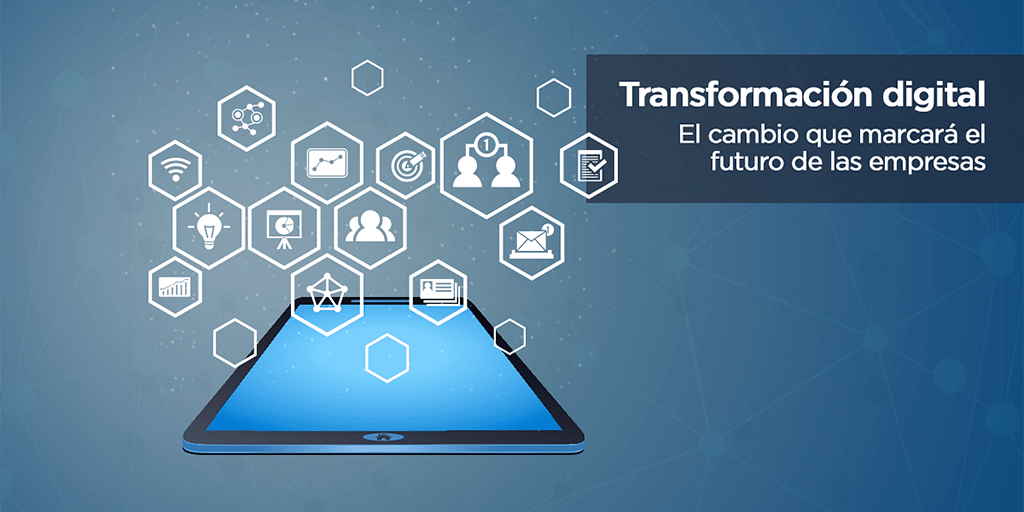
\includegraphics[width=4.8in,height=2.36in]{media/articulo02_image2.png}}

\imagecontenidopartetwo

\protect\hyperlink{article11}{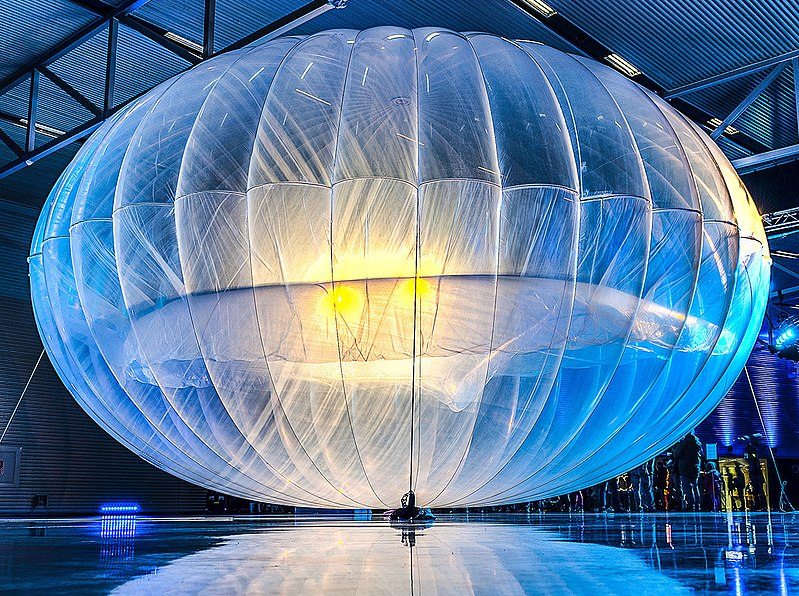
\includegraphics[width=3.7in,height=2.8in]{media/contenido02.jpeg}}

\imagecontenidopartethree

\protect\hyperlink{article06}{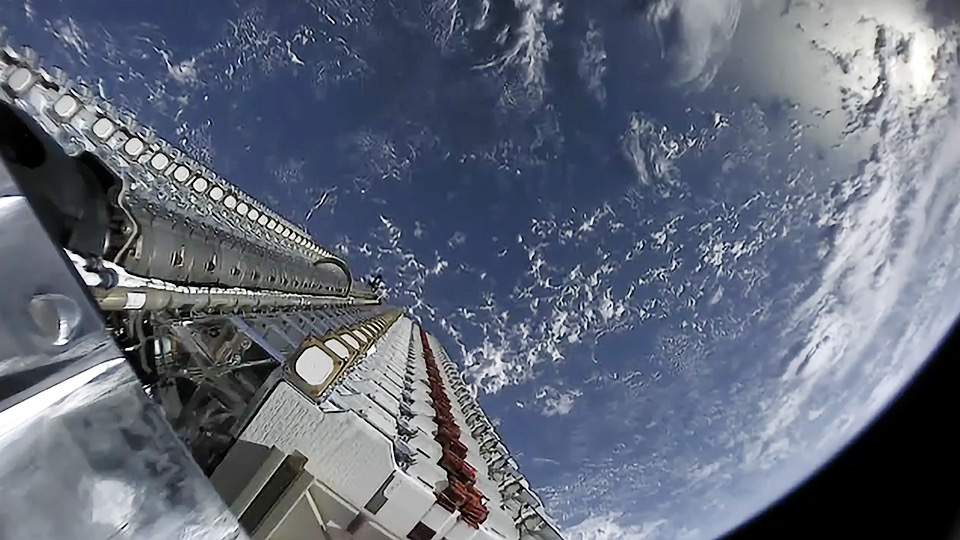
\includegraphics[width=3.711in,height=2.2in]{media/contenido03.jpeg}}

\imagecontenidopartefour

\begin{textblock*}{\textwidth}(24.194mm,93.50mm)\fontspec{Arial Black}[SizeFeatures={Size=10.90}]{\color{titlePart1Contenido}\protect\hyperlink{article01}{Blockchain}}\end{textblock*}

\begin{textblock*}{\textwidth}(-0.78mm,93.4mm)\fontspec{Arial Black}[SizeFeatures={Size=25.90}]{\color{white}\protect\hyperlink{article01}{01}}\end{textblock*}

\begin{textblock*}{\textwidth}(24.2mm,97.5mm)\fontspec{ArialMTStd-Medium}[SizeFeatures={Size=10.45}]{\color{titlePart2Contenido}\protect\hyperlink{article01}{En Guatemala}}\end{textblock*}

\begin{textblock*}{\textwidth}(24.2mm,111.5mm)\fontspec{Arial Black}[SizeFeatures={Size=10.90}]{\color{titlePart1Contenido}\protect\hyperlink{article02}{Qué es la transformación digital}}\end{textblock*}

\begin{textblock*}{\textwidth}(-0.78mm,111.2mm)\fontspec{Arial Black}[SizeFeatures={Size=25.90}]{\color{white}\protect\hyperlink{article02}{03}}\end{textblock*}

\begin{textblock*}{\textwidth}(24.2mm,115.5mm)\fontspec{ArialMTStd-Medium}[SizeFeatures={Size=10.45}]{\color{titlePart2Contenido}\protect\hyperlink{article02}{y cuál es su importancia}}\end{textblock*}

\begin{textblock*}{\textwidth}(24.2mm,128.5mm)\fontspec{Arial Black}[SizeFeatures={Size=10.90}]{\color{titlePart1Contenido}\protect\hyperlink{article03}{Sistemas Operativos}}\end{textblock*}

\begin{textblock*}{\textwidth}(-0.78mm,128.5mm)\fontspec{Arial Black}[SizeFeatures={Size=25.90}]{\color{white}\protect\hyperlink{article03}{06}}\end{textblock*}

\begin{textblock*}{\textwidth}(24.2mm,132.5mm)\fontspec{ArialMTStd-Medium}[SizeFeatures={Size=10.45}]{\color{titlePart2Contenido}\protect\hyperlink{article03}{pasado, actualidad y, ¿olvido?}}\end{textblock*}

\begin{textblock*}{\textwidth}(24.2mm,147.36mm)\fontspec{Arial Black}[SizeFeatures={Size=10.90}]{\color{titlePart1Contenido}\protect\hyperlink{article04}{El Internet para todos}}\end{textblock*}

\begin{textblock*}{\textwidth}(-0.78mm,146.0mm)\fontspec{Arial Black}[SizeFeatures={Size=25.90}]{\color{white}\protect\hyperlink{article04}{08}}\end{textblock*}

\begin{textblock*}{\textwidth}(24.2mm,151.14mm)\fontspec{ArialMTStd-Medium}[SizeFeatures={Size=10.45}]{\color{titlePart2Contenido}\protect\hyperlink{article04}{}}\end{textblock*}

\begin{textblock*}{\textwidth}(24.2mm,163.5mm)\fontspec{Arial Black}[SizeFeatures={Size=10.90}]{\color{titlePart1Contenido}\protect\hyperlink{article05}{IoP y recursos tecnológicos}}\end{textblock*}

\begin{textblock*}{\textwidth}(-0.78mm,163.5mm)\fontspec{Arial Black}[SizeFeatures={Size=25.90}]{\color{white}\protect\hyperlink{article05}{11}}\end{textblock*}

\begin{textblock*}{\textwidth}(24.2mm,167.5mm)\fontspec{ArialMTStd-Medium}[SizeFeatures={Size=10.45}]{\color{titlePart2Contenido}\protect\hyperlink{article05}{para personas con discapacidad}}\end{textblock*}

\begin{textblock*}{\textwidth}(98.25mm,163.1mm)\fontspec{Arial Black}[SizeFeatures={Size=10.90}]{\color{titlePart1Contenido}\protect\hyperlink{article10}{Cloud computing, modelos de capa gratuita}}\end{textblock*}

\begin{textblock*}{\textwidth}(198.99mm,163.1mm)\fontspec{Arial Black}[SizeFeatures={Size=25.90}]{\color{white}\protect\hyperlink{article10}{33}}\end{textblock*}

\begin{textblock*}{\textwidth}(107.40mm,167.1mm)\fontspec{ArialMTStd-Medium}[SizeFeatures={Size=10.45}]{\color{titlePart2Contenido}\protect\hyperlink{article10}{como oportunidad de aprendizaje y capacitación}}\end{textblock*}

\begin{textblock*}{\textwidth}(24.2mm,181.5mm)\fontspec{Arial Black}[SizeFeatures={Size=10.90}]{\color{titlePart1Contenido}\protect\hyperlink{article06}{Nuclear versus}}\end{textblock*}

\begin{textblock*}{\textwidth}(-0.78mm,181.2mm)\fontspec{Arial Black}[SizeFeatures={Size=25.90}]{\color{white}\protect\hyperlink{article06}{16}}\end{textblock*}

\begin{textblock*}{\textwidth}(24.2mm,185.5mm)\fontspec{ArialMTStd-Medium}[SizeFeatures={Size=10.45}]{\color{titlePart2Contenido}\protect\hyperlink{article06}{Renovable}}\end{textblock*}

\begin{textblock*}{\textwidth}(137.80mm,180.96mm)\fontspec{Arial Black}[SizeFeatures={Size=10.90}]{\color{titlePart1Contenido}\protect\hyperlink{article11}{La web descentralizada}}\end{textblock*}

\begin{textblock*}{\textwidth}(198.99mm,180.56mm)\fontspec{Arial Black}[SizeFeatures={Size=25.90}]{\color{white}\protect\hyperlink{article11}{38}}\end{textblock*}

\begin{textblock*}{\textwidth}(155.20mm,185.04mm)\fontspec{ArialMTStd-Medium}[SizeFeatures={Size=10.45}]{\color{titlePart2Contenido}\protect\hyperlink{article11}{un reto en internet}}\end{textblock*}

\begin{textblock*}{\textwidth}(24.2mm,198.86mm)\fontspec{Arial Black}[SizeFeatures={Size=10.90}]{\color{titlePart1Contenido}\protect\hyperlink{article07}{Agrotecnología}}\end{textblock*}

\begin{textblock*}{\textwidth}(-0.78mm,198.26mm)\fontspec{Arial Black}[SizeFeatures={Size=25.90}]{\color{white}\protect\hyperlink{article07}{21}}\end{textblock*}

\begin{textblock*}{\textwidth}(24.2mm,202.86mm)\fontspec{ArialMTStd-Medium}[SizeFeatures={Size=10.45}]{\color{titlePart2Contenido}\protect\hyperlink{article07}{Una opción para la agricultura guatemalteca}}\end{textblock*}

\begin{textblock*}{\textwidth}(128.50mm,198.1mm)\fontspec{Arial Black}[SizeFeatures={Size=10.90}]{\color{titlePart1Contenido}\protect\hyperlink{article12}{Reconocimiento de patrones}}\end{textblock*}

\begin{textblock*}{\textwidth}(198.99mm,198.0mm)\fontspec{Arial Black}[SizeFeatures={Size=25.90}]{\color{white}\protect\hyperlink{article12}{41}}\end{textblock*}

\begin{textblock*}{\textwidth}(150.80mm,202.1mm)\fontspec{ArialMTStd-Medium}[SizeFeatures={Size=10.45}]{\color{titlePart2Contenido}\protect\hyperlink{article12}{e inteligencia artificial}}\end{textblock*}

\begin{textblock*}{\textwidth}(24.2mm,215.96mm)\fontspec{Arial Black}[SizeFeatures={Size=10.90}]{\color{titlePart1Contenido}\protect\hyperlink{article08}{Alta disponibilidad}}\end{textblock*}

\begin{textblock*}{\textwidth}(-0.78mm,215.96mm)\fontspec{Arial Black}[SizeFeatures={Size=25.90}]{\color{white}\protect\hyperlink{article08}{26}}\end{textblock*}

\begin{textblock*}{\textwidth}(24.2mm,219.76mm)\fontspec{ArialMTStd-Medium}[SizeFeatures={Size=10.45}]{\color{titlePart2Contenido}\protect\hyperlink{article08}{con Servicios en la Nube}}\end{textblock*}

\begin{textblock*}{\textwidth}(144.60mm,216.0mm)\fontspec{Arial Black}[SizeFeatures={Size=10.90}]{\color{titlePart1Contenido}\protect\hyperlink{article13}{La batalla de las API}}\end{textblock*}

\begin{textblock*}{\textwidth}(198.99mm,215.6mm)\fontspec{Arial Black}[SizeFeatures={Size=25.90}]{\color{white}\protect\hyperlink{article13}{45}}\end{textblock*}

\begin{textblock*}{\textwidth}(148.30mm,220.0mm)\fontspec{ArialMTStd-Medium}[SizeFeatures={Size=10.45}]{\color{titlePart2Contenido}\protect\hyperlink{article13}{Rest, GraphQL y gRPC}}\end{textblock*}

\begin{textblock*}{\textwidth}(24.2mm,235.11mm)\fontspec{Arial Black}[SizeFeatures={Size=10.90}]{\color{titlePart1Contenido}\protect\hyperlink{article09}{Adicciones Tecnológicas}}\end{textblock*}

\begin{textblock*}{\textwidth}(-0.78mm,233.11mm)\fontspec{Arial Black}[SizeFeatures={Size=25.90}]{\color{white}\protect\hyperlink{article09}{29}}\end{textblock*}

\begin{textblock*}{\textwidth}(24.2mm,237.60mm)\fontspec{ArialMTStd-Medium}[SizeFeatures={Size=10.45}]{\color{titlePart2Contenido}\protect\hyperlink{article09}{}}\end{textblock*}

\begin{textblock*}{\textwidth}(163.00mm,232.91mm)\fontspec{Arial Black}[SizeFeatures={Size=10.90}]{\color{titlePart1Contenido}\protect\hyperlink{article14}{Multi-Cloud}}\end{textblock*}

\begin{textblock*}{\textwidth}(198.99mm,232.91mm)\fontspec{Arial Black}[SizeFeatures={Size=25.90}]{\color{white}\protect\hyperlink{article14}{49}}\end{textblock*}

\begin{textblock*}{\textwidth}(118.00mm,236.91mm)\fontspec{ArialMTStd-Medium}[SizeFeatures={Size=10.45}]{\color{titlePart2Contenido}\protect\hyperlink{article14}{una estrategia para la reducción de costos}}\end{textblock*}

\mainmatter
\setPageStyleTwo

\titleformat{\chapter}[block]{\formatchapterEdDQ}{\labelchapterEdDQ}{\sepchapterEdDQ}{\beforecodechapterEdDQ#1\beforecodechapterparttwoEdDQ}

\titlespacing*{\chapter} {\leftchapterEdDQ}{\beforesepchapterEdDQ}{\afterchapterEdDQ}

\titleformat{\section}[block]{\formatsection}{\labelsection}{\sepsection}{\beforecodesection#1}

\titleformat{\subsection}[block]{\formatsubsection}{\labelsubsection}{\sepsubsection}{\beforecodesubsection#1}

\titleformat{\subsubsection}[block]{\formatsubsubsection}{\labelsubsubsection}{\sepsubsubsection}{\beforecodesubsubsection#1}

\hypertarget{article01}{%
\chapter{Blockchain en Guatemala}\label{article01}}

\BeginKnitrBlock{photobiography3}{media/articulo01_image1.png}
\begin{styleAuthorName}

Kevin Alberto Morán Orellana

\end{styleAuthorName}
\begin{styleAuthormail}

\textbf{\href{mailto:kevinalbertoorellana@gmail.com}{\nolinkurl{kevinalbertoorellana@gmail.com}}}

\end{styleAuthormail}

Estudiante de Ingeniería en Ciencias y Sistemas - USAC

\begin{styleKeywordsTwo}

\textbf{Palabras Clave:}\\
Blockchain, Guatemala.

\end{styleKeywordsTwo}
\EndKnitrBlock{photobiography3}

\Begin{multicols}{2}

Blockchain fue desarrollada y propuesta hace casi 30 años pero no fue utilizado sino hasta el 2009 cuando Satoshi Nakamoto, pseudónimo detrás del cual no se sabe quién está, lo usó como base para el hoy tan famoso ``Bitcoin''. Principalmente ha sido asociado a las criptomonedas, por ser la base de estas, pero sus aplicaciones abarcan mucho más allá de eso, por ejemplo: registros de historial médico, registro de votos en elecciones, trazabilidad de productos, etc.

Traducido Blockchain significa ``cadena de bloques''. Esto debido a que cuando se quiere ingresar un nuevo registro es generado un bloque de información el cual al ser verificado es ingresado a la cadena de manera secuencial. Un bloque contiene la información sobre la transacción realizada o sobre el bien digital que se quiere registrar, la ``huella'' del bloque anterior, lo que se conoce como prueba de trabajo. Por huella nos referimos a un valor de hash generado a través del algoritmo SHA256, este valor es dependiente del contenido de la información; por tal razón, si esta información es alterada, el valor de hash quedará modificado y por lo cual toda la cadena perderá validez, ahí es donde entra en juego otro de los factores importantes en el Blockchain: la red de nodos.

\End{multicols}

\Begin{centerimageenv}

\href{https://101blockchains.com/wp-content/uploads/2018/09/C\%C3\%B3mo_funciona_Blockchain_Paso_a_paso.jpg}{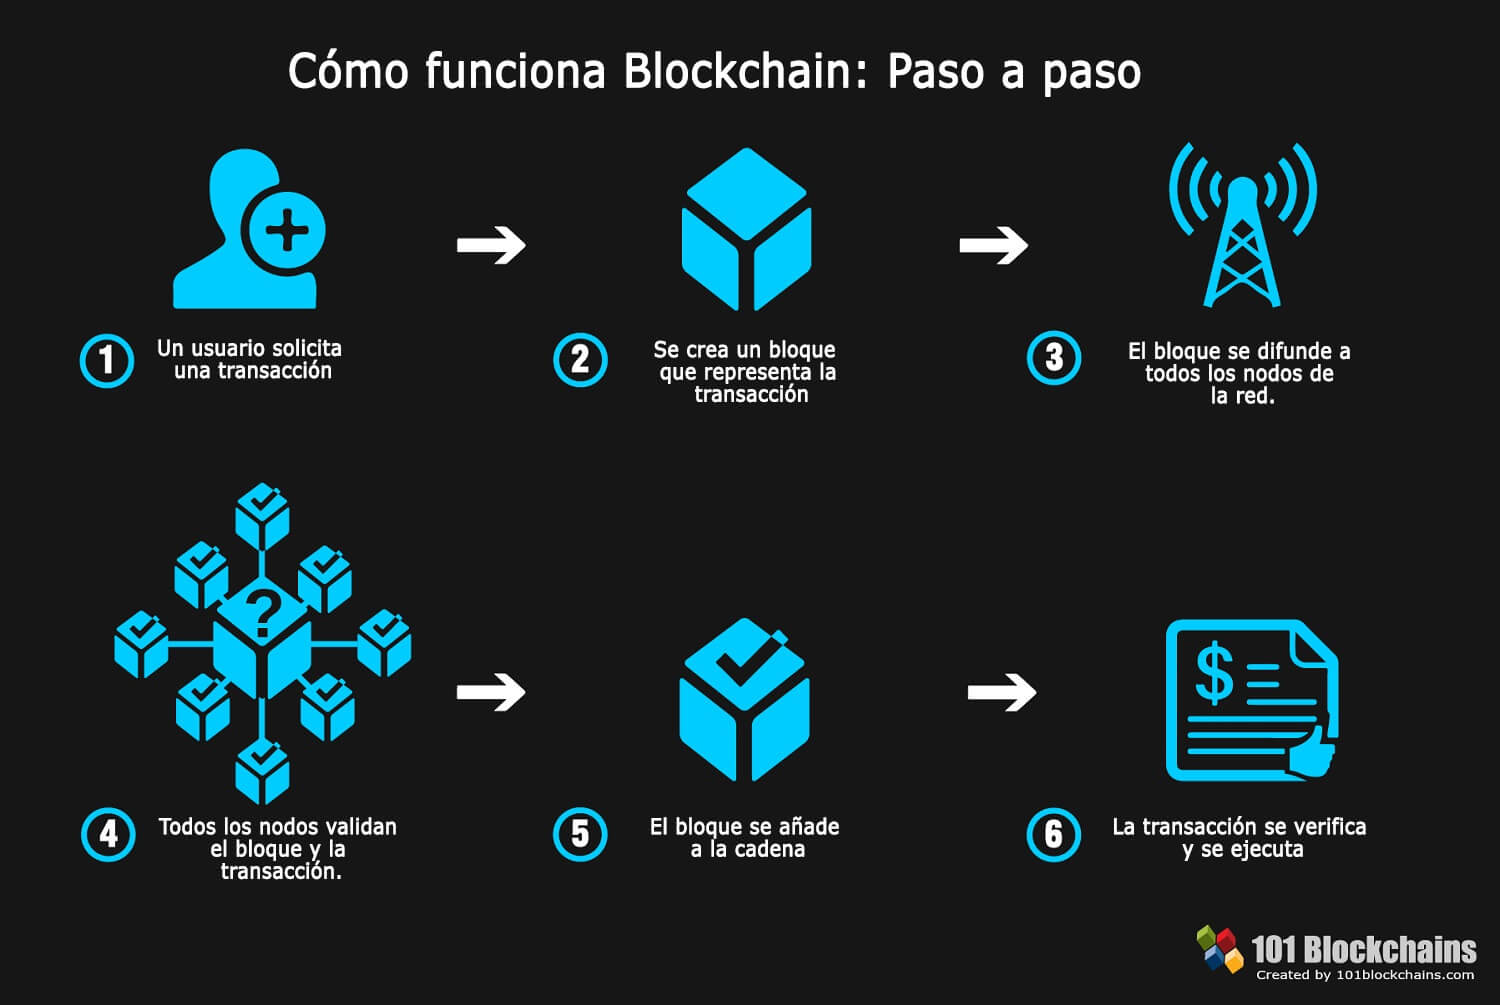
\includegraphics[width=0.8\textwidth,height=\textheight]{media/articulo01_image2.jpeg}}

\End{centerimageenv}

\Begin{smalltextenv}

\textbf{Imagen 1:} Gráfica del proceso de ingreso de un registro en blockchain. \textbf{Fuente:} \href{https://101blockchains.com/es/como-funciona-blockchain/}{101 Blockchains}

\End{smalltextenv}

\Begin{multicols}{2}

\spacefourmilis

La red de nodos es la arquitectura sobre la que toda esta tecnología está soportada; es una red de computadoras en la cual está replicada toda la cadena, es decir que cada nodo cuenta con una copia de la información. Cuando un bloque intenta ser alterado es fácilmente reconocido por los demás nodos de la red y por lo tanto, la información alterada pasa a ser inválida. Estos nodos son conocidos como ``mineros'' y su función, además de almacenar la información de la cadena, es que al momento de la creación de un nuevo bloque, deben intentar resolver un acertijo matemático que permita la generación de la ``huella''; esto con el fin de evitar una colisión de escritura entre los nodos debido a que es prácticamente imposible que dos nodos resuelvan el acertijo en el mismo momento.

\hypertarget{articulo01_cross01}{}

Durante estos años en Guatemala han existido proyectos que buscan utilizar esta tecnología para diversos fines, muchos de ellos han sido pruebas de concepto para demostrar cómo podría funcionar. Por ejemplo, en 2019 se realizó una subasta por parte de Anacafé con la colaboración de Yave, mediante la que se buscó acercar a los productores con los compradores a nivel internacional agilizando el proceso a través de la utilización de Blockchain, lo que permitiría la administración de transacciones sin necesidad de un ente centralizador, manteniendo estándares de seguridad sólidos. \protect\hyperlink{articulo01_ref01}{{[}1{]}}

\hypertarget{articulo01_cross02}{}

Otro proyecto que llamó la atención a nivel internacional fue ``Fiscal Digital''. Este proyecto buscaba utilizar Blockchain para facilitar la auditoría de la información gestionada en las elecciones de 2019. Para poder realizarlo obtuvieron del Tribunal Supremo Electoral las actas escaneadas enviadas por las juntas receptoras de votos, con las que generaron los códigos hash para luego registrarlas en una red de Blockchain, en este caso la de Bitcoin, con el fin de certificar su estado inicial y detectar, y evitar posibles modificaciones. Para reducir los costos de la utilización de dicha red utilizaron la herramienta OpenTimeStamp para generar árboles de Merklee y certificar las actas en grupos en lugar de hacerlo de manera individual. Además de esta utilización concreta de una cadena de bloques para la certificación de las imágenes de las actas también utilizaron el modelo conceptual del Blockchain para poder digitalizar la información contenida en dichas actas. Invitaron a usuarios externos a participar asumiendo el rol de mineros incentivando con premios a quienes digitaran más actas. La misma acta era digitada varias veces por distintas personas y la información era comparada entre las copias para verificar la veracidad de la información ingresada. En este caso lo ideal es que los votos se registren directamente en la cadena de bloques para obtener información de los votos en tiempo real y poder entregar resultados preliminares confiables rápidamente. \protect\hyperlink{articulo01_ref02}{{[}2{]}}

Debido a diversos factores en nuestro país, suele retrasarse algunos años la utilización de nuevas tecnologías en comparación con el resto del mundo. Sin embargo, empiezan a observarse proyectos que, aunque no busquen desarrollar un sistema propio de Blockchain, utilizan los sistemas existentes para poder aplicarlo en diversos sectores. En los siguientes años se espera que el gobierno y el sector privado se interesen más en la aplicación de esta tecnología debido los beneficios que conlleva para la sociedad coadyuvando a la solución de problemas nacionales.

\hypertarget{conclusiones}{%
\section*{Conclusiones}\label{conclusiones}}
\addcontentsline{toc}{section}{Conclusiones}

\begin{itemize}
\item
  Blockchain puede ser utilizado para muchas aplicaciones que requieran garantizar la fiabilidad de la información sin necesidad de la intervención de terceros.
\item
  Hasta el momento en Guatemala, la mayoría los proyectos de los que se tiene información han sido pruebas de concepto sobre cómo podría funcionar Blockchain, esperando que en un futuro se puedan explorar de mejor manera esta alternativa.
\end{itemize}

\hypertarget{referencias}{%
\section*{Referencias}\label{referencias}}
\addcontentsline{toc}{section}{Referencias}

\begin{itemize}
\item
  \hypertarget{articulo01_ref01}{}

  \protect\hyperlink{articulo01_cross01}{{[}1{]}} \href{https://republica.gt/}{«República»}, \href{https://republica.gt/2019/02/13/cafe-y-blockchain-anacafe-y-yave-inc-preparan-historica-subasta/}{¿Café y blockchain: Anacafé y Yave Inc.~preparan histórica subasta?}, 13 febrero 2019. {[}En línea{]}. Disponible en: \url{https://bit.ly/2BFEtcS}. {[}Último acceso: 12 marzo 2020{]}.
\item
  \hypertarget{articulo01_ref02}{}

  \protect\hyperlink{articulo01_cross02}{{[}2{]}} \href{https://ceiba.io}{«Ceiba»}, \href{https://ceiba.io/elecciones-generales-de-guatemala-2019-en-el-blockchain/}{Guatemala: El proceso electoral en Blockchain}, 28 enero 2020. {[}En línea{]}. Disponible en: \url{https://bit.ly/2De2Dvx}. {[}Último acceso: 12 marzo 2020{]}.
\end{itemize}

\End{multicols}

\titleformat{\chapter}[block]{\formatchapterEdDQ}{\labelchapterEdDQ}{170pt}{\beforecodechapterEdDQ#1\beforecodechapterparttwoEdDQ}

\titlespacing*{\chapter} {\leftchapterEdDQ}{\beforesepchapterEdDQDobleLine}{\afterchapterEdDQDobleLine}

\titleformat{\section}[block]{\formatsection}{\labelsection}{\sepsection}{\beforecodesection#1}

\titleformat{\subsection}[block]{\formatsubsection}{\labelsubsection}{\sepsubsection}{\beforecodesubsection#1}

\titleformat{\subsubsection}[block]{\formatsubsubsection}{\labelsubsubsection}{\sepsubsubsection}{\beforecodesubsubsection#1}

\hypertarget{article02}{%
\chapter{Qué es la transformación digital y cuál es su importancia}\label{article02}}

\BeginKnitrBlock{photobiography3}{media/articulo02_image1.png}
\begin{styleAuthorName}

Dénilson Eduardo Argueta Higueros

\end{styleAuthorName}

\begin{styleAuthormail}

\textbf{\href{mailto:deahtom123@gmail.com}{\nolinkurl{deahtom123@gmail.com}}}

\end{styleAuthormail}

Estudiante de Ingeniería en Ciencias y Sistemas - USAC

\begin{styleKeywords}

\textbf{Palabras Clave:}\\
\emph{Transformación}, \emph{digital}, tecnología, empresas.

\end{styleKeywords}
\EndKnitrBlock{photobiography3}

\Begin{multicols}{2}

\spaceminusmilis

La transformación digital es un concepto con el que no está familiarizado todo el mundo. Quizá porque es un concepto reciente, pero es algo que lleva mucho tiempo aplicándose en los negocios. La transformación digital se define como la renovación del modelo de negocio que tiene alguna empresa; es cuando se utilizan nuevas tecnologías para mejorar el funcionamiento de la empresa y alcanzar más personas. Es importante también para lograr la optimización de los procesos, para ahorrar recursos, ser eficaces, ofrecer nuevos servicios a los clientes y competir con negocios similares. En otros términos, la transformación digital consiste en la transformación de los modelos de negocios de la empresa como: manejar ventas en línea, servicio al cliente en línea, etc. Se trata que la empresa pueda llegar a muchas más personas obteniendo una comunicación más directa con los clientes.
\spaceminusmilis
Muchas empresas que digitalizan los procesos han tenido éxito en comparación de aquellas que no lo han hecho. Las primeras tienen mayor número de clientes que las otras empresas y lo que se traduce en más ganancias. Esto se debe a que los clientes se sienten más cómodos comprando, pagando, preguntando, etc. en línea y desde la comodidad de su casa, ya que esto les ahorra tiempo y dinero con solo un clic desde su hogar.

\Begin{centerimageenv}

\href{https://www.blog.andaluciaesdigital.es/wp-content/uploads/2017/05/1024x512transformaciondigital.png}{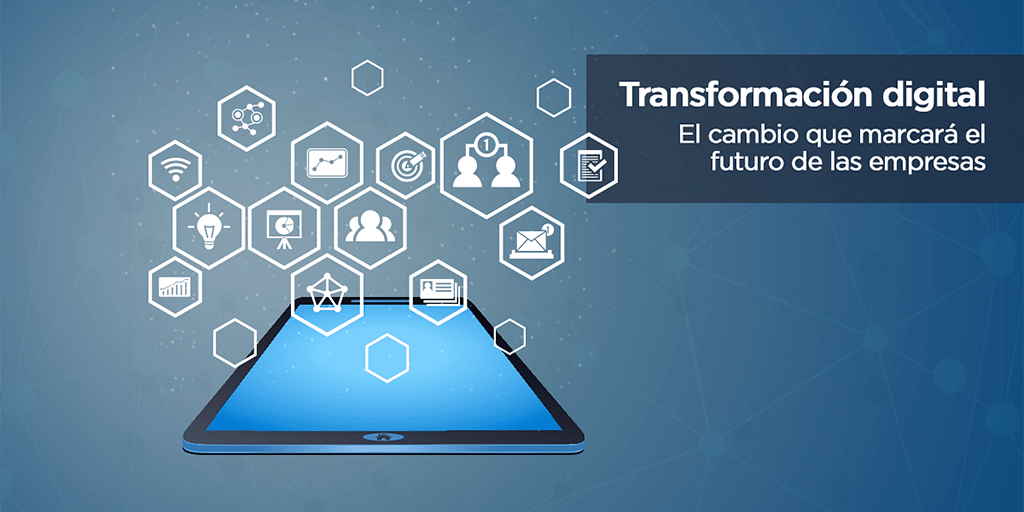
\includegraphics[width=0.45\textwidth,height=\textheight]{media/articulo02_image2.png}}

\End{centerimageenv}

\Begin{smalltextenv}

\textbf{Imagen 1:} Dispositivo móvil y algunos símbolos para representar tecnología. \textbf{Fuente:} \href{https://www.blog.andaluciaesdigital.es/wp-content/uploads/2017/05/1024x512transformaciondigital.png}{\emph{Andalucía es digital}}

\End{smalltextenv}

\spaceminusmilis

Por ejemplo: la mayoría de las personas prefieren ver y rentar una película desde la comodidad de su casa que salir a comprar o alquilar una película, o pagar el recibo de la luz en línea y en vez de ir al banco a realizar el pago haciendo largas colas y perdiendo tiempo.

\spaceminusmilis

\hypertarget{articulo02_cross02}{}
\hypertarget{articulo02_cross03}{}

Para la mayor parte de las empresas la transfor-
mación digital ya no es una opción. Las empresas que no se han digitalizado han perdido terreno y oportunidades de negocios en comparación con las empresas que se han digitalizado y muchas han ido a la bancarrota debido a esto. Las empresas tienen más oportunidades de llegar al éxito si realizan una transformación digital en el modelo de negocio. Muchas empresas tienen miedo de realizar una transformación digital ya sea por desconocimiento o por miedo de tener toda la información importante de forma digital, porque creen que será un proceso muy caro e inseguro, pero eso es un proceso que se debe realizar a mediano o largo plazo. En sí deben analizar el impacto que tendrán en el mercado transformándose digitalmente y las ventajas que tendrán su empresa al realizarla. Uno de los ejemplos con el que puede entenderse mejor la importancia de la transformación digital es a través del ejemplo de Blockbuster y Netflix \protect\hyperlink{articulo02_ref02}{{[}2{]}}. En el pasado Blockbuster lideraba el mercado de películas, cualquier persona que rentaba una película debía ir a la tienda, rentaba la película por un tiempo y luego la devolvía. Netflix cambio totalmente el modelo de negocio de rentar películas. Los creadores de Netflix desarrollaron una plataforma en donde las personas ven las películas en línea sin límites en cuanto a la cantidad de películas a rentar. Netflix tiene un catálogo de películas y series donde puede verse cualquier película del catálogo en cualquier momento y en cualquier dispositivo. Netflix tomó el liderazgo de películas y series en todo el mundo. Ofrecen una gran variedad de películas sin necesidad de salir de casa; se puede disfrutar del contenido que ofrecen a un precio accesible. El gran éxito de Netflix llevó a la bancarrota a Blockbuster y a otros competidores en el mercado.

\Begin{centerimageenv}

\href{https://i.blogs.es/d4dbcb/netflix1/1366_2000.jpg}{
\includegraphics[width=0.45\textwidth,height=\textheight]{media/articulo02_image3.jpeg}}

\End{centerimageenv}

\Begin{smalltextenv}

\textbf{Imagen 2:} Dominio de Netflix sobre Blockbuster \textbf{Fuente:} \href{https://www.xataka.com/cine-y-tv/nadie-se-acuerda-blockbuster-tuvo-a-netflix-cuerdas-pudo-comprar-50-millones-dolares}{Xataka}

\End{smalltextenv}

\spaceminusmilis

A raíz del éxito de Netflix muchas empresas le han apostado al negocio de contenidos por streaming y la mayoría de estas han tenido éxito como HBO, Disney, Amazon, etc. Entre los beneficios que han traído estas plataformas están: ahorro en tiempo y dinero al no tener que salir de casa para rentar una película/serie; la forma de buscar el contenido es mucho más sencillo ya que en las plataformas se puede buscar por género, por actor, nombre, etc. lo cual facilita al usuario a elegir el contenido deseado; las series y películas se pueden disfrutar desde cualquier dispositivo, se puede ver en celulares, tabletas, computadoras, televisores, etc. Se puede pausar el contenido y seguir viendo desde donde se pausó en otro dispositivo; y también pueden ver varias personas contenidos diferentes al mismo tiempo. Así como se dio el caso de Netflix y Blockbuster han existido muchos casos similares en donde las empresas que han cambiado el modelo de negocio han triunfado y han hecho que las empresas que ofrecen un producto similar vayan a la quiebra.

\spaceminusmilis

Otro ejemplo es el caso de Amazon y Sears \protect\hyperlink{articulo02_ref03}{{[}3{]}} en donde Amazon cambió el modelo de negocio de la venta de artículos ya que siempre se vendían en tiendas locales y Amazon se enfocó en las ventas en línea a nivel mundial. Amazon mejoró el modelo de ventas y aumentó sus ganancias exponencialmente dejando a SEARS en la bancarrota.

\spaceminusmilis

Las claves para lograr exitosamente la transfor-
mación digital son: mejorar la experiencia del cliente dándole soporte en línea; creando sitios web en donde el usuario pueda encontrar la información que necesita; y creando aplicaciones o páginas que puedan ser accedidas desde cualquier dispositivo. Toda la información que se almacena de los negocios es importante que se encuentre en línea para que pueda ser accedida desde cualquier parte y pueda ser accedida concurrentemente.

\spacefivemilis

Es importante manejar muchas estrategias digitales para llegar a más personas. Algunas de estas estrategias son: por medio de publicidad o con una comunicación más personalizada con los clientes, tales como: llamadas, correos o chats para brindar mejor servicio a los clientes. También es importante cambiar la visión del entorno y apostar por algo que los vuelva diferentes a las demás empresas que ofrezcan el mismo producto.

\spacefivemilis

La transformación digital trae como ventajas generar nuevas experiencias al cliente, generar nuevas y más fuentes de ingreso, se impulsa a tener una cultura de innovación y como consecuencia hará que los empleados opten por nuevas ideas que mejoren el negocio. También mejorará la eficiencia de operación lo que redundará en servicios o productos de mejor calidad para el cliente en un corto tiempo.

\spaceeightmilis

\Begin{centerimageenv}

\href{http://web.sigmma.net/elsiglo/sitio/uploads/notas/transformacion-digital.jpg}{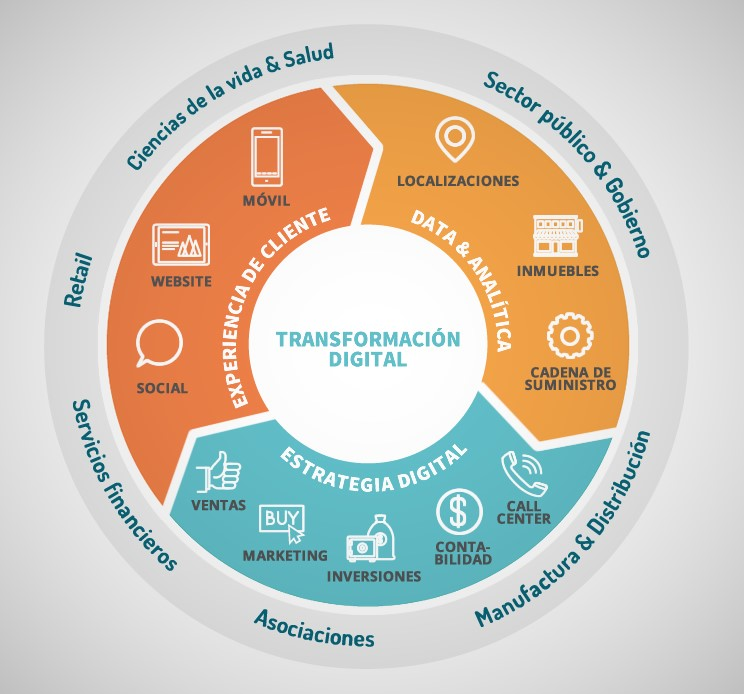
\includegraphics[width=0.45\textwidth,height=\textheight]{media/articulo02_image4.jpeg}}

\End{centerimageenv}

\Begin{smalltextenv}

\textbf{Imagen 2:} Representación gráfica de lo que consiste la transformación digital. \textbf{Fuente:} \href{http://web.sigmma.net/nota/373/qu-es-la-transformacin-digital-para-una-agencia-de-viajes.html}{Sigmma}

\End{smalltextenv}

\spacefivemilis

\hypertarget{conclusiones-1}{%
\section*{Conclusiones}\label{conclusiones-1}}
\addcontentsline{toc}{section}{Conclusiones}

\begin{itemize}
\tightlist
\item
  Si las empresas no evolucionan con las nuevas tecnologías, tienen alta probabilidad de desaparecer.
  \spacefourmilis
\item
  La transformación digital consiste en la transfor-
  mación de los modelos de negocios de la empresa la cual trae muchos beneficios a los negocios.
  \spacefourmilis
\item
  Muchas empresas temen realizar una transfor-
  mación digital ya sea por desconocimiento o por miedo de tener toda la información importante de forma digital o porque creen que será un proceso muy caro e inseguro.
  \spacefourmilis
\item
  La transformación digital no es posible si no se integran correctamente los recursos tecnológicos en todas las áreas de la empresa.
\end{itemize}

\spacefivemilis

\hypertarget{referencias-1}{%
\section*{Referencias}\label{referencias-1}}
\addcontentsline{toc}{section}{Referencias}

\begin{itemize}
\item
  \hypertarget{articulo02_ref01}{}

  {[}1{]} \href{https://www.ttandem.com/}{«Planeta ttandem»}, \href{https://www.ttandem.com/blog/que-es-la-transformacion-digital-y-por-que-es-necesaria-para-cualquier-negocio}{Qué es la transformación digital y por qué es necesaria para cualquier negocio}, 09 marzo 2020. {[}En línea{]}. Disponible en: \url{https://bit.ly/2ClMdAS}. {[}Último acceso: 09 marzo 2020{]}.
\item
  \hypertarget{articulo02_ref02}{}

  \protect\hyperlink{articulo02_cross02}{{[}2{]}} \href{http://www.xataka.com/}{«Xataka»}, \href{https://www.xataka.com/cine-y-tv/nadie-se-acuerda-blockbuster-tuvo-a-netflix-cuerdas-pudo-comprar-50-millones-dolares/}{Blockbuster tuvo a Netflix contra las cuerdas: la pudo comprar por 50 millones de dólares}, 29 julio 2019. {[}En línea{]}. Disponible en: \url{https://bit.ly/2ZiRC4s}. {[}Último acceso: 09 marzo 2020{]}.
\item
  \hypertarget{articulo02_ref03}{}

  \protect\hyperlink{articulo02_cross03}{{[}3{]}} \href{https://www.lainformacion.com/}{«La Información»}, \href{https://www.lainformacion.com/empresas/el-gigante-estadounidense-sears-se-rinde-ante-amazon-y-se-declara-en-bancarrota/6434093/}{El gigante estadounidense Sears se rinde ante Amazon y se declara en bancarrota}, 15 octubre 2018. {[}En línea{]}. Disponible en: \url{https://bit.ly/3iVGnHa}. {[}Último acceso: 09 marzo 2020{]}.
\end{itemize}

\End{multicols}

\Begin{centerimageenv}

\href{https://www.usac.edu.gt}{
\includegraphics[width=1\textwidth,height=\textheight]{media/articulo02_image5.png}}

\End{centerimageenv}

\Begin{centerimageenv}

\href{https://dtt-ecys.org}{
\includegraphics[width=0.25\textwidth,height=\textheight]{media/logo_50.png}}

\End{centerimageenv}

\titleformat{\chapter}[block]{\formatchapterEdDQ}{\labelchapterEdDQ}{195pt}{\beforecodechapterEdDQ#1\beforecodechapterparttwoEdDQ}

\titlespacing*{\chapter} {\leftchapterEdDQ}{\beforesepchapterEdDQDobleLine}{\afterchapterEdDQDobleLine}

\titleformat{\section}[block]{\formatsection}{\labelsection}{\sepsection}{\beforecodesection#1}

\titleformat{\subsection}[block]{\formatsubsection}{\labelsubsection}{\sepsubsection}{\beforecodesubsection#1}

\titleformat{\subsubsection}[block]{\formatsubsubsection}{\labelsubsubsection}{\sepsubsubsection}{\beforecodesubsubsection#1}

\hypertarget{article03}{%
\chapter{Sistemas Operativos: pasado, actualidad y, ¿olvido?}\label{article03}}

\BeginKnitrBlock{photobiography3}{media/articulo03_image1.png}
\begin{styleAuthorName}

Alan Giovanni Guzmán Toledo

\end{styleAuthorName}
\begin{styleAuthormail}

\textbf{\href{mailto:haldamir.95@gmail.com}{\nolinkurl{haldamir.95@gmail.com}}}

\end{styleAuthormail}

Estudiante de Ingeniería en Ciencias y Sistemas - USAC

\begin{styleKeywords}

\textbf{Palabras Clave:}\\
Sistemas Operativos, hardware, software, serverless, lenguaje máquina.

\end{styleKeywords}
\EndKnitrBlock{photobiography3}

\Begin{multicols}{2}

Transcurría la cuarta década del siglo XX cuando a raíz de la segunda guerra mundial se desarrolló la informática. En esos años no existía el concepto de sistema operativo y los programadores debían de comunicarse directamente con el hardware. La comunicación entre el humano y la máquina se daba a través de un lenguaje simple de entender pero muy complejo de utilizar. Este lenguaje es denominado ``lenguaje máquina'', que no es más que un código binario; es decir, por esa época programaban utilizando ceros y unos.

\spacefourmilis

El concepto de ``Sistema Operativo'' surgió en la década de los años 50 debido al nacimiento de varios circuitos que manejaban el hardware de forma automática. El primer sistema operativo que interactuó de manera más amigable con el humano fue creado en 1954 dándole vida así a una computadora IBM 704. Su nombre fue Atlas Supervisor y era capaz de ejecutar programas en un lenguaje de alto nivel llamado FORTRAN.

\spaceminusmilis

Este tipo de sistemas operativos se reprodujeron a lo largo del tiempo y evolucionaron velozmente. Los sistemas operativos y las computadoras eran totalmente empresariales y su uso y dominio eran muy complejos. Estos sistemas estaban al alcance únicamente de personal muy cualificado y su operabilidad conllevaba un alto consumo de recursos. Los sistemas operativos más utilizados en esa década fueron UNIX, MULTICS, BDOS y CP/M. En los años 80, la humanidad fue estremecida con la llegada de las computadoras personales, llegando a oficinas y miles de hogares, pero lograr esto no fue sencillo debido a que, como se mencionara, los sistemas operativos eran únicamente para expertos en la materia. Gracias a la llegada de las computadoras personales surgieron los sistemas operativos tal y como se conocen hoy, más amigables con los usuarios, y con la integración de elementos gráficos como los menús. Entre los sistemas operativos más utilizados y ahora legendarios están Mac OS, GNU/Linux, Solaris y Microsoft Windows.

\End{multicols}

\Begin{centerimageenv}

\href{http://images.computerhistory.org/revonline/images/102641445-03-01.jpg?w=600}{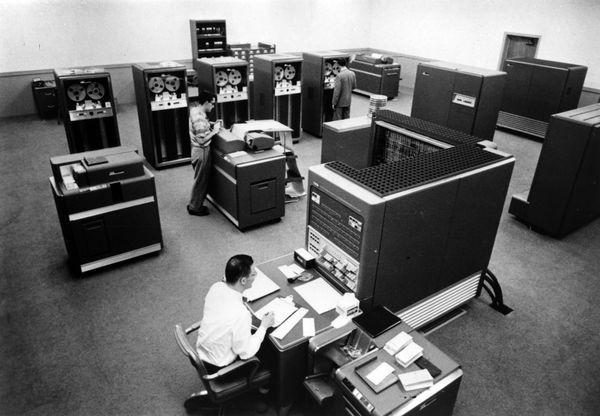
\includegraphics[width=0.55\textwidth,height=\textheight]{media/articulo03_image2.jpeg}}

\End{centerimageenv}

\Begin{smalltextenv}

\textbf{Imagen 1:} Computadora IBM 704 siendo programada en FORTRAN. \textbf{Fuente:} \href{https://computerhistory.org/}{© International Business Machines Corporation (IBM)}

\End{smalltextenv}

\Begin{multicols}{2}
\spaceminusmilis

Hasta ahora se ha mencionado como surgieron los sistemas operativos, como evolucionaron y se adaptaron a las necesidades de los usuarios, habiéndose comprendido la importancia de los sistemas operativos a lo largo de la historia y el importante papel de estos como herramienta de trabajo. Habiendo reseñado lo asombrosos e importantes que son los sistemas operativos, surgen preguntas tales como: ¿Cuándo fue la última vez que un usuario se interesó en el funcionamiento del sistema operativo? ¿Realmente se está utilizando el sistema operativo ideal para las necesidades reales? Y de no ser el caso ¿hay disposición para buscar un sistema operativo ideal para y empezar a utilizarlo?
\spaceminusmilis
En lo personal, como estudiante de ingeniería en ciencias y sistemas me hago otro tipo de preguntas que también dirijo a mis colegas y superiores: ¿Es el sistema operativo que utilizo un ambiente de desarrollo adecuado a mis exigencias? ¿Debería reparar en detalles de los sistemas operativos que utilizará mi arquitectura de software? En la actualidad existen tecnologías asombrosas como la arquitectura Serverless en la cual se delega todo el trabajo de infraestructura y hardware al proveedor mientras que el usuario solamente tiene cuidado del código de la aplicación.

\Begin{centerimageenv}

\href{https://upload.wikimedia.org/wikipedia/commons/e/e3/Macintosh_128k_transparency.png}{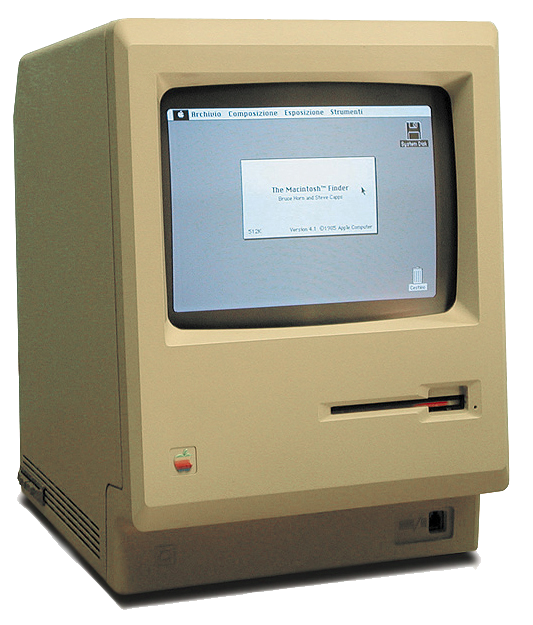
\includegraphics[width=0.2\textwidth,height=\textheight]{media/articulo03_image3.png}}

\End{centerimageenv}

\Begin{smalltextenv}

\textbf{Imagen 2:} Computadora Macintosh 128k con el sistema operativo ``System 1'' o también llamado ``Classic Mac OS''. \textbf{Fuente:} \href{https://es.wikipedia.org/wiki/Macintosh/}{Wikipedia}

\End{smalltextenv}

Poco a poco los sistemas operativos pasaron de ser el centro de atención a volverse una herramienta trivial y transparente que siempre existe alrededor. De alguna manera se puede pensar que los desarrolladores de sistemas operativos, ya sean sistemas open source o no, tienen un lado altruista al querer seguir mejorando esta magnífica herramienta, aunque no se les reconozca o se admire su trabajo. De igual modo, los sistemas operativos siempre van a estar disponibles para cualquier tipo de usuario, aunque surjan incomodidades por fallos o por actualizaciones inesperadas. Aunque ya no sea objeto de aprecio como antes, aunque no se busque entender cómo funcionan y aunque pasen desapercibidos a los ojos de muchos, los sistemas operativos siempre estarán allí, en las tareas, en la universidad, en la oficina, e incluso en la NASA, los sistemas operativos serán fieles colaboradores aun estando en el baúl del olvido.

\hypertarget{articulo03_cross03}{}

``Algunas cosas se hacen tan nuestras que las olvidamos'' \protect\hyperlink{articulo03_ref03}{{[}3{]}}

\spaceminusmilis

\hypertarget{conclusiones-2}{%
\section*{Conclusiones}\label{conclusiones-2}}
\addcontentsline{toc}{section}{Conclusiones}

\begin{itemize}
\item
  Los sistemas operativos son elementos impor-
  tantes en el día a día de la mayoría de personas y debiera tenerse la capacidad de entenderlos y distinguirlos según sus características para la satisfacción de necesidades.
\item
  Las nuevas tecnologías buscan hacer más fácil el trabajo de los desarrolladores y arquitectos de software, sin embargo, aunque parezca que los sistemas operativos ya no son una variable en la ecuación, siempre van a estar presentes y su trabajo será más que fundamental para el éxito.
\item
  Todas las personas deberían de tener conoci-
  mientos básicos del funcionamiento de los sistemas operativos y su importancia, mientras que quienes estudian informática debieran ser capaces de interactuar más a fondo con el sistema operativo y poder explotarlo de manera adecuada para mejorar altamente el rendimiento laboral.
\end{itemize}

\spaceminusmilis

\hypertarget{referencias-2}{%
\section*{Referencias}\label{referencias-2}}
\addcontentsline{toc}{section}{Referencias}

\begin{itemize}
\item
  \hypertarget{articulo03_ref01}{}

  {[}1{]} \href{https://es.wikipedia.org/}{«Wikipedia»}, \href{https://es.wikipedia.org/wiki/Historia_de_los_sistemas_operativos}{Historia de los sistemas operativos}, 15 octubre 2003. {[}En línea{]}. Disponible en: \url{https://bit.ly/3euZiF9}. {[}Último acceso: 10 marzo 2020{]}.
\item
  \hypertarget{articulo03_ref02}{}

  {[}2{]} \href{https://en.wikipedia.org/}{«Wikipedia»}, \href{https://en.wikipedia.org/wiki/Timeline_of_operating_systems}{Timeline of operating systems}, 17 junio 2003. {[}En línea{]}. Disponible en: \url{https://bit.ly/2OrU2HW}. {[}Último acceso: 10 marzo 2020{]}.
\item
  \hypertarget{articulo03_ref03}{}

  \protect\hyperlink{articulo03_cross03}{{[}3{]}} Antonio Porchia (2017). \emph{Voces}, Buenos Aires, Argentina: Luces Galibo.
\end{itemize}

\End{multicols}

\titleformat{\chapter}[block]{\formatchapterEdDQ}{\labelchapterEdDQ}{\sepchapterEdDQ}{\beforecodechapterEdDQ#1\beforecodechapterparttwoEdDQ}

\titlespacing*{\chapter} {\leftchapterEdDQ}{\beforesepchapterEdDQ}{\afterchapterEdDQ}

\titleformat{\section}[block]{\formatsection}{\labelsection}{\sepsection}{\beforecodesection#1}

\titleformat{\subsection}[block]{\formatsubsection}{\labelsubsection}{\sepsubsection}{\beforecodesubsection#1}

\titleformat{\subsubsection}[block]{\formatsubsubsection}{\labelsubsubsection}{\sepsubsubsection}{\beforecodesubsubsection#1}

\hypertarget{article04}{%
\chapter{El Internet para todos}\label{article04}}

\BeginKnitrBlock{photobiography3}{media/articulo04_image1.png}
\begin{styleAuthorName}

Noé Alfonso Ruiz Rivera

\end{styleAuthorName}
\begin{styleAuthormail}

\textbf{\href{mailto:noetux7@gmail.com}{\nolinkurl{noetux7@gmail.com}}}

\end{styleAuthormail}

Estudiante de Ingeniería en Ciencias y Sistemas - USAC

\begin{styleKeywordsTwo}

\textbf{Palabras Clave:}\\
Internet, StarLink, SpaceX, Amazon, Blue Origin, Google Loon, satélite.

\end{styleKeywordsTwo}
\EndKnitrBlock{photobiography3}

\Begin{multicols}{2}

\hypertarget{articulo04_cross01}{}
\hypertarget{articulo04_cross02}{}
\spacefourmilis

El acceso a Internet es cada vez más común en todo el mundo, sin embargo, aún existe un gran porcentaje de la población mundial que no tiene acceso a la red global. Muchas personas accedemos con frecuencia a la Internet, tanto que es parte de nuestra rutina diaria. Esto ha creado una brecha en el acceso a la información, las personas que no tienen acceso están en desventaja frente a las que sí. En varios países no se trata únicamente del acceso a Internet sino de la censura y falta de libertad que tienen sus ciudadanos en la red. Países como China, Irán y Corea del Norte tienen completo control de sus ciudadanos y les limitan sus libertades. Ahora podemos entender por qué las Naciones Unidas declararon que el acceso a Internet y la libertad en él es un derecho humano en su resolución A/HRC/32/L.20 \protect\hyperlink{articulo04_ref01}{{[}1{]}}.

\spacefivemilis

\Begin{centerimageenv}

\href{https://wearesocial-net.s3.amazonaws.com/es/wp-content/uploads/sites/12/2020/01/01-Global-Overview-\%E2\%80\%93-DataReportal-Digital-2020-Global-Digital-Overview-Slide-8.png}{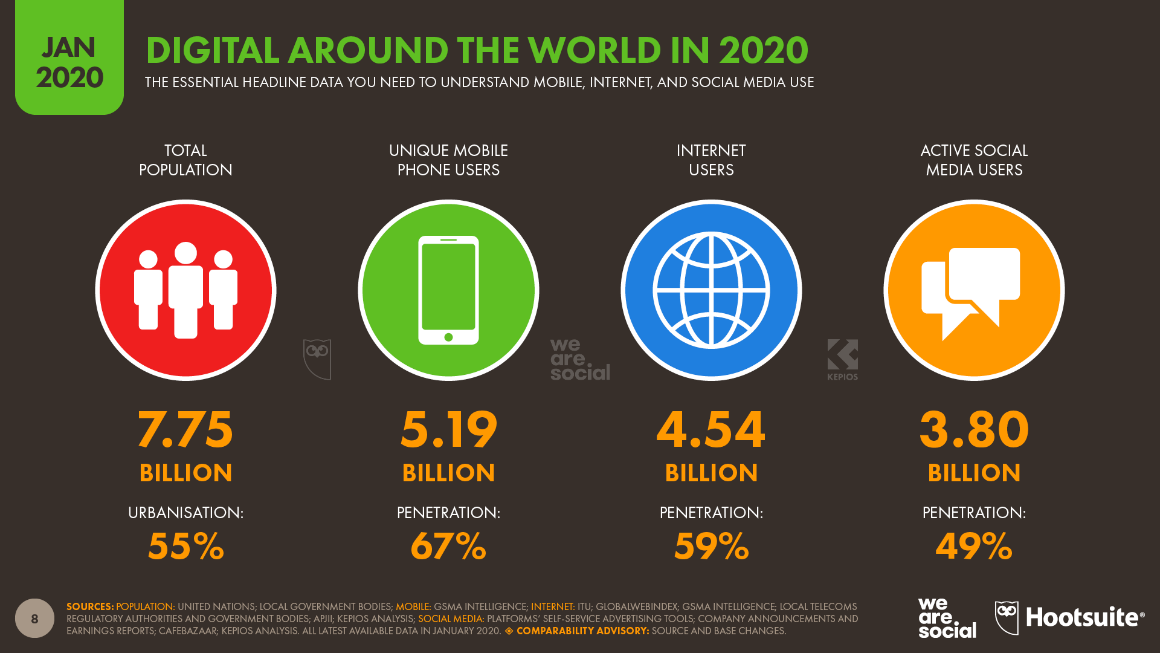
\includegraphics[width=0.48\textwidth,height=\textheight]{media/articulo04_image2.png}}

\End{centerimageenv}

\Begin{smalltextenv}

\textbf{Imagen 1:} Digital around the world in 2020. \textbf{Fuente:} \href{https://wearesocial.com/es/blog/2020/01/digital-2020-el-uso-de-las-redes-sociales-abarca-casi-la-mitad-de-la-poblacion-mundial}{WeAreSocial}

\End{smalltextenv}

\spacefivemilis

El acceso a Internet actualmente se ha facilitado más gracias a los dispositivos móviles y los avances tecnológicos en el área de las redes inalámbricas. Este progreso ha permitido que más personas estén en comunicación a través de sus dispositivos móviles y redes sociales \protect\hyperlink{articulo04_ref02}{{[}2{]}}.

\spacefivemilis

Durante la última década diversas empresas se han interesado más en cerrar está brecha. La falta de acceso a Internet puede tomarse como un problema de desigualdad social, ya que es considerado un derecho humano. Empresas como Google, SpaceX o Amazon lo ven como una oportunidad de negocio.

\hypertarget{articulo04_cross03}{}
\spacefivemilis

Una de las primeras empresas en proponer una solución a este problema fue Google en 2013 con su proyecto Loon. Este proyecto consiste en la utilización de globos de helio colocados en la estratósfera, a unos 20 kilómetros, y más recientemente con el uso de drones. Sus globos funcionan con energía solar y emiten señal 4G o 5G cubriendo un diámetro de 80 kilómetros\protect\hyperlink{articulo04_ref03}{{[}3{]}}. Su programa piloto fue probado en Nueva Zelanda, actualmente ya se han hecho pruebas en algunas zonas de países como Brasil, Australia, Perú y Sudáfrica. Más recientemente el proyecto Loon ha adaptado esta tecnología, en conjunto con otras empresas, a drones los cuales permiten conexión hasta 700 kilómetros y velocidad de hasta 1Gbps.

\Begin{centerimageenv}

\href{https://commons.wikimedia.org/wiki/File:Google_Loon_-_Launch_Event.jpg}{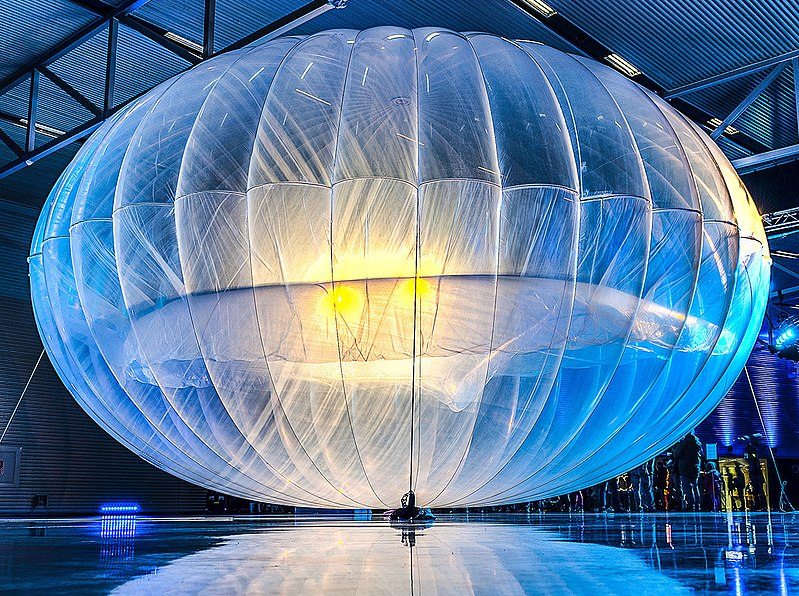
\includegraphics[width=0.48\textwidth,height=\textheight]{media/articulo04_image3.jpeg}}

\End{centerimageenv}

\Begin{smalltextenv}

\textbf{Imagen 2:} Globo de Loon en el evento de lanzamiento en junio de 2013. \textbf{Fuente:} \href{https://elpais.com/elpais/2018/07/24/planeta_futuro/1532414715_476889.html}{ElPais}

\End{smalltextenv}

\hypertarget{articulo04_cross04}{}

\spacefivemilis

Amazon es una de las empresas más grandes del mundo, por lo cual tiene recursos de sobra para realizar un proyecto tan ambicioso como lo es llevar internet a todo el mundo, sin mencionar que su fundador también es dueño de Blue Origin, una empresa aeroespacial. Su proyecto Kuiper tiene planeado enviar 3,236 satélites para formar una constelación que lleve internet a gran parte del planeta, esperando tener una cobertura del 95\% de la población mundial \protect\hyperlink{articulo04_ref04}{{[}4{]}}. Este proyecto aún está en planeación y están dispuestos a hacer alianzas con otras empresas para alcanzar su objetivo. Pero Amazon no es la única empresa con estos planes, OneWeb, una empresa de telecomunicaciones también tiene planeado lanzar 650 satélites para proveer de señal WiFi, LTE y 3G. Facebook también ha anunciado que está trabajando en este tipo de proyectos.

\spacefivemilis
\hypertarget{articulo04_cross05}{}

Hasta el momento todas estas propuestas y pruebas experimentales que han hecho las compañías ya mencionadas resultan muy interesantes y prometedoras, sin embargo, existe una compañía que va mucho más adelantada que todas las demás, se trata de SpaceX. El proyecto Starlink consiste en una red o constelación de satélites que son puestos en órbita por SpaceX, el objetivo como en todas las empresas con este tipo de programas es el de llevar internet de bajo costo a todo el mundo. Se tiene planeada una red de 12,000 satélites. El proyecto Starlink fue anunciado por primera vez en enero 2015, a diferencia de sus competidores SpaceX ha avanzado mucho con este proyecto y ya ha lanzado varias cadenas de satélites sin mencionar que ya tiene los permisos necesarios para enviar los 12,000 satélites de su plan preliminar \protect\hyperlink{articulo04_ref05}{{[}5{]}}.

\spacefivemilis

Luego de lanzar 2 satélites de prueba SpaceX lanzó sus primeros 60 satélites de Starlink el 23 de mayo de 2019, utilizó el cohete Falcon 9 para esta misión, colocándolos a una altitud de 550 kilómetros. Luego de esto SpaceX ha realizado varias misiones exitosas llevando a órbita 60 satélites en cada una de ellas. Su servicio ya está realizando pruebas en EE. UU. y Canadá.

\Begin{centerimageenv}

\href{https://commons.wikimedia.org/wiki/File:Starlink_SpaceX_1584_satellites_72_Planes_22each.png}{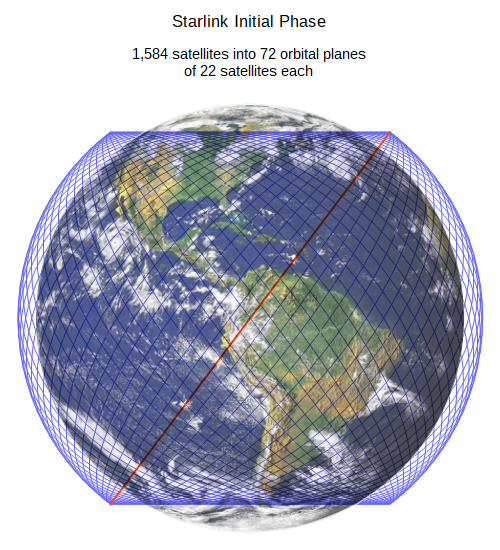
\includegraphics[width=0.45\textwidth,height=\textheight]{media/articulo04_image4.png}}

\End{centerimageenv}

\Begin{smalltextenv}

\textbf{Imagen 3:} Planificación de la constelación de satélites para la primera fase de Starlink. \textbf{Fuente:} \href{https://elpais.com/elpais/2018/07/24/planeta_futuro/1532414715_476889.html}{Wikimedia}

\End{smalltextenv}

\spacefivemilis

SpaceX sabe que la cantidad de satélites que utilizarán para este proyecto es enorme y los satélites que dejen de funcionar se convertirán en basura espacial, un problema para otros satélites, por lo cual la órbita de 550 km hará que estos satélites se consuman completamente en un periodo de 1 a 5 años en caso de que queden inoperables.

\spacefivemilis

\Begin{centerimageenv}

\href{https://commons.wikimedia.org/wiki/File:Starlink_Mission_(47926144123).jpg}{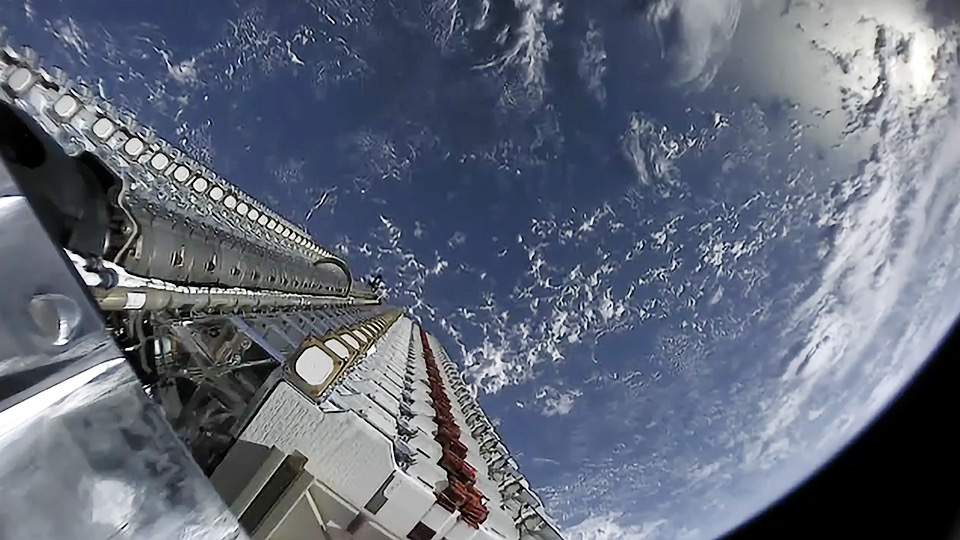
\includegraphics[width=0.48\textwidth,height=\textheight]{media/articulo04_image5.jpeg}}

\End{centerimageenv}

\Begin{smalltextenv}

\textbf{Imagen 4:} 60 satélites Starlink en un Falcon 9 listos para ponerse en órbita. \textbf{Fuente:} \href{https://www.space.com/spacex-starlink-satellites.html}{Official SpaceX Photos}

\End{smalltextenv}

\spacefivemilis

\hypertarget{conclusiones-3}{%
\section*{Conclusiones}\label{conclusiones-3}}
\addcontentsline{toc}{section}{Conclusiones}

\begin{itemize}
\item
  El acceso a Internet se ha convertido en un servicio básico en nuestra sociedad, las personas que no tienen acceso están en desventaja. El acceso a Internet resulta ser ahora un derecho humano.
\item
  La tarea de llevar Internet a cada rincón del planeta es compleja y costosa, por ello solo las grandes empresas del mundo pueden competir en este ámbito.
\item
  SpaceX es la empresa que lleva más avances con su proyecto Starlink, ya ha realizado varias misiones para poner en órbita sus satélites e incluso son visibles a simple vista desde la tierra.
\end{itemize}

\hypertarget{referencias-3}{%
\section*{Referencias}\label{referencias-3}}
\addcontentsline{toc}{section}{Referencias}

\begin{itemize}
\item
  \hypertarget{articulo04_ref01}{}

  \protect\hyperlink{articulo04_cross01}{{[}1{]}} \href{https://www.businessinsider.com/}{«Businessinsider»}, \href{https://www.businessinsider.com/un-says-internet-access-is-a-human-right-2016-7}{UN thinks internet access is a human right}, 22 julio 2016. {[}En línea{]}. Disponible en: \url{https://bit.ly/2Cr05tV}. {[}Último acceso: 11 marzo 2020{]}.
\item
  \hypertarget{articulo04_ref02}{}

  \protect\hyperlink{articulo04_cross02}{{[}2{]}} \href{https://wearesocial.com/}{«WeAreSocial»}, \href{https://wearesocial.com/es/blog/2020/01/digital-2020-el-uso-de-las-redes-sociales-abarca-casi-la-mitad-de-la-poblacion-mundial}{Digital 2020: el uso de las redes sociales abarca casi la mitad de la población mundial}, 30 enero 2020. {[}En línea{]}. Disponible en: \url{https://bit.ly/2WypWqz}. {[}Último acceso: 11 marzo 2020{]}.
\item
  \hypertarget{articulo04_ref03}{}

  \protect\hyperlink{articulo04_cross03}{{[}3{]}} \href{https://elpais.com/}{«ElPais»}, \href{https://elpais.com/elpais/2018/07/24/planeta_futuro/1532414715_476889.html}{Globos para llevar Internet al fin del mundo}, 30 enero 2020. {[}En línea{]}. Disponible en: \url{https://bit.ly/2Cr05tV}. {[}Último acceso: 11 marzo 2020{]}.
\item
  \hypertarget{articulo04_ref05}{}

  \protect\hyperlink{articulo04_cross04}{{[}4{]}} \href{https://www.geekwire.com/}{«GeekWire»}, \href{https://www.geekwire.com/2019/amazon-project-kuiper-broadband-satellite/}{Amazon to offer broadband access from orbit with 3,236-satellite `Project Kuiper' constellation}, 04 abril 2019. {[}En línea{]}. Disponible en: \url{https://bit.ly/32riRfn}. {[}Último acceso: 09 marzo 2020{]}.
\item
  \hypertarget{articulo04_ref04}{}

  \protect\hyperlink{articulo04_cross05}{{[}5{]}} \href{https://www.space.com/}{«Spacex»}, \href{https://www.space.com/spacex-starlink-satellites.html}{Starlink: SpaceX's satellite internet Project}, 17 enero 2020. {[}En línea{]}. Disponible en: \url{https://bit.ly/2ZHvuRL}. {[}Último acceso: 10 marzo 2020{]}.
\end{itemize}

\End{multicols}

\spacesixmilis

\Begin{centerimageenv}

\href{https://dtt-ecys.org}{
\includegraphics[width=0.45\textwidth,height=\textheight]{media/logo_50.png}}

\End{centerimageenv}

\titleformat{\chapter}[block]{\formatchapterEdDQ}{\labelchapterEdDQ}{170pt}{\beforecodechapterEdDQ#1\beforecodechapterparttwoEdDQ}

\titlespacing*{\chapter} {\leftchapterEdDQ}{\beforesepchapterEdDQDobleLine}{\afterchapterEdDQDobleLine}

\titleformat{\section}[block]{\formatsection}{\labelsection}{\sepsection}{\beforecodesection#1}

\titleformat{\subsection}[block]{\formatsubsection}{\labelsubsection}{\sepsubsection}{\beforecodesubsection#1}

\titleformat{\subsubsection}[block]{\formatsubsubsection}{\labelsubsubsection}{\sepsubsubsection}{\beforecodesubsubsection#1}

\hypertarget{article05}{%
\chapter{IoP y recursos tecnológicos para personas con discapacidad}\label{article05}}

\BeginKnitrBlock{photobiography3}{media/articulo05_image1.png}
\begin{styleAuthorName}

Andrea María López Flores

\end{styleAuthorName}

\begin{styleAuthormail}

\href{mailto:andreea.lop@gmail.com}{\nolinkurl{andreea.lop@gmail.com}}

\end{styleAuthormail}

Estudiante de Ingeniería en Ciencias y Sistemas - USAC

\begin{styleKeywords}

\textbf{Palabras Clave:}\\
Internet de las personas, tecnología, discapacidades, recursos tecnológicos, prótesis.

\end{styleKeywords}
\EndKnitrBlock{photobiography3}

\Begin{multicols}{2}

El \emph{IoP} (internet de las personas) es un nuevo concepto que describe la digitalización de las relaciones entre las personas, así como el análisis y aplicación de datos personales. Es decir, es la interacción de todas las identidades digitales creadas a través de dispositivos digitales e internet.

El resultado de esta interacción asegura un mejor análisis de datos el cual ofrece respuestas más personalizadas, preventivas, predictivas y participativas.

El mejor sector para utilizar \emph{IoP} son los sistemas de salud, por el alto manejo de datos y la necesidad de tener respuestas predictivas para la intervención temprana de enfermedades. Por ejemplo, dispositivos que permiten el control continuo de frecuencia cardiaca, glucosa en la sangre, etc.

Para las empresas y organizaciones representa un gran negocio, ya que le permite analizar e interpretar los datos obtenidos y así conocer mejor a los clientes para generar una atención más personalizada y con ello atraer a más personas.

\spaceonemilis

\hypertarget{uso-de-la-tecnologuxeda-para-personas-con-discapa-}{%
\section{Uso de la tecnología para personas con discapa-}\label{uso-de-la-tecnologuxeda-para-personas-con-discapa-}}

cidades

\hypertarget{articulo05_cross01}{}

En la última encuesta nacional de discapacidad realizada en Guatemala en el 2016 por CONADI (Consejo Nacional para la Atención de las personas con Discapacidad), se determinó que el 10.2\% de la población tiene algún tipo de discapacidad, de las cuales un 57\% son mujeres. Por lo cual la UNESCO promueve la inclusión a través de programas que ayudan a la superación de todas las personas. \protect\hyperlink{articulo05_ref01}{{[}1{]}}

Existen muchas organizaciones que a través de los años han implementado TIC (Tecnologías de información y comunicación) para aumentar las oportunidades para las personas con distintas discapacidades. Algunos ejemplos de estas organiza-
ciones son UNESCO, CONADI, UNICEF, entre otras.

Existen muchos recursos tecnológicos para mejorar el estado de vida de las personas con deficiencias (físicas, intelectuales y sensoriales), avanzar en la integración digital, lograr la igualdad de condiciones y oportunidades tanto en el ámbito laboral como educativo. También para ayudar a la independencia de la persona con un hogar adaptado a sus necesidades, tener contacto con personas que se encuentran en la misma situación y recibir ayuda al momento que se necesita solucionar un problema.

Alrededor del mundo existe una clasificación de los recursos tecnológicos de ayuda que está conformado por 5 grupos:

\hypertarget{tecnologuxedas-a-acceso-a-la-informaciuxf3n-del-entorno}{%
\section{Tecnologías a acceso a la información del entorno}\label{tecnologuxedas-a-acceso-a-la-informaciuxf3n-del-entorno}}

Son recursos que ayudan a personas con discapacidad visual o auditiva. Estos modifican las señales a tal modo que las personas sean capaces de entenderlas. Existen dos categorías:

\begin{itemize}
\item
  Aumentativas: para personas que aún conservan sus capacidades visuales o auditivas, pero no en su totalidad. El dispositivo amplifica la señal para que pueda ser captada por las personas.
\item
  Alternativas: para personas que no pueden recibir información por determinada modalidad sensorial, el dispositivo cambia la información para que la persona pueda recibirla con alguna otra modalidad.
\end{itemize}

Dentro de esta categoría se encuentra el reconoci-
miento de voz, videoconferencias, sistemas multi-
media interactivos, entre otros.

\hypertarget{sistemas-de-comunicaciuxf3n}{%
\section{Sistemas de comunicación}\label{sistemas-de-comunicaciuxf3n}}

Sistemas enfocados a personas con dificultades verbales y orales, y cualquier forma de comunicación distinta a la verbal.

Se pueden clasificar en dos grupos

\begin{itemize}
\item
  Con soporte: comunicadores, tableros de comunicación, aplicación para traducción de lenguaje de señas.
\item
  Sin soporte: lenguaje de señas o lenguaje de signos, gestos y mímicas.
\end{itemize}

\spaceminusmilis

\hypertarget{tecnologuxedas-de-acceso-al-ordenador}{%
\section{Tecnologías de acceso al ordenador}\label{tecnologuxedas-de-acceso-al-ordenador}}

\spaceminusmilis

Enfocada a personas con discapacidades físicas o sensoriales, son adaptaciones de instrumentos, herramientas o interfaces que le permiten a estas personas poder utilizar una computadora

\begin{itemize}
\item
  Recursos para utilizar periféricos sin necesidad de cambiarlos o adaptarlos. Esto incluye la varilla bucal (que es una varilla que se sujeta con la boca para poder controlar la computadora), pulsador de pie (para realizar acciones con el pie), licornio (permite usar el teclado con movimientos de la cabeza), \emph{Joystick} que puede ser adaptado a usar con cualquier parte del cuerpo.
\item
  Teclados especiales, por ejemplo, teclados más amplios, teclados adaptados para usar con solo una mano, teclado en braille, entre otros estilos según sea la necesidad.
\item
  Mouse especiales, ratón de bola que realiza los movimientos sin necesidad de moverlo en una superficie, ratón de boca para realizar las acciones con la boca, con infrarrojo que funciona por medio de sensores.
\end{itemize}

\hypertarget{articulo05_cross02}{}

\begin{itemize}
\tightlist
\item
  Recursos para personas con discapacidad visual, por ejemplo, DAISY (\emph{Digital Audio Information Systems) Consortium,} que está integrado por organizaciones mundiales, como la ONCE (Organización Nacional de Ciegos Españoles), dedicadas a crear soluciones para personas ciegas o con problemas de acceso a los textos impresos. \protect\hyperlink{articulo05_ref02}{{[}2{]}}
\end{itemize}

Otros recursos que pueden encontrarse son pantallas táctiles, lápiz óptico, impresora braille, retenedor para operar equipos con la lengua.

\hypertarget{tecnologuxedas-para-movilidad-personal}{%
\section{Tecnologías para movilidad personal}\label{tecnologuxedas-para-movilidad-personal}}

\spaceminusmilis

Se utilizan para ayudar a las personas a ser más independientes y/o disminuir la discapacidad. Estas pueden ser comúnmente conocidas como brazos mecánicos, sillas de ruedas adaptadas, micro-robots, bicicletas adaptadas, discos giratorios de transferencia, automóviles para personas invidentes y para sillas de ruedas, sillas de ruedas trepadoras, entre muchos más.

Dentro de esta tecnología existen ejemplos muy innovadores para las personas con dificultades motrices

\begin{itemize}
\item
  Chip para parapléjicos que es un dispositivo que libera impulsos para ayudar a las personas a ejercitarse, ya que se coloca en los nervios espinales.
\item
  Dedo robot para invidentes, que permite sentir las texturas de objetos virtuales.
\end{itemize}

\hypertarget{sistema-de-control-de-entornos}{%
\section{Sistema de control de entornos}\label{sistema-de-control-de-entornos}}

Sistemas que permiten la utilización de dispositivos que hacen más adaptables los lugares.

Los elevadores con reconocimiento de voz, hogares inteligentes, guantes sensitivos, lentes inteligentes y actuadores para abrir puertas y ventanas son algunos de los ejemplos que se encuentran en esta categoría.

Aparte de estos recursos, existen muchas aplica-
ciones móviles que ayudan a la autonomía de las personas, entre ellas se encuentran;

\begin{itemize}
\item
  \emph{Accessibility Scan,} permite que personas con algún tipo de parálisis puedan utilizar los dispositivos a través de un pulsador de alta sensibilidad. (imagen \#1)
\item
  \emph{uSoutnd,} que permite hacer evaluaciones auditivas para detectar riesgo de hipoacusia.
\end{itemize}

\spacefourmilis
\End{multicols}

\Begin{centerimageenv}

\href{https://www.digitalavmagazine.com/2015/03/25/accessibility-scan-facilita-la-interaccion-con-terminales-android-a-personas-con-movilidad-reducida/}{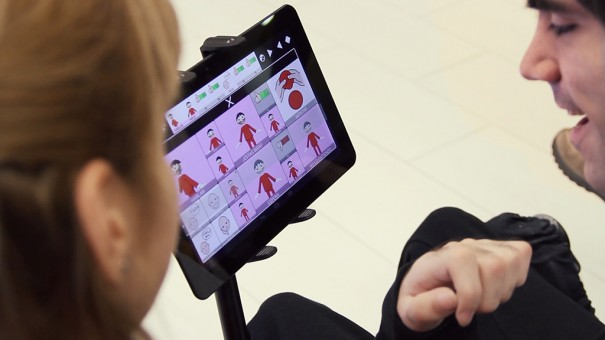
\includegraphics[width=0.7\textwidth,height=\textheight]{media/articulo05_image2.jpeg}}

\End{centerimageenv}

\Begin{smalltextenv}

\textbf{Imagen 1:} Persona usando Accessibility Scan \textbf{Fuente:} \href{https://www.digitalavmagazine.com/2015/03/25/accessibility-scan-facilita-la-interaccion-con-terminales-android-a-personas-con-movilidad-reducida/}{\emph{Digital AV magazine}}

\End{smalltextenv}

\Begin{multicols}{2}

\begin{itemize}
\item
  \emph{Suite,} Accesibilidad Android que es una colección de aplicaciones que permiten usar el dispositivo sin usar la vista o con un dispositivo conmutador.
\item
  \emph{Voice Access,} permite utilizar el dispositivo por medio de la voz, muy útil para personas con discapacidades físicas.
\item
  \emph{Talkback,} proporciona comentarios en voz alta de lo que se está mostrando en la pantalla para ayudar a las personas con problemas de visión a utilizar el dispositivo.
\item
  \emph{Taptapsee,} permite a las personas no videntes tomar una fotografía de un objeto y escuchar una descripción de él.
\item
  \emph{Dilo en señas,} aplicación para practicar el lenguaje de señas traducido al español.
\item
  \emph{Good Vibes,} es una aplicación diseñada para sordociegos que permite enviar y recibir mensajes en código morse.
\end{itemize}

\hypertarget{articulo05_cross03}{}
\spacefourmilis

Lastimosamente en Guatemala, en el último censo nacional de población y vivienda se dieron a conocer los siguientes datos con respeto a las TIC: se contabilizó que a nivel nacional un 62\% cuenta teléfono celular, 21\% utiliza computadora y 29\% tiene acceso a internet. También que 19\% tiene computadora, celular e internet; 19\% computadora y celular; 20\% computadora e internet y 28\% celular e internet.\protect\hyperlink{articulo05_ref03}{{[}3{]}}

Tomando en cuenta estos porcentajes, se hace evidente que son muy pocos guatemaltecos con discapacidades quienes pueden acceder a estas tecnologías las cuales les serían de gran ayuda para su vida cotidiana y para tener mejores oportunidades en el ámbito laboral.

Por otro lado, existe mucha desinformación sobre las distintas discapacidades que existen y los procedimientos para tratarlas de la mejor manera, así como de formas sencillas que pueden utilizarse para ayudar a estas personas. Muchas veces es difícil la comunicación con personas con diferencias físicas, sensoriales o de algún otro tipo, lo cual no debería existir ya que es trabajo de todos hacer un país inclusivo, equitativo y con cero discriminaciones.

Yendo más allá de las TIC, existen aplicaciones que funcionan junto con el internet de las personas \emph{loP} para brindar una mejor ayuda.

Una muestra de esto es OttoBock, una empresa alemana que se dedica a la fabricación de prótesis, la cual está introduciendo inteligencia artificial con \emph{IoP} en sus productos, para que estos aprendan de las personas que los usan.

La forma en que los productos interactúan con \emph{IoP} se basa en el análisis de los datos, ya que la prótesis recibe señales que debe aprender y con base en ellas realizar un determinado movimiento y con esto sucesivamente reconocer más movimientos.

\spacefourmilis

\emph{Myo plus} es un producto lanzado en mayo del 2019, el cual es una mano protésica multiarticulada con inteligencia artificial que permite reconocer las señales que envía el cerebro para realizar la acción sin necesidad de requerir gran concentración por parte de la persona que lo usa mientras que el dispositivo va aprendiendo los distintos movimientos para tenerlos disponibles con más facilidad. Además, cuenta con una aplicación móvil que permite ver los patrones de movimiento que recibe la prótesis, para así afinar los movimientos y hacerlos más precisos según sea la necesidad, tomando en cuenta que puede calibrarse cada vez que lo desea. (imagen \#2)

Es compatible con otros dispositivos de la misma empresa, lo cual permite ajustarlo con facilidad a otras terminales para tener mejor control.

Esta es tan solo una de las prótesis existentes que utilizan esta tecnología la cual ayuda en gran manera a las personas para desarrollarse con naturalidad e independencia, pero existen muchas más que pudieran estar al alcance de mayor cantidad de personas.

De igual forma muchas de estas soluciones no son conocidas por personas que pudieran tener acceso a ellas, dentro de los programas de ayuda debería darse a conocer la mayor cantidad de tecnologías para que todas las personas puedan tener una vida digna.

\End{multicols}

\spacefourmilis

\Begin{centerimageenv}

\href{https://www.ottobock.es/protesica/miembro-superior/sistemas-de-brazo-y-mano/myo-plus/index.html}{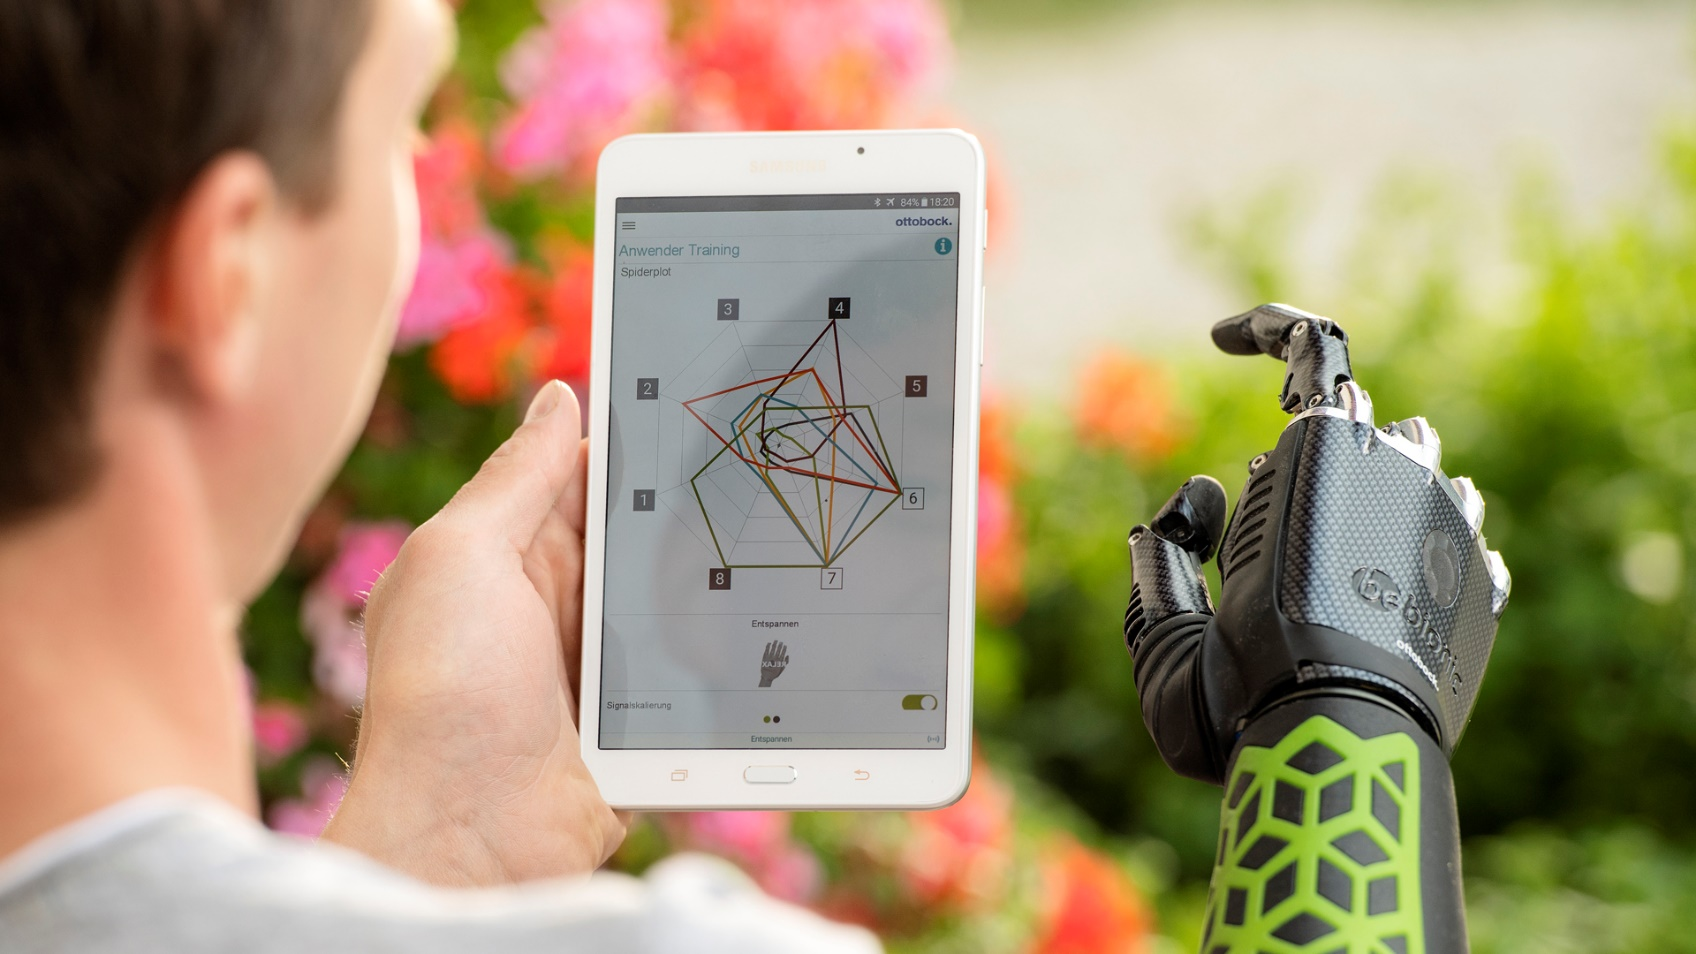
\includegraphics[width=1\textwidth,height=\textheight]{media/articulo05_image3.jpeg}}

\End{centerimageenv}

\Begin{smalltextenv}

\textbf{Imagen 2:} Prótesis Myo Plus \textbf{Fuente:} \href{https://www.ottobock.es/protesica/miembro-superior/sistemas-de-brazo-y-manhttps://www.youtube.com/watch?time_continue=36\&v=DdZVbCHhMVU\&feature=emb_logo}{Ottobock}

\End{smalltextenv}

\Begin{multicols}{2}

\hypertarget{conclusiones-4}{%
\section*{Conclusiones}\label{conclusiones-4}}
\addcontentsline{toc}{section}{Conclusiones}

\begin{itemize}
\tightlist
\item
  \emph{IoP} es el análisis de los datos de todas las identidades digitales de las personas, esto para poder conocerlas mejor y brindarles soluciones adaptadas a sus necesidades.
  \spacefivemilis
\item
  Las TIC buscan hacer más fácil y accesible la educación para todas las personas.
  \spacefivemilis
\item
  La CONAID cuenta con programas para la integración de personas con discapacidad, para que tengan acceso a recursos tecnológicos que los ayuden a llevar una vida más cómoda.
  \spacefivemilis
\item
  Muchas de las aplicaciones existentes de ayuda a personas con discapacidades, no son conocidas, por lo que deberían tener más publicidad de manera que la mayor cantidad de personas pueda ayudarse con ellas.
  \spacesixmilis
\item
  \emph{Myo Plus} es una prótesis muy avanzada en tecnología que es de gran ayuda para las personas con amputaciones de brazo, hace que las personas puedan realizar las tareas diarias con menos dificultad.
\end{itemize}

\hypertarget{referencias-4}{%
\section*{Referencias}\label{referencias-4}}
\addcontentsline{toc}{section}{Referencias}

\begin{itemize}
\item
  \hypertarget{articulo05_ref01}{}

  \protect\hyperlink{articulo05_cross01}{{[}1{]}} \href{http://conadi.gob.gt/}{«Conadi»}, \href{http://conadi.gob.gt/web/2017/03/21/presentacion-de-resultados-de-la-encuesta-nacional-de-discapacidad/}{Presentación De Resultados De La Encuesta Nacional De Discapacidad}, 21 marzo 2017. {[}En línea{]}. Disponible en: \url{https://bit.ly/2ZEpCIK}. {[}Último acceso: 05 marzo 2020{]}.
  \spaceminusmilis
\item
  \hypertarget{articulo05_ref02}{}

  \protect\hyperlink{articulo05_cross02}{{[}2{]}} \href{https://bibliosabana.wordpress.com/}{«Biblioteca Octavio Arizmendi Posada»}, \href{https://bibliosabana.wordpress.com/2014/06/13/tecnologias-para-el-acceso-a-la-informacion-de-personas-con-discapacidad-visual/}{Tecnologías para el acceso a la información de personas con discapacidad visual}, 13 junio 2014. {[}En línea{]}. Disponible en: \url{https://bit.ly/3fHJ2Cl}. {[}Último acceso: 11 marzo 2020{]}.
  \spaceminusmilis
\item
  \hypertarget{articulo05_ref03}{}

  \protect\hyperlink{articulo05_cross03}{{[}3{]}} \href{https://elperiodico.com.gt/}{«El Periodico»}, \href{https://elperiodico.com.gt/inversion/2019/10/08/censo-refleja-brechas-en-el-uso-de-internet/}{Censo refleja brechas en el uso de Internet}, 08 octubre 2019. {[}En línea{]}. Disponible en: \url{https://bit.ly/2OADmOs}. {[}Último acceso: 29 febrero 2020{]}.
  \spaceminusmilis
\item
  \hypertarget{articulo05_ref04}{}

  {[}4{]} \href{http://polidoc.usac.edu.gt}{«Dayan Roselyn De León Cermeño»}, \href{http://polidoc.usac.edu.gt/digital/cedec11272.pdf}{Análisis del uso de tecnologías de la información y comunicación}, 30 noviembre 2017. {[}En línea{]}. Disponible en: \url{https://bit.ly/3eGFpv6}. {[}Último acceso: 26 febrero 2020{]}.
  \spaceminusmilis
\item
  \hypertarget{articulo05_ref05}{}

  {[}5{]} \href{https://aspace.org/}{«ISDE TICs»}, \href{https://aspace.org/blog/705/control-de-entorno}{Análisis sectorial enfocado en oportunidades}, 30 agosto 2016. {[}En línea{]}. Disponible en: \url{https://bit.ly/2ZI2l8Z}. {[}Último acceso: 28 febrero 2020{]}.
\end{itemize}

\End{multicols}

\Begin{centerimageenv}

\href{https://www.facebook.com/UsacFarmaciaUniversitaria/photos/a.425435787516738/2020101148050186/}{
\includegraphics[width=1\textwidth,height=\textheight]{media/articulo05_image5.jpg}}

\End{centerimageenv}

\titleformat{\chapter}[block]{\formatchapterEdDQ}{\labelchapterEdDQ}{\sepchapterEdDQ}{\beforecodechapterEdDQ#1\beforecodechapterparttwoEdDQ}

\titlespacing*{\chapter} {\leftchapterEdDQ}{\beforesepchapterEdDQ}{\afterchapterEdDQ}

\titleformat{\section}[block]{\formatsection}{\labelsection}{\sepsection}{\beforecodesection#1}

\titleformat{\subsection}[block]{\formatsubsection}{\labelsubsection}{\sepsubsection}{\beforecodesubsection#1}

\titleformat{\subsubsection}[block]{\formatsubsubsection}{\labelsubsubsection}{\sepsubsubsection}{\beforecodesubsubsection#1}

\hypertarget{article06}{%
\chapter{Nuclear vs.~Renovable}\label{article06}}

\BeginKnitrBlock{photobiography3}{media/articulo06_image1.png}
\begin{styleAuthorName}

Mario Jeancarlo Morales Rivas

\end{styleAuthorName}

\begin{styleAuthormail}

\href{mailto:jeancarlo64091@gmail.com}{\nolinkurl{jeancarlo64091@gmail.com}}

\end{styleAuthormail}

Estudiante de Ingeniería en Ciencias y Sistemas - USAC

\begin{styleKeywords}

\textbf{Palabras Clave:}\\
Nuclear, renovable, Cambio climático, desechos energéticos, planes energéticos, medio ambiente.

\end{styleKeywords}
\EndKnitrBlock{photobiography3}

\Begin{multicols}{2}

\hypertarget{introduciendo-nuclear-vs.renovables}{%
\section{Introduciendo Nuclear vs.~Renovables}\label{introduciendo-nuclear-vs.renovables}}

El protagonista caminando solo hacia su destino por un desierto carente de vida es la típica escena con la que inician las películas postapocalípticas de la época, planteando un futuro vacío y duro para el ser humano. Es triste pensar que un día se llegará a tal desenlace, pero ¿Qué tan lejos está ese futuro? ¿Qué asegura que la humanidad está el camino correcto para evitarlo? ¿Qué se puede hacer para evitar ese destino desolador? Estas son algunas preguntas para evaluar qué tan bien se ha actuado en los últimos años e inferir nuevos rumbos de acción.

Los recursos para la producción de energía son generalmente de naturaleza finita por lo cual urge maximizar su utilización. Y es que mientras la población humana crece exponencialmente, los recursos escasean cada día más. Miles mueren de hambre al día, familias viven en la pobreza y muchos otros se encuentran aislados. Puede considerarse al planeta Tierra como un conjunto de recursos en sí mismo, pero estos recursos no son ilimitados. Es más, actualmente existe un enorme problema en el medio ambiente: El cambio climático. Un elemento que impacta sobremanera en el cambio climático es la generación de energía pues de su fuente depende el aumento de la temperatura mundial.

En un mundo tecnológico, un recurso vital para el desarrollo humano es la energía eléctrica. Un bien que todos luchan por producir y hacer accesible para todos. Cada país posee su propio plan energético mediante el cual buscan optimizar las fuentes de energía para impulsar el desarrollo de su población. Así, las energías renovables surgen como una forma de producir energía limpia de manera sustentable. En la actualidad las energías renovables son consideradas la mejor fuente energética, pero ¿es la energía renovable la mejor fuente energética o existen opciones más viables? Mediante este artículo se pretende realizar una exposición sobre cual fuente energética es mejor e impacta menos el medio ambiente.

\spacefivemilis

\hypertarget{conceptos-previos}{%
\section{Conceptos previos}\label{conceptos-previos}}

\spaceminusmilis

\begin{enumerate}
\def\labelenumi{\arabic{enumi}.}
\item
  {Energías renovables:} Son fuentes de energía basadas en el uso de recursos de origen natural renovables. Por ejemplo, la biomasa vegetal, el viento, el sol o el agua. Al utilizar recursos naturales renovables se logra crear energía de manera ilimitada sin perjudicar de manera directa al medio ambiente.
\item
  {Panel solar:} Es un dispositivo que recibe energía solar para luego producir energía eléctrica o calor. Pueden dividirse los paneles solares en colectores y fotovoltaicos. Los primeros son utilizados para producir agua caliente en su mayoría para uso doméstico. Mientras que los fotovoltaicos están compuestos de muchas celdas que absorben los rayos solares para generar electricidad. A lo largo de este artículo el uso de panel solar alude exclusivamente a paneles solares fotovoltaicos.
\item
  {Turbina eólica:} Es un aparato mecánico que convierte la energía del viento en energía eléctrica. Inicialmente percibe la energía proveniente del viento convirtiéndola en energía mecánica la cual se almacena en baterías. Las turbinas deben estar a grandes alturas para optimizar el aire percibido.
\item
  {Energía nuclear:} Es el tipo de energía contenida dentro del núcleo de un átomo. Esta energía puede ser liberada a través de fisión o fusión nuclear. En la fusión nuclear los átomos se juntan para crear energía, mientras que en la fisión los núcleos se separan creando núcleos más pequeños y energía.
\item
  {Reactor nuclear:} Es una instalación que tiene la capacidad de iniciar, mantener y controlar reacciones de fisión nuclear en cadena. Un reactor nuclear puede tener un diseño térmico o rápido.
\item
  {Cambio climático:} El cambio climático no es un concepto nuevo, ya que en el pasado ya ha habido importantes cambios climáticos, por ejemplo, el último periodo glaciar. Sin embargo, en la actualidad se ha presentado un repunte histórico en la temperatura, esto debido a las emisiones de gases. Gases denominados gases de efecto invernadero, ya que incrementan la capacidad atmosférica de retener calor, dando lugar al calentamiento global.
\end{enumerate}

\hypertarget{impacto-de-granjas-euxf3licas-y-solares-en-el-medio-ambiente}{%
\section{Impacto de granjas eólicas y solares en el medio ambiente}\label{impacto-de-granjas-euxf3licas-y-solares-en-el-medio-ambiente}}

En la actualidad la energía producida por paneles solares y turbinas eólicas es vista como la salvación del mundo, y el único medio con el cual se puede detener el calentamiento global. Se dará inicio al tema abordando lo relativo a las granjas eólicas. Una granja eólica es un conjunto de turbinas eólicas en un área determinada que generan energía eléctrica utilizada para ser distribuida en la zona. Estas granjas no están exentas de problemas, pues las turbinas representan un obstáculo artificial para especies migratorias que atraviesan el espacio aéreo.

\hypertarget{articulo06_cross01}{}
\spacesevenmilis

Michael Shellenberger expone en un artículo de Forbes ``En 2017 un grupo de científicos alertó que el murciélago gris, una especie migratoria podría estar en peligro de extinción si la expansión de las granjas eólicas continua.'' \protect\hyperlink{articulo06_ref01}{{[}1{]}}. Y declara unos párrafos después: ``Las turbinas eólicas amenazan águilas reales, águilas calvas, lechuzas madrigueras, halcones de cola roja, entre muchos otros''. Las granjas solares por su parte demandan un amplio terreno para obtener la cantidad suficiente de rayos solares. Por ello la mayoría de estas granjas son instaladas en desiertos, pero contrario a lo que se pueda pensar los desiertos son hábitats de una rica fauna.

\End{multicols}

\Begin{centerimageenv}

\href{http://savetheeaglesinternational.org/wp-content/uploads/2011/02/pic12-300x200.jpg}{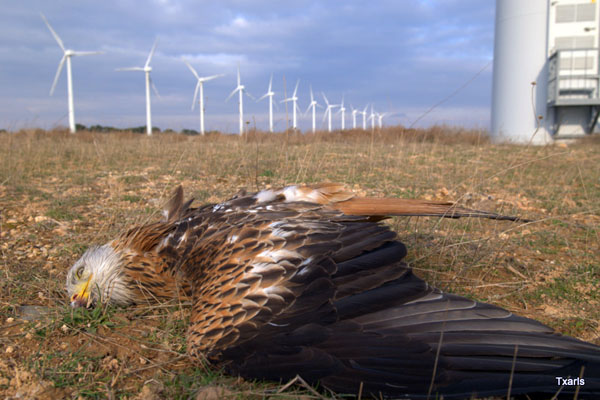
\includegraphics[width=0.75\textwidth,height=\textheight]{media/articulo06_image2.jpeg}}

\End{centerimageenv}

\Begin{smalltextenv}

\textbf{Imagen 1:} Águila agonizando debajo de una turbina \textbf{Fuente:} \href{http://savetheeaglesinternational.org/}{\emph{Association of ecologists GURELUR, Navarre}}

\End{smalltextenv}

\Begin{multicols}{2}

\hypertarget{articulo06_cross02}{}

La cuestión es que las especies no pueden coexistir con las granjas así que son expulsadas. Aunque se ha tratado reubicarlos en reservas naturales, miles de estos animales mueren en este proceso.

Este escenario es retratado en el artículo del periódico ``Los Angeles Times'' escrito por Julie Cart. En este artículo expone lo que ocurrió cuando se creó la granja solar de Ivanpah Valley, California. Cito: ``BrightSource ha gastado \$ 56 millones hasta el momento para proteger y reubicar a las tortugas, pero incluso a ese precio, el trabajo se ha encontrado con una calamidad imprevista: animales aplastados bajo los neumáticos de los vehículos, hormigas guerreras atacando crías en una guardería improvisada y una pequeña tortuga llevada a un nido de águila, su microchip incrustado sonando ligeramente a medida que perecía.'' \protect\hyperlink{articulo06_ref02}{{[}2{]}}

Estos ejemplos evidencian que las energías renovables enfrentan obstáculos naturales, ya que las especies no están acostumbradas o no pueden coexistir con las turbinas ni los paneles solares. Con esto no desea satanizarse a las energías renovables, sino aclarar que incluso las turbinas y paneles presentan inconvenientes que deben ser puestos en una balanza para determinar qué tan beneficioso resulta su uso para el mundo.

\hypertarget{aspectos-negativos-de-las-energuxedas-renovables}{%
\section{Aspectos negativos de las energías renovables}\label{aspectos-negativos-de-las-energuxedas-renovables}}

\hypertarget{articulo06_cross03}{}
\spacesixmilis

Adicionalmente existen aspectos no tan positivos de la energía renovable. La energía solar y eólica es muy difusa, así que se requiere una mayor extensión de terreno para percibir energía por lo cual deben realizarse inversiones significativas en extensiones de tierra para obtener energía eléctrica en las granjas. Como expone el artículo de la Universidad de Leiden ``La energía solar y eólica necesita alrededor de 40-50 veces más espacio que el carbón y 90-100 veces más espacio que el gas.'' \protect\hyperlink{articulo06_ref03}{{[}3{]}}. Es importante reconocer que la tierra será un bien vital para saciar el hambre mundial en los años venideros.

\hypertarget{articulo06_cross04}{}

Otro aspecto a considerar es la deposición de paneles solares al fin de su vida útil ya que no son eternos. De hecho, poseen una vida útil estándar de 25 años en promedio. El problema es que no existe un plan para manejar los residuos generados por los paneles solares. Como Nate expone en su artículo en GreenBiz: ``Parte del problema es que los paneles solares son complicados de reciclar. Están hechos de muchos materiales, algunos peligrosos, y se ensamblan con adhesivos y selladores que dificultan su separación.'' \protect\hyperlink{articulo06_ref04}{{[}4{]}}

\End{multicols}

\spacefourmilis

\Begin{centerimageenv}

\href{https://thumbor.forbes.com/thumbor/960x0/https\%3A\%2F\%2Fblogs-images.forbes.com\%2Fmichaelshellenberger\%2Ffiles\%2F2018\%2F05\%2Fpuerto_rico_solar.jpg}{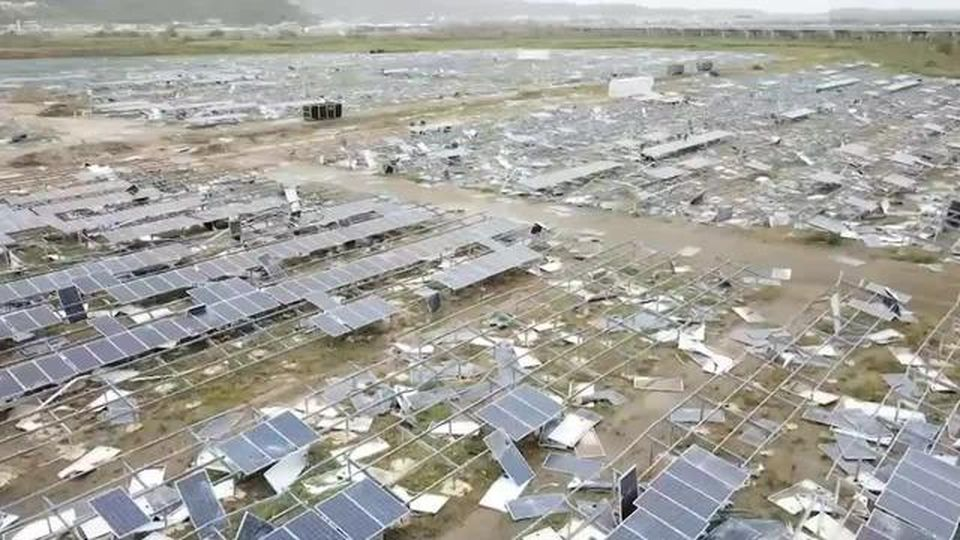
\includegraphics[width=0.75\textwidth,height=\textheight]{media/articulo06_image3.jpeg}}

\End{centerimageenv}

\Begin{smalltextenv}

\textbf{Imagen 2:} Granja solar destruida en Puerto Rico \textbf{Fuente:} \href{https://www.forbes.com/}{Forbes}

\End{smalltextenv}

\Begin{multicols}{2}

\hypertarget{avances-en-energuxeda-nuclear}{%
\section{Avances en energía nuclear}\label{avances-en-energuxeda-nuclear}}

Como se señaló al inicio de este artículo, con la energía nuclear ha ocurrido lo contrario a las energías renovables. La energía nuclear ha sido considerada como la peor fuente de energía, después de los recursos fósiles. Esto debido a un pasado difícil. Hechos puntuales que mancharon la reputación de la energía nuclear hasta nuestros días son: el accidente en la planta nuclear de Chernobyl en 1986, siendo este el peor accidente nuclear hasta la fecha y las dos bombas nucleares detonadas en la segunda guerra mundial.

Sin embargo, la energía nuclear ha avanzado mucho en los últimos años. De hecho, la energía nuclear es una de las fuentes energéticas más seguras de nuestros días. Como puede apreciarse en la imagen \#3 extraída de Our World in Data, solo el 0.01\% de las muertes suscitadas por la producción energética es nuclear. Otro punto a notar es que la energía nuclear es superada por la energía eólica y solar en este gráfico con 0.035\% y 0.019\% respectivamente.

\Begin{centerimageenv}

\href{https://ourworldindata.org/safest-sources-of-energy}{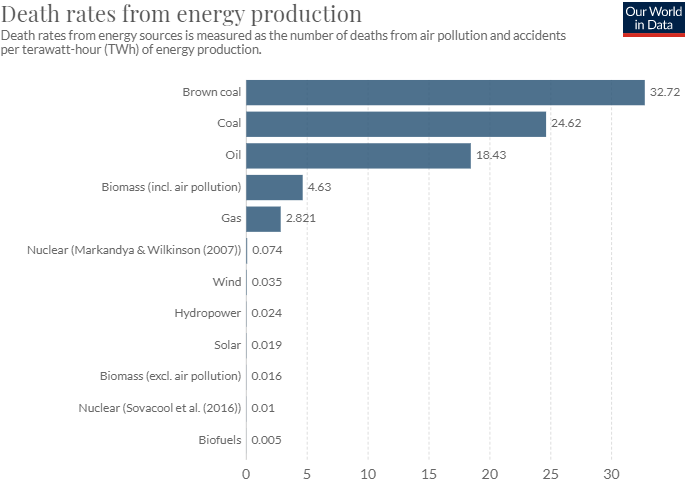
\includegraphics[width=0.5\textwidth,height=\textheight]{media/articulo06_image4.png}}

\End{centerimageenv}

\Begin{smalltextenv}

\textbf{Imagen 3:} Indice de muertes en producción energética \textbf{Fuente:} \href{https://ourworldindata.org/safest-sources-of-energy/}{Markandya and Wilkinson}

\End{smalltextenv}

\spacefourmilis

Para finalizar la sección sobre energía nuclear a continuación se presentan otros aspectos positivos de ésta, en los cuales se considera supera a las energías renovables. Los isótopos nucleares, que son los combustibles de las plantas nucleares no requieren mucho espacio. Por ende, la extensión de terreno necesario para su producción es menor en comparación con la amplia extensión requerida por las granjas de energía renovable.

Hablando de los residuos, los paneles solares requieren 17 veces más materiales que las plantas nucleares. Por lo tanto, el mantenimiento de los residuos se dificulta más con los paneles. Además, los residuos nucleares son los únicos desechos en producción eléctrica que pueden almacenarse de manera segura, los demás desechos se emiten directamente al medio ambiente

\hypertarget{comparaciuxf3n-del-plan-energuxe9tico-de-alemania-y-francia}{%
\section{Comparación del plan energético de Alemania y Francia}\label{comparaciuxf3n-del-plan-energuxe9tico-de-alemania-y-francia}}

\hypertarget{articulo06_cross05}{}

Aún con estos datos podrían existir dudas sobre cual fuente energética es mejor, pero en 2019 se crearon estadísticas reales de dos programas energéticos que utilizaron distintas fuentes, siendo nucleares y renovables. Alemania inició un programa para convertirse en un país que solo dependería de fuente de energía renovable. Por otro lado, Francia confió en un programa nuclear para obtener la mayor parte de su energía. En la referencia \protect\hyperlink{articulo06_ref05}{{[}5{]}} se puede apreciar la comparación de estos dos programas energéticos.

Es interesante observar que la energía en Francia es 86\% limpia en comparación con Alemania donde la energía es solo 39\% limpia. Además, se puede ver que la energía en Alemania es 70\% más cara que en Francia. La energía en Alemania decayó de sobremanera luego que prescindiera de la energía nuclear.

\hypertarget{conclusiones-5}{%
\section*{Conclusiones}\label{conclusiones-5}}
\addcontentsline{toc}{section}{Conclusiones}

\begin{itemize}
\item
  A pesar de los beneficios que posee el uso de la energía solar y eólica, entre los cuales resalta el uso de fuentes de energía ilimitadas, estas energías renovables generan impactos negativos en el medio ambiente.
\item
  Contrario a las creencias negativas existentes sobre la energía nuclear, actualmente es una de las más seguras y limpias, y con más ventajas que las renovables como por ejemplo: la utilización de terrenos menos extensos y el uso de una cantidad considerablemente menor de materiales requeridos en comparación con los paneles solares.
\item
  La energía nuclear, al ser más fiable, generando energía de manera más estable, tiene un costo menor para la población, lo cual se ha evidenciado en países como Alemania que, por un costo mayor, obtiene sólo la mitad de energía que Francia obtiene de energía nuclear.
\end{itemize}

\hypertarget{referencias-5}{%
\section*{Referencias}\label{referencias-5}}
\addcontentsline{toc}{section}{Referencias}

\begin{itemize}
\item
  \hypertarget{articulo06_ref01}{}

  \protect\hyperlink{articulo06_cross01}{{[}1{]}} \href{http://www.forbes.com/}{«Forbes»}, \href{https://www.forbes.com/sites/michaelshellenberger/2019/06/26/why-wind-turbines-threaten-endangered-species-with-extinction/\#63a07d1264b4}{Why Wind Turbines Threaten Endangered Species With Extinction}, 26 junio 2016. {[}En línea{]}. Disponible en: \url{https://bit.ly/2OGwAH2}. {[}Último acceso: 08 marzo 2020{]}.
\item
  \hypertarget{articulo06_ref02}{}

  \protect\hyperlink{articulo06_cross02}{{[}2{]}} \href{https://www.latimes.com}{«Los Angeles Times»}, \href{https://www.latimes.com/archives/la-xpm-2012-mar-04-la-me-solar-tortoise-20120304-story.html/}{Saving desert tortoises is a costly hurdle for solar projects}, 04 marzo 2012. {[}En línea{]}. Disponible en: \url{https://lat.ms/2CMQDRm}. {[}Último acceso: 01 marzo 2020{]}.
\item
  \hypertarget{articulo06_ref03}{}

  \protect\hyperlink{articulo06_cross03}{{[}3{]}} \href{https://phys.org/}{«Phys.org»}, \href{https://phys.org/news/2018-08-renewable-energy-sources-space-fossil.html}{Renewable energy sources can take up to 1000 times more space than fossil fuels}, 28 agosto 2018. {[}En línea{]}. Disponible en: \url{https://bit.ly/39iB3sT}. {[}Último acceso: 01 marzo 2020{]}.
  \spacetwomilis
\item
  \hypertarget{articulo06_ref04}{}

  \protect\hyperlink{articulo06_cross04}{{[}4{]}} \href{https://www.greenbiz.com/}{«GreenBiz»}, \href{https://www.greenbiz.com/article/what-will-happen-solar-panels-after-their-useful-lives-are-over}{Análisis del uso de tecnologías de la información y comunicación}, 11 mayo 2018. {[}En línea{]}. Disponible en: \url{https://bit.ly/3fLV1P7}. {[}Último acceso: 05 marzo 2020{]}.
  \spacetwomilis
\item
  \hypertarget{articulo06_ref05}{}

  {[}5{]} \href{http://environmentalprogress.org/}{«Environmental progresss»}, \href{http://environmentalprogress.org/germany}{Germany vs.~France energy production in numbers}, 03 septiembre 2019. {[}En línea{]}. Disponible en: \url{https://bit.ly/30qxdKi}. {[}Último acceso: 06 marzo 2020{]}.
\end{itemize}

\End{multicols}

\Begin{centerimageenv}

\href{https://dtt-ecys.org}{
\includegraphics[width=0.25\textwidth,height=\textheight]{media/logo_50.png}}

\End{centerimageenv}

\Begin{centerimageenv}

\href{https://edc.ccqqfar.usac.edu.gt/}{
\includegraphics[width=1\textwidth,height=\textheight]{media/articulo06_image5.png}}

\End{centerimageenv}

\titleformat{\chapter}[block]{\formatchapterEdDQ}{\labelchapterEdDQ}{195pt}{\beforecodechapterEdDQ#1\beforecodechapterparttwoEdDQ}

\titlespacing*{\chapter} {\leftchapterEdDQ}{\beforesepchapterEdDQDobleLine}{\afterchapterEdDQDobleLine}

\titleformat{\section}[block]{\formatsection}{\labelsection}{\sepsection}{\beforecodesection#1}

\titleformat{\subsection}[block]{\formatsubsection}{\labelsubsection}{\sepsubsection}{\beforecodesubsection#1}

\titleformat{\subsubsection}[block]{\formatsubsubsection}{\labelsubsubsection}{\sepsubsubsection}{\beforecodesubsubsection#1}

\hypertarget{article07}{%
\chapter{Agrotecnología: Una opción para la agricultura guatemalteca}\label{article07}}

\BeginKnitrBlock{photobiography3}{media/articulo07_image1.png}
\begin{styleAuthorName}

Bayron Romeo Axpuac Yoc

\end{styleAuthorName}

\begin{styleAuthormail}

\href{mailto:bayronaxpuac95@gmail.com}{\nolinkurl{bayronaxpuac95@gmail.com}}

\end{styleAuthormail}

Estudiante de Ingeniería en Ciencias y Sistemas - USAC

\begin{styleKeywords}

\textbf{Palabras Clave:}\\
Transformación digital, automatización, Guatemala, tecnología.

\end{styleKeywords}
\EndKnitrBlock{photobiography3}

\Begin{multicols}{2}

\hypertarget{articulo07_cross01}{}

La agricultura es una actividad del sector primario de la economía. Mediante ella el hombre realiza la modificación de su entorno ecológico para generar una producción que le permita obtener alimentos para su subsistencia. La agricultura es una de las fuentes más importantes para el desarrollo de Guatemala, debido a que una parte significativa de sus habitantes se dedican a esta actividad para obtener su sustento diario. Se estima que existe más de 1 millón de hogares agrícolas que representan aproximadamente 6.2 millones de personas, quienes cultivan su propia comida y crían sus propios animales. Además, se estima que la actividad agrícola ocupa aproximadamente el 63\% del empleo agropecuario; este genera un 40\% de las exportaciones que realiza el país \protect\hyperlink{articulo07_ref01}{{[}1{]}}.

\Begin{centerimageenv}

\href{https://www.guatemala.com/fotos/2019/07/Agricultura-Familiar-Guatemala-ONU-Economia-0.jpg/}{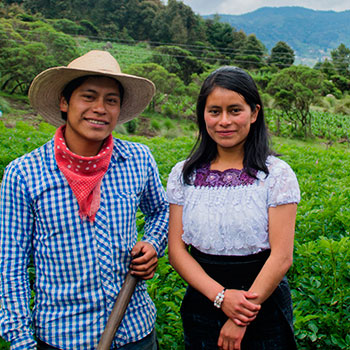
\includegraphics[width=0.45\textwidth,height=\textheight]{media/articulo07_image2.jpeg}}

\End{centerimageenv}

\Begin{smalltextenv}

\textbf{Imagen 1:} Agricultores en Guatemala \textbf{Fuente:} \href{https://www.guatemala.com/}{\emph{Guatemala}}

\End{smalltextenv}

\hypertarget{articulo07_cross02}{}

Guatemala es un país caracterizado por su riqueza natural y cultural, cuya ascendencia e historia le ha conducido al desarrollo de diferentes actividades agrícolas. En Guatemala, el maíz es la mayor superficie cultivada, seguido por las plantaciones de café, la caña de azúcar y el frijol. Juntamente con la ganadería, la caza, silvicultura y la pesca aportan el 14\% del producto interno bruto (PIB) del país \protect\hyperlink{articulo07_ref02}{{[}2{]}}

La agricultura guatemalteca emplea un conjunto de técnicas y herramientas para la producción de alimentos libres de contaminantes con altos estándares de calidad, lo cual se logra mediante el uso de diversos sistemas de cultivo. Estos sistemas son aplicados a explotaciones agrícolas de los recursos básicos (agua, tierra, zonas de pastoreo, bosques, otros) y empresariales, implementando planes de desarrollo agrícola para su mantenimiento. Entre las herramientas y sistemas de cultivo utilizados por los guatemaltecos se encuentran:
\hypertarget{articulo07_cross03}{}

\begin{itemize}
\item
  \textbf{Sistema de cultivo con riego} Este sistema consiste en aplicar agua a cada uno de los cultivos por medio del suelo, cubriendo la necesidad hídrica de las plantaciones, lo que incrementa la producción agrícola al transformar zonas de agricultura de secano en zonas de regadío. Esto permite la producción intensiva de arroz, frutas y hortalizas. Este sistema es más utilizado en Zacapa y El Progreso \protect\hyperlink{articulo07_ref03}{{[}3{]}}
\item
  \textbf{Sistema de cultivo intensivo en montaña o tierras altas}: Este sistema se desarrolla en dos ubicaciones de las montañas o tierras altas. El primero de ellos se lleva a cabo en los valles existentes entre montañas para la producción de hortalizas; la segunda ubicación son las laderas de las montañas. En estas laderas se realiza gran producción de café y hortalizas. Este sistema predomina en el Altiplano Occidental de Guatemala, específicamente en los departamentos de Totonicapán y Quetzaltenango. Estudios Recientes indican que esta técnica fue utilizada en ciudades del período Preclásico y del Clásico de la cultura Maya. Dicho estudio da a conocer que los agricultores de estos periodos realizaban la construcción de terrazas, las cuales se rellenaban con lodo de los bajos (tierra muy fértil); también utilizaban canales de irrigación, cultivo de árboles y abonos; la tala y quema de árboles fueron muy poco utilizadas.
\item
  \textbf{Maquinaria agrícola}. La maquinaria agrícola está conformada por todas aquellas máquinas y equipos que emplean los agricultores en cada una de sus labores. Una máquina agrícola posee una dependencia de funcionamiento y la mayoría de veces depende de un motor de combustión y mecanismos de transmisión permitiendo su desplazamiento por el área de trabajo.
\item
  \textbf{Agrimensura} La agrimensura es la disciplina que permite llevar a cabo mediciones utilizando herramientas como: la brújula, la cinta métrica, el teodolito, niveles, piquetes, entre otros, la ubicación, identificación, delimitación, medición, representación y valuación del espacio y la propiedad territorial.
\end{itemize}

La agricultura es uno de los sectores productivos más importantes y antiguos que posee la sociedad guatemalteca, ya que del desarrollo de esta actividad depende la alimentación de la población. Por lo general en este país se asocia la agricultura con la tradición; métodos antiguos para cultivar, maquinaria manual, procesos ortodoxos para la siembra y cosecha. La agricultura guatemalteca busca satisfacer las necesidades de alimentación de la creciente población, por lo que es un desafío mayor evitar el mal uso de los recursos naturales velando por la salud de la población y reduciendo los costos de producción. Ante este desafío, surge un aliado que avanza firmemente en el mundo: \textbf{la Agrotecnología}. Aunque la agricultura y la tecnología abarcan áreas totalmente distintas, la tecnología aporta herramientas importantes para la producción de frutas, hortalizas y otros tipos de productos agrícolas, además, gracias al uso de la Agrotecnología todo el proceso de generación de alimentos para el cultivo, siembra, cosecha y empaque pueden ser supervisadas por medio de sus herramientas tecnológicas.

\End{multicols}

\spacefourmilis

\Begin{centerimageenv}

\href{https://es.wikipedia.org/wiki/Maquinaria_agr\%C3\%ADcola\#/media/Archivo:Agricultural_machinery.jpg}{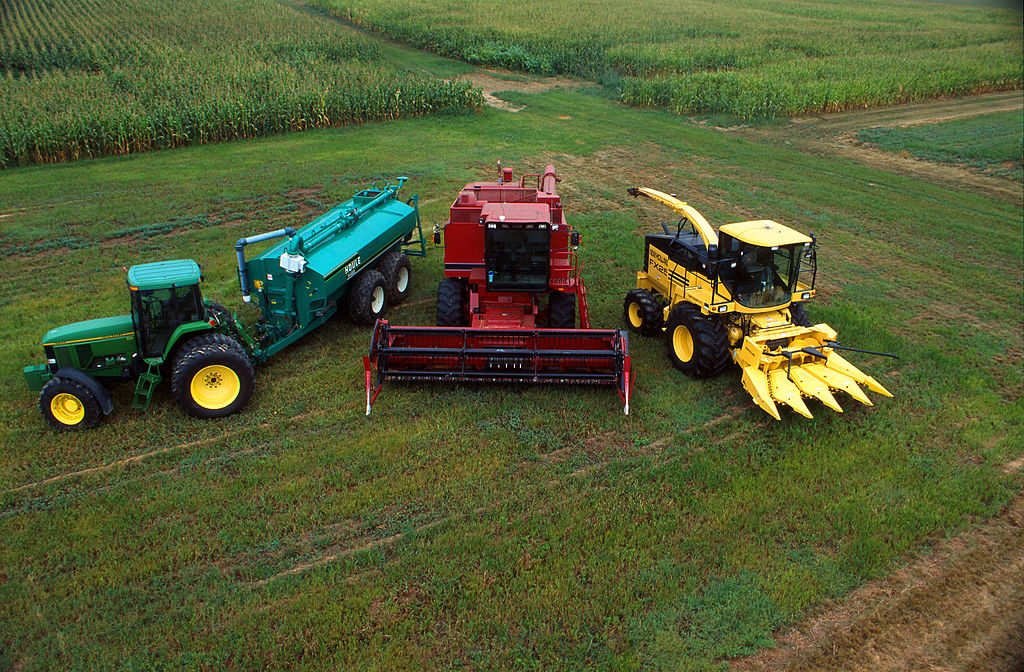
\includegraphics[width=0.82\textwidth,height=\textheight]{media/articulo07_image3.jpeg}}

\End{centerimageenv}

\Begin{smalltextenv}

\textbf{Imagen 2:} Maquinaria Agrícola. \textbf{Fuente:} \href{https://www.wikipedia.com/}{Wikipedia}

\End{smalltextenv}

\Begin{multicols}{2}

La Agrotecnología emplea las herramientas tecnológicas necesarias para una óptima producción dando como resultado en la actualidad una transformación digital en el área agrícola, lo que resulta ser un factor importante en el crecimiento económico, pues interviene en los diversos elementos de la agricultura tales como: la producción de alimentos, la maquinaria, el personal involucrado, los recursos naturales, sistemas de cultivos, con el objetivo de mantener la calidad de vida, promoviendo la cultura económica y los valores.

La transformación digital que se aplica en el área agrícola permite el ingreso de nuevas tecnologías en diversas áreas con el objetivo de optimizar los procesos utilizados, velando por el bienestar del medio ambiente, la producción de alimentos de alta calidad y cubriendo las necesidades alimenticias de la población. Esto sin duda, ayuda lidiar con problemáticas que impactan la agricultura actual como el cambio climático, la malnutrición, la escasez de agua, y el aumento de población.

El sector agrícola guatemalteco tiene un gran campo para beneficiarse de los avances tecnológicos que han sido desarrollados durante los últimos años. La Agrotecnología brinda a la agricultura procesos innovadores y tecnológicos en las actividades del campo, contribuyendo a la reducción del uso de recursos de suma importancia para incrementar la demanda de alimentos. Estas tecnologías pueden aplicarse dentro del sector agrícola guatemalteco de la siguiente forma:

\spacefourmilis

\begin{itemize}
\tightlist
\item
  \textbf{Agroquímica.} Las plantas al igual que los seres humanos sufren de enfermedades y trastornos. Por ejemplo, pueden necesitar de algún nutriente que no pueden producir, sufriendo una insuficiencia que se manifiesta a través de diversos síntomas. Estos síntomas desaparecen cuando se les aporta el nutriente que les faltaba o que tenían en defecto; es acá donde la Agroquímica ocupa espacios en la creación, desarrollo y uso de fertilizantes, nutrientes, plaguicidas y procedimientos fitosanitarios para evitar pérdidas en el área de producción. Gracias a la inteligencia artificial la ciencia de la agroquímica puede examinar los impactos potenciales en la salud así como en el ambiente de cientos de cultivos con precisión milimétrica y de esta forma desarrollar herbicidas, insecticidas, acaricidas, fungicidas y bactericidas.
\end{itemize}

\spacefourmilis

\begin{itemize}
\tightlist
\item
  \textbf{Mecánica y Robótica.} diversos procesos que realizan los agricultores guatemaltecos como el mantenimiento de parcelas, la creación de surcos, manejo y nivelación de tierra, siembra, empaque, distribución de fertilizantes son realizadas por medio de maquinaria controlada por un ser humano, como sembradoras, surcadoras, fumigadoras, tractores, recolectores y en ocasiones estos procesos son realizados manualmente. Gracias a la Agrotecnología estos procesos pueden ser automatizados, utilizando algunas tecnologías como:
  \spaceonemilis

  \begin{itemize}
  \tightlist
  \item
    \textbf{Maquinaria inteligente:} esta tecnología permite al agricultor controlar cualquier máquina por medio de dispositivos móviles, permitiéndole ordenar y programar tareas (siembra, surcos, otros) para que estas máquinas trabajen de manera autónoma, acelerando e incrementado así la producción de alimentos, y permitiéndole reducir costos, recursos y mano de obra.
    \spaceonemilis
  \item
    \textbf{Aeronaves pilotadas remotamente (Drones):} brindan modernas y económicas soluciones en la tarea de obtener imágenes de áreas de acceso complicado y permiten el monitoreo de cultivos de forma remota, además el uso y programación de estas aeronaves juntamente con un Sistema de Posicionamiento Global GPS y otras herramientas permitirán la implementación de la Agrimensura de manera óptima. (Imagen 3).
    \spaceonemilis
  \item
    \textbf{Sensores remotos:} estos sensores permitirán obtener información de un determinado proceso en la agricultura. Estas herramientas permitirán la captura de datos sobre los cultivos, el suelo, la humedad, precipitaciones, plagas, desarrollo de plantas por medio de redes inalámbricas, dicha información podrá ser procesada y así facilitar la toma de decisiones de diversos aspectos.
    \spaceonemilis
  \end{itemize}
\item
  \textbf{Informática}: esta herramienta utiliza plataformas y aplicaciones digitales para llevar a cabo la administración y el monitoreo de diversos procesos de cultivo.
  \spaceonemilis

  \begin{itemize}
  \tightlist
  \item
    \textbf{Software de gestión:} es un sistema informático conformado por varias herrami-
    entas que permiten realizar tareas adminis-
    trativas, simplificando procesos operativos y productivos. Estos programas permiten realizar el monitoreo y proceso de grandes cantidades de información para que el agricultor mejore la toma de decisiones.
    \spaceonemilis
  \item
    \textbf{Software de geolocalización:} un sistema de geolocalización es una solución de la tecnología de la información que determina la ubicación de un objeto en un entorno físico. Este software proporciona a los agricultores mapas actualizados que alertan sobre cualquier modificación de terrenos para poder controlar las hectáreas de campos de sus sembradíos.
    \spacetwomilis
  \item
    \textbf{E-Commerce agroalimentario:} el comercio electrónico agroalimentario consiste en la compra y venta de productos agrícolas a través de medios electrónicos tal como páginas web. Gracias a esta tecnología las cadenas de distribución conectan directamente a los agricultores con el consumidor final.
    \spaceonemilis
  \end{itemize}
\item
  \textbf{Agricultura sostenible:} se le conoce como agricultura sostenible a toda aquella agricultura que satisface las necesidades de la población sin dañar los recursos naturales y no comprometer a las futuras generaciones con el medio ambiente. Uno de los ejemplos en los cuales el uso de la Agrotecnología permite la agricultura sostenible en Guatemala es en los sistemas de riego de los campos; uno de los sistemas más conocido a nivel mundial es el sistema de riego telemático. Este sistema de riego inteligente analiza las condiciones del ambiente, como el suelo, determinando su humedad y temperatura, luego analiza los datos obtenidos y determina la cantidad de agua que las plantaciones de cultivo necesitan para su crecimiento.
\end{itemize}

\End{multicols}

\spacefourmilis

\Begin{centerimageenv}

\href{https://www.asgrow.com.mx/es-mx/tendencias/el-paquete-de-nutricion-de-acuerdo-a-la-meta-de-rendimiento-a-al1111/_jcr_content/main-par/image.img.jpg/1537543126625.jpg}{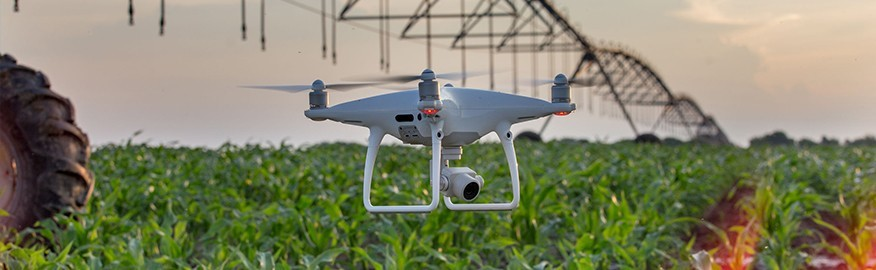
\includegraphics[width=0.9\textwidth,height=\textheight]{media/articulo07_image4.jpg}}

\End{centerimageenv}

\Begin{smalltextenv}

\textbf{Imagen 3:} Drones \textbf{Fuente:} \href{https://www.asgrow.com.mx/}{Asqrow}

\End{smalltextenv}

\Begin{multicols}{2}

\hypertarget{conclusiones-6}{%
\section*{Conclusiones}\label{conclusiones-6}}
\addcontentsline{toc}{section}{Conclusiones}

\begin{itemize}
\item
  El desarrollo tecnológico en la agricultura guatemalteca es de suma importancia, ya que este sector es el encargado de alimentar a la población, por lo tanto la ciencia y la tecnología son elementos importantes para el progreso de la agricultura, pues resulta de gran valor poseer conocimientos sobre las nuevas tecnologías para el cultivo permitiendo así el incremento de la producción agrícola en Guatemala.
\item
  La sociedad actual busca constantemente la optimización en la producción agrícola para solucionar muchos problemas a los que se enfrenta; en dicho sentido la implementación de la Agrotecnología brinda mejoras a los procesos productivos agrícolas, obteniendo mejores y mayores rendimientos, procurando eficacia y eficiencia en el uso de los recursos y ayudando a los agricultores en el desarrollo de sus actividades.
\item
  Para obtener una agricultura sostenible en Guatemala se debe implementar correctamente el uso de las herramientas que nos brinda la Agrotecnología lo cual ayudará a garantizar el buen uso de los recursos naturales que el país posee. Además, la aplicación de la tecnología en el campo agrícola guatemalteco brindará un incremento en la producción y venta de alimentos en los ámbitos nacional e internacional, incrementando el porcentaje de su contribución al producto interno bruto de la nación además de brindar más oportunidades para el desarrollo nacional.
\end{itemize}

\hypertarget{referencias-6}{%
\section*{Referencias}\label{referencias-6}}
\addcontentsline{toc}{section}{Referencias}

\begin{itemize}
\item
  \hypertarget{articulo07_ref01}{}

  \protect\hyperlink{articulo07_cross01}{{[}1{]}} Agricultura \href{https://www.guatemala.com/}{«Guatemala»}, \href{https://www.guatemala.com/desarrollo/economia/agricultura-familiar-tendencia-con-potencial-para-cambiar-guatemala.html}{Agricultura familiar: tendencia con potencial para cambiar Guatemala}, 09 julio 2019. {[}En línea{]}. Disponible en: \url{https://bit.ly/3fKt8H3}. {[}Último acceso: 09 marzo 2020{]}.
\item
  \hypertarget{articulo07_ref02}{}

  \protect\hyperlink{articulo07_cross02}{{[}2{]}} Instituto de Investigación y Proyección sobre Ambiente Natural y Sociedad \href{http://www.infoiarna.org.gt/}{«Infoiarna»}, \href{http://www.infoiarna.org.gt/temas/agricultura/}{Agricultura}, . {[}En línea{]}. Disponible en: \url{https://bit.ly/39iB3sT}. {[}Último acceso: 09 marzo 2020{]}.
\item
  \hypertarget{articulo07_ref03}{}

  \protect\hyperlink{articulo07_cross03}{{[}3{]}} Rubén Elías González \href{https://es.scribd.com/}{«Scribd»}, \href{https://es.scribd.com/document/318239266/SISTEMA-DE-CULTIVOS-DE-GUATEMALA-docx}{Sistema de Cultivos de Guatemala}, 14 julio 2016. {[}En línea{]}. Disponible en: \url{https://bit.ly/3fMfWS9}. {[}Último acceso: 10 marzo 2020{]}.
\end{itemize}

\spaceminusmilis

\begin{itemize}
\item
  \hypertarget{articulo07_ref04}{}

  {[}4{]} Food and Agriculture Organization of the United Nations \href{http://www.fao.org/}{«FAO»}, \href{http://www.fao.org/3/Y1860s/y1860s09.htm}{Principales sistemas de producción agropecuaria en América Latina y El Caribe}, . {[}En línea{]}. Disponible en: \url{https://bit.ly/2ZKEhlC}. {[}Último acceso: 09 marzo 2020{]}.
\item
  \hypertarget{articulo07_ref05}{}

  {[}5{]} \href{http://agricoludec.blogspot.com/}{«AGRICOLUDEC»}, {[}Maquinaria y equipos agrícolas{]} (\url{http://agricoludec.blogspot.com/p/maquinaria-y-equipos-agricola.html}), 02 abril 2017. {[}En línea{]}. Disponible en: \url{https://bit.ly/39d1DDG}. {[}Último acceso: 10 marzo 2020{]}.
\item
  \hypertarget{articulo07_ref06}{}

  {[}6{]} Alejandra González \href{https://news.microsoft.com/}{«News Center LATAM»}, \href{https://news.microsoft.com/es-xl/la-tecnologia-hace-que-la-produccion-agricola-sea-una-actividad-primaria-de-avanzada}{La tecnología hace que la producción agrícola sea una actividad primaria de avanzada}, 31 abril 2015. {[}En línea{]}. Disponible en: \url{https://bit.ly/3eLPrec}. {[}Último acceso: 10 marzo 2020{]}.
\item
  \hypertarget{articulo07_ref07}{}

  {[}7{]} \href{https://agriculturers.com/}{«AGRICULTURERS»}, \href{https://agriculturers.com/agrotecnologia-el-futuro-digital-de-la-agricultura/}{Agrotecnología: el futuro digital de la Agricultura}, 27 marzo 2019. {[}En línea{]}. Disponible en: \url{https://bit.ly/3jiTlih}. {[}Último acceso: 10 marzo 2020{]}.
\item
  \hypertarget{articulo07_ref08}{}

  {[}8{]} Jorge Cartagena \href{https://blogthinkbig.com/}{«Blogthinkbig»}, \href{https://blogthinkbig.com/la-agrotecnologia-una-apuesta-segura-para-las-startups/}{La Agrotecno-
  logía, una apuesta segura para las startups}, 07 noviembre 2011. {[}En línea{]}. Disponible en: \url{https://bit.ly/3fMDMND}. {[}Último acceso: 10 marzo 2020{]}.
\item
  \hypertarget{articulo07_ref09}{}

  {[}9{]} Crédito Real México \href{https://www.creditoreal.com.mx/}{«Crédito Real»}, \href{https://www.creditoreal.com.mx/blog-credito/tecnologia-agricola-para-un-campo-mas-productivo/}{Tecnología agrícola para un campo más productivo}, 10 octubre 2019. {[}En línea{]}. Disponible en: \url{https://bit.ly/32BbcuM}. {[}Último acceso: 10 marzo 2020{]}.
\end{itemize}

\End{multicols}

\Begin{centerimageenv}

\href{http://uviger.fausac.gt/?page_id=235}{
\includegraphics[width=0.55\textwidth,height=\textheight]{media/articulo07_image5.png}}

\End{centerimageenv}

\titleformat{\chapter}[block]{\formatchapterEdDQ}{\labelchapterEdDQ}{\sepchapterEdDQ}{\beforecodechapterEdDQ#1\beforecodechapterparttwoEdDQ}

\titlespacing*{\chapter} {\leftchapterEdDQ}{\beforesepchapterEdDQ}{\afterchapterEdDQ}

\titleformat{\section}[block]{\formatsection}{\labelsection}{\sepsection}{\beforecodesection#1}

\titleformat{\subsection}[block]{\formatsubsection}{\labelsubsection}{\sepsubsection}{\beforecodesubsection#1}

\titleformat{\subsubsection}[block]{\formatsubsubsection}{\labelsubsubsection}{\sepsubsubsection}{\beforecodesubsubsection#1}

\hypertarget{article08}{%
\chapter{Alta disponibilidad con servicios en la Nube}\label{article08}}

\BeginKnitrBlock{photobiography3}{media/articulo08_image1.png}
\begin{styleAuthorName}

José Javier Barreda Mancilla

\end{styleAuthorName}

\begin{styleAuthormail}

\href{mailto:javier.barreda94@gmail.com}{\nolinkurl{javier.barreda94@gmail.com}}

\end{styleAuthormail}

Estudiante de Ingeniería en Ciencias y Sistemas - USAC

\begin{styleKeywords}

\textbf{Palabras Clave:}\\
Redundancia, Fallas, Balanceo de Carga, Principios, DevOps.

\end{styleKeywords}
\EndKnitrBlock{photobiography3}

\Begin{multicols}{2}

La alta disponibilidad es una propiedad que hasta hace algunos años era muy difícil lograr, ya que para que un sistema informático sea altamente disponible existen dos métricas que deben optimizarse:

\begin{itemize}
\item
  El tiempo medio para recuperarse.
  \hypertarget{articulo08_cross01}{}
\item
  El tiempo medio entre cada falla. \protect\hyperlink{articulo08_ref01}{{[}1{]}}
\end{itemize}

Es decir, cuando se habla de un sistema altamente disponible se refiere a un sistema que falla muy pocas veces y cuando lo hace, se recupera en un tiempo muy corto. Esto se logra creando una redundancia de cada una de las partes del sistema, lo que significa que si antes se tenía una fuente de electricidad, ahora son necesarias dos, si se tenía un proveedor de internet, ahora se deben duplicar y así sucesivamente con cada una de las partes del sistema, esto con el fin de que si una falla, se active un proceso que inmediatamente permita que el sistema siga trabajando. Entre más transparente sea este proceso para los usuarios, mayor será la disponibilidad del sistema. Una intervención humana en los procesos de recuperación haría que fuera demasiado lento, por lo que el proceso debe ser totalmente automatizado, solo así se obtendrá un sistema que tiene una baja tasa de fallos y un tiempo de recuperación muy breve.

\spacetwomilis

Si bien la alta disponibilidad es una propiedad muy conveniente, no siempre es necesaria, en aplicaciones que tienen una cantidad limitada de usuarios o que funcionan bajo un horario estricto de trabajo, la alta disponibilidad representa un gasto innecesario, por otra parte, existen aplicaciones como los sitios de comercio electrónico, redes sociales, comunicación o transporte las cuales necesitan que sean accesibles en cualquier momento; para esta clase de aplicaciones la alta disponibilidad es un factor determinante.

\hypertarget{los-servicios-en-la-nube}{%
\section{Los servicios en la nube}\label{los-servicios-en-la-nube}}

\spacetwomilis

Los servicios de la nube permiten que, al momento de crear una aplicación, no sean preocupación varios factores, principalmente el hardware. Para este pueden configurarse las especificaciones que parezcan más convenientes, sin embargo ¿pueden fallar? la respuesta es sí, ¿se recuperan automáticamente? No necesariamente, por esta razón no deben confundirse los términos, un sistema alojado en la nube no necesariamente es de alta disponibilidad.

\spacetwomilis

La nube provee una gama muy amplia de herramientas que se pueden utilizar para este fin, se pueden crear infraestructuras que permitan la rápida recuperación del sistema. Los conceptos no cambian, se crea una redundancia para los dispositivos, se deben monitorear las partes y se crea un proceso de recuperación.

\spacetwomilis

Una de las formas básicas de crear un sistema de alta disponibilidad en la nube es siguiendo la infraestructura de la Imagen \#1.

\Begin{centerimageenv}

\href{https://sites.nubity.com/nubity-blog/wp-content/uploads/sites/4/2018/09/Single-LB.png/}{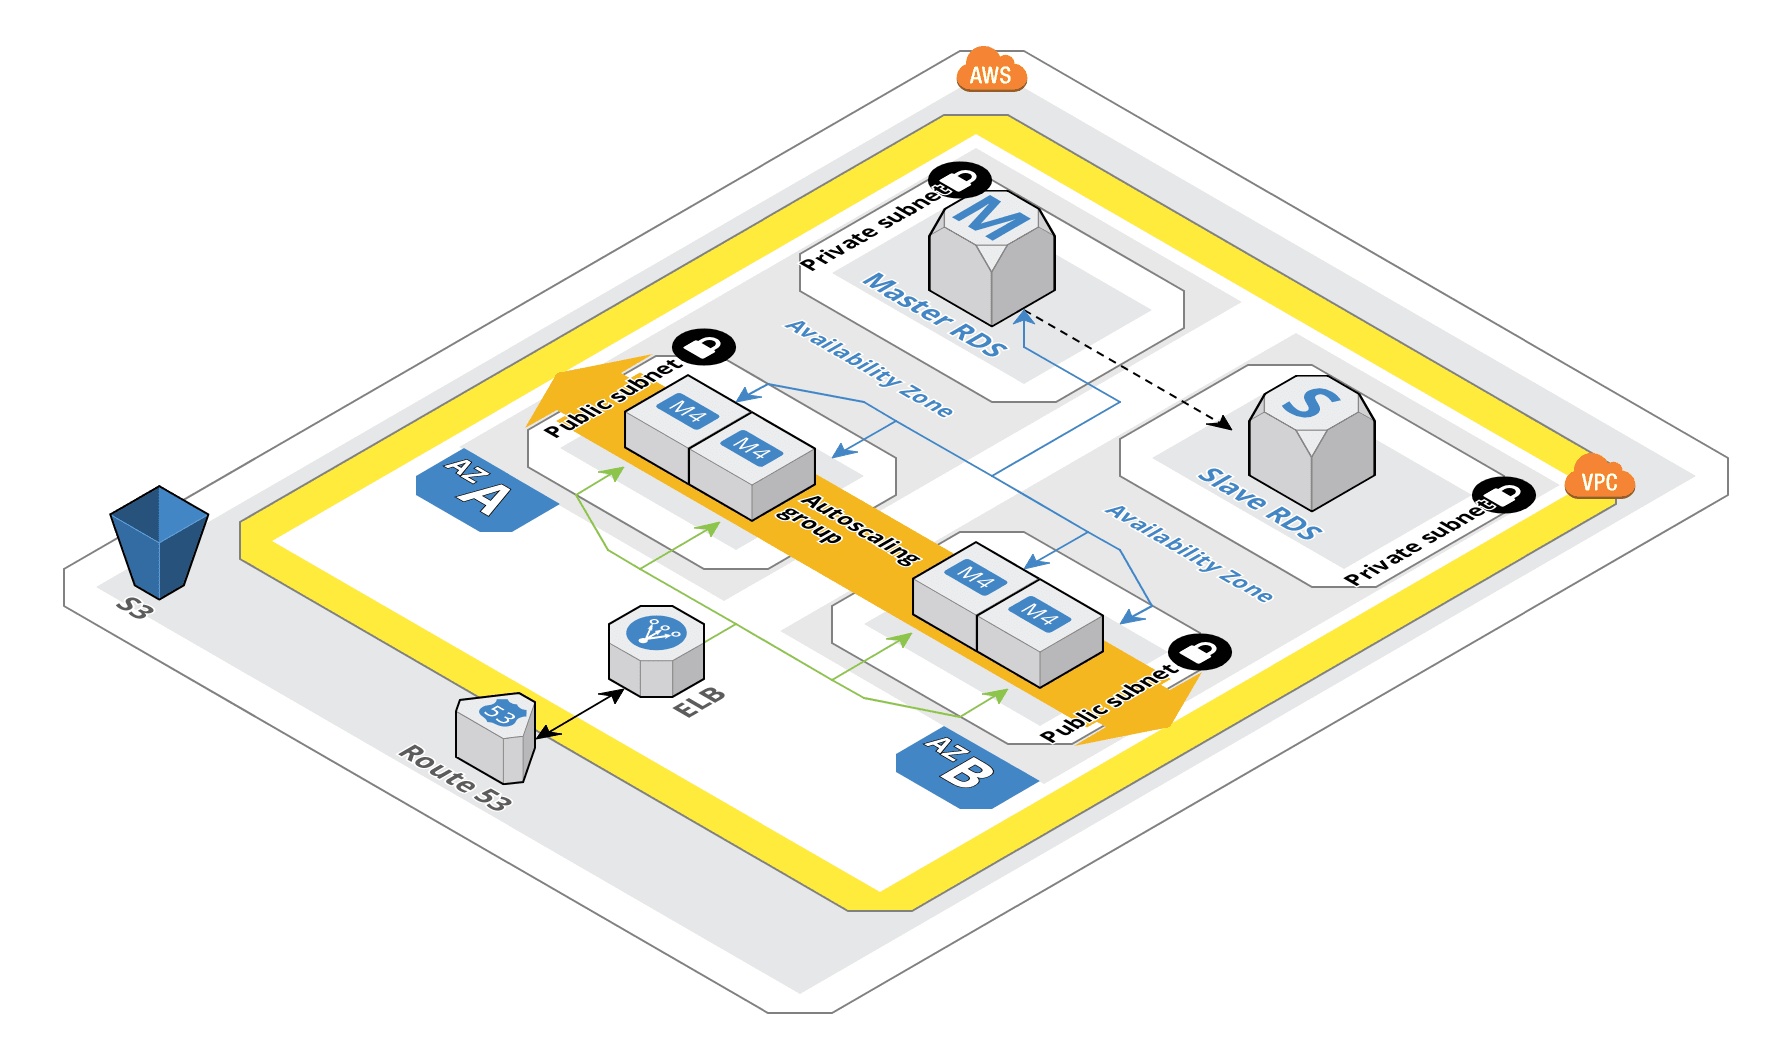
\includegraphics[width=0.48\textwidth,height=\textheight]{media/articulo08_image2.png}}

\End{centerimageenv}

\Begin{smalltextenv}

\textbf{Imagen 1:} Diagrama de Infraestructura de alta disponibilidad en AWS \textbf{Fuente:} \href{https://sites.nubity.com/}{\emph{Nubity}}

\End{smalltextenv}

Tomando como referencia algunos servicios provistos por Amazon Web Services (AWS), en esta infraestructura se pueden encontrar componentes que seguramente tienen sus equivalentes con otros proveedores como Google Cloud o Microsoft Azure:

\hypertarget{articulo08_cross03}{}
\hypertarget{articulo08_cross04}{}
\hypertarget{articulo08_cross05}{}
\hypertarget{articulo08_cross06}{}
\spacetwomilis

\begin{itemize}
\item
  \emph{Route} 53: es un sistema de nombres de dominio (DNS) escalable y altamente disponible. Permite encontrar la dirección IP a la que pertenece un dominio. \protect\hyperlink{articulo08_ref03}{{[}3{]}}
\item
  ELB: el servicio de Balanceo de carga distribuye el tráfico entrante de manera equitativa entre los múltiples recursos, esto permite que un solo recurso no se sobrecargue de trabajo. Los recursos que fallan pueden ser reemplazadas sin problemas detrás del balanceador de carga mientras que los restantes continúan operando. \protect\hyperlink{articulo08_ref07}{{[}7{]}}
\item
  EC2: las instancias de EC2 (M4 en la Imagen 1) proporcionan capacidad de cómputo, significa que son máquinas virtuales destinadas al procesamiento de datos. \protect\hyperlink{articulo08_ref03}{{[}3{]}}
\item
  RDS: Amazon Relational Database Service es un servicio de bases de datos relacionales de fácil configuración, operación y escalabilidad. \protect\hyperlink{articulo08_ref03}{{[}3{]}}
\item
  AZ: las zonas de disponibilidad se refieren al lugar físico en donde se encuentran hospedados los servicios. AWS posee \emph{datacenters} ubicados en diferentes partes del mundo y es posible escoger en donde se desea alojar el sistema. \protect\hyperlink{articulo08_ref04}{{[}4{]}}
\item
  \emph{AutoScaling Group}: es una agrupación lógica que tiene como objetivo escalar automáticamente según una serie de reglas preestablecidas. Este escalado se puede utilizar para aumentar o disminuir la cantidad de instancias del grupo. \protect\hyperlink{articulo08_ref05}{{[}5{]}}
\end{itemize}

\spacetwomilis

Si se regresa a los conceptos básicos, puede verse que existe una redundancia en las unidades de procesamiento y en la base de datos, el balanceador de carga se encarga de distribuir el tráfico a instancias ubicadas en zonas de disponibilidad diferentes, esto quiere decir que, aunque un \emph{datacenter} sea destruido el otro seguirá funcionando y permitiendo acceder al sistema, de igual forma la base de datos es replicada en otra zona de disponibilidad lo cual asegura el resguardo de la información.

Las unidades de procesamiento son constante-
mente monitoreadas por el balanceador de carga, se comprueba el estado de cada unidad por medio de un mecanismo llamado \emph{healthcheck}, el cual le permite conocer el estado de la unidad, si alguna falla, este le indica al \emph{autoscaling group} que cree una nueva y que destruya o vuelva a configurar la que está en mal estado, si la carga es demasiado alta le indica que agregue las necesarias para aliviar el sistema y de forma opuesta si la carga es demasiado baja le indica que reduzca la cantidad de instancias en el grupo. \protect\hyperlink{articulo08_ref06}{{[}6{]}}

Cada uno de los procesos descritos serán totalmente trasparentes para los usuarios del sistema, si la base de datos colapsa habrá un respaldo, si las instancias fallan existe un respaldo en otro lugar, por esta razón el sistema se vuelve altamente disponible. Existen otras soluciones en donde básicamente se obedece el mismo esquema, con la excepción que pueden cambiar tecnologías, utilizar otros métodos de almacenamiento, indepen-
dizar las funcionalidades (microservicios) o agregar componentes extras necesarios para cumplir con ciertos requerimientos.

No existe un límite para aplicar los conceptos de la alta disponibilidad mencionados, incluso se puede considerar ¿Qué pasaría si toda la red de AWS tiene un fallo crítico? ¿Es posible crear una redundancia para mi proveedor de servicios en la nube?

\hypertarget{conclusiones-7}{%
\section*{Conclusiones}\label{conclusiones-7}}
\addcontentsline{toc}{section}{Conclusiones}

\spaceminusmilis

\begin{itemize}
\item
  La alta disponibilidad implica tener una redun-
  dancia de todos los dispositivos que puedan fallar.
  \spaceminusmilis
\item
  Monitorear las partes del sistema permitirá actuar antes que el sistema falle.
  \spaceminusmilis
\item
  Los balanceadores de carga permiten la redun-
  dancia de las unidades de procesamiento, llevando el tráfico de manera equitativa a cada una de las instancias.
  \spaceminusmilis
\item
  Es importante crear siempre un respaldo de la base de datos en donde se vaya a almacenar la información.
\item
  Cada proveedor de servicios en la nube posee sus propias herramientas o componentes equivalentes, cumplen las mismas funciones, aunque puede que posean nombres diferentes y maneras de implementar diferentes.
\end{itemize}

\hypertarget{referencias-7}{%
\section*{Referencias}\label{referencias-7}}
\addcontentsline{toc}{section}{Referencias}

\spacetwomilis

\begin{itemize}
\item
  \hypertarget{articulo08_ref01}{}

  \protect\hyperlink{articulo08_cross01}{{[}1{]}} \href{https://docs.oracle.com/}{«Oracle»}, \href{https://docs.oracle.com/cd/A91202_01/901_doc/rac.901/a89867/pshavdtl.htm}{High Availability Concepts and Best Practices}, 11 octubre 2019. {[}En línea{]}. Disponible en: \url{https://bit.ly/2OCLe25}. {[}Último acceso: 09 marzo 2020{]}.
  \spacefourmilis
\item
  \hypertarget{articulo08_ref02}{}

  {[}2{]} \href{http://www.infoiarna.org.gt/}{«CIO Perú»}, \href{https://cioperu.pe/articulo/11721/tres-consejos-para-crear-sistemas-de-alta-disponibilidad-en-la/}{Tres consejos para crear sistemas de alta disponibilidad en la nube de Amazon}, 27 noviembre 2012. {[}En línea{]}. Disponible en: \url{https://bit.ly/2ZLmXNn}. {[}Último acceso: 09 marzo 2020{]}.
\item
  \hypertarget{articulo08_ref03}{}

  \protect\hyperlink{articulo08_cross03}{{[}3{]}} Josué Beltrán \href{https://blog.nubity.com/}{«Nubity»}, \href{https://blog.nubity.com/guia-disena-una-arquitectura-de-alta-disponibilidad-con-aws/}{Diseña una arquitec-
  tura de alta disponibilidad con AWS}, 19 septiembre 2018. {[}En línea{]}. Disponible en: \url{https://bit.ly/2WE6EQP}. {[}Último acceso: 09 marzo 2020{]}.
\item
  \hypertarget{articulo08_ref04}{}

  \protect\hyperlink{articulo08_cross04}{{[}4{]}} \href{https://media.amazonwebservices.com/}{«Amazon Web Services»}, \href{https://media.amazonwebservices.com/es/DataSheet_Architecture/RefArch_FaultToleranceHighAvailability_5Ar.pdf}{Tolerancia a fallos y alta disponibilidad}. {[}En línea{]}. Disponible en:\url{https://bit.ly/30qqeB2}. {[}Último acceso: 09 marzo 2020{]}.
\item
  \hypertarget{articulo08_ref05}{}

  \protect\hyperlink{articulo08_cross05}{{[}5{]}} \href{https://media.amazonwebservices.com/}{«Amazon Web Services»}, \href{https://docs.aws.amazon.com/es_es/autoscaling/ec2/userguide/AutoScalingGroup.html}{Regiones y zonas de disponibilidad}. {[}En línea{]}. Disponible en:\url{https://amzn.to/2OJfV5y}. {[}Último acceso: 10 marzo 2020{]}.
\item
  \hypertarget{articulo08_ref06}{}

  \protect\hyperlink{articulo08_cross06}{{[}6{]}} \href{https://docs.aws.amazon.com/}{«Amazon Web Services»}, \href{https://docs.aws.amazon.com/es_es/elasticloadbalancing/latest/classic/elb-healthchecks.html}{Configurar comproba-
  ciones de estado para el balanceador de carga clásico}. {[}En línea{]}. Disponible en: \url{https://amzn.to/2WFnHC5}. {[}Último acceso: 10 marzo 2020{]}.
\end{itemize}

\spacefourmilis
\End{multicols}

\Begin{centerimageenv}

\href{http://radiou.usac.edu.gt/}{
\includegraphics[width=0.9\textwidth,height=\textheight]{media/articulo08_image3.jpg}}

\End{centerimageenv}

\titleformat{\chapter}[block]{\formatchapterEdDQ}{\labelchapterEdDQ}{\sepchapterEdDQ}{\beforecodechapterEdDQ#1\beforecodechapterparttwoEdDQ}

\titlespacing*{\chapter} {\leftchapterEdDQ}{\beforesepchapterEdDQ}{\afterchapterEdDQ}

\titleformat{\section}[block]{\formatsection}{\labelsection}{\sepsection}{\beforecodesection#1}

\titleformat{\subsection}[block]{\formatsubsection}{\labelsubsection}{\sepsubsection}{\beforecodesubsection#1}

\titleformat{\subsubsection}[block]{\formatsubsubsection}{\labelsubsubsection}{\sepsubsubsection}{\beforecodesubsubsection#1}

\hypertarget{article09}{%
\chapter{Adicciones Tecnológicas}\label{article09}}

\BeginKnitrBlock{photobiography3}{media/articulo09_image1.png}
\begin{styleAuthorName}

Marvin José Calderón García

\end{styleAuthorName}

\begin{styleAuthormail}

\href{mailto:marvin93.0@gmail.com}{\nolinkurl{marvin93.0@gmail.com}}

\end{styleAuthormail}

Estudiante de Ingeniería en Ciencias y Sistemas - USAC

\begin{styleKeywords}

\textbf{Palabras Clave:}\\
Adicciones, Tecnología, Desorden, Conducta, Adolescentes.

\end{styleKeywords}
\EndKnitrBlock{photobiography3}

\Begin{multicols}{2}

\hypertarget{articulo09_cross01}{}
\hypertarget{articulo09_cross02}{}

En el contexto de las adicciones tecnológicas existen dos términos que es necesario comprender con exactitud: adicción y tecnología. Una adicción es una disfunción crónica del sistema cerebral que juega un papel en conjunto con la motivación y la memoria de una persona \protect\hyperlink{articulo09_ref01}{{[}1{]}}. Esta disfunción actúa como una sustancia en el cuerpo que crea un sentimiento de anhelo sobre una actividad o comportamiento que por lo general hace que este sea buscado de forma compulsiva y obsesiva sin tomar en cuenta las consecuencias que puede ocasionar. La tecnología es la aplicación del conocimiento a los objetivos prácticos de la vida con el fin de manipular el entorno del ser humano haciendo uso de materiales, herramientas y técnicas con el objetivo de hacer la vida más fácil y placentera \protect\hyperlink{articulo09_ref02}{{[}2{]}}. Una vez comprendidos estos dos conceptos se puede determinar que una adicción tecnológica es un tipo de comportamiento frecuente y obsesivo hacia el uso de las diferentes herramientas, plataformas o dispositivos que facilitan una tarea para el ser humano. Si bien algunas personas utilizan tecnología de forma adecuada a su realidad, otros abusan de ella afectando de forma negativa su vida cotidiana.

\Begin{centerimageenv}

\href{https://earlsfieldcapital.com/wp-content/uploads/2016/07/technology-addiction-1024x410.jpg/}{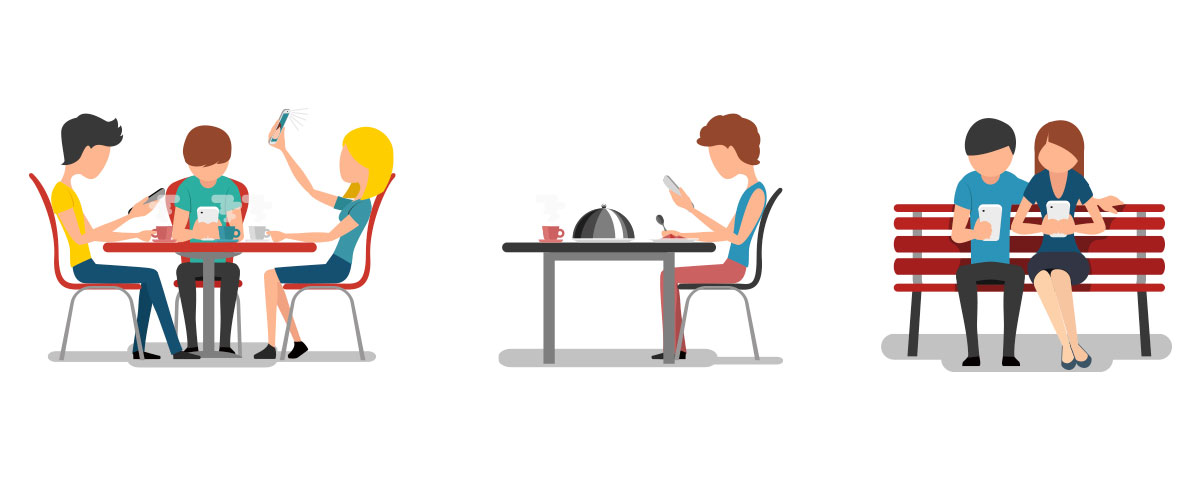
\includegraphics[width=0.48\textwidth,height=\textheight]{media/articulo09_image2.jpeg}}

\End{centerimageenv}

\Begin{smalltextenv}

\textbf{Imagen 1:} Personas utilizando dispositivos electrónicos en actividades cotidianas del ser humano \textbf{Fuente:} \href{https://earlsfieldcapital.com/}{\emph{Earlsfield Capital}}

\End{smalltextenv}

\hypertarget{articulo09_cross03}{}
\hypertarget{articulo09_cross04}{}

Las adicciones tecnológicas forman parte de una categoría denominada ``adicciones conductibles'' o también ``no tóxicas'' \protect\hyperlink{articulo09_ref03}{{[}3{]}}. Estas adicciones son tomadas en cuenta como procesos de dependencia que son parecidos a otras adicciones como a las drogas, sexo o juegos. Este tipo de desorden es causado por el uso excesivo de todos aquellos componentes electrónicos que, de una u otra forma, hacen uso de internet.

\spacefourmilis

Un ejemplo de estos podrían ser los teléfonos celulares, tabletas, videojuegos en línea, redes sociales, streaming, etc. La desorganizada forma y el mal uso que se les da a estas tecnologías está relacionado principalmente con la cantidad exorbitante de horas que se le dedican durante las que se pierde toda percepción del tiempo. Puede pasar de ser unos simples minutos ``revisando'' las redes sociales, hasta horas perdidas por consumir contenido, que, en la mayoría de los casos, no es aprovechable ni de utilidad.

\hypertarget{articulo09_cross05}{}
\hypertarget{articulo09_cross06}{}
\spacethreemilis

Esta adicción se ha determinado que ocurre principalmente entre la adolescencia media (entre los 14 y 18 años) y el inicio de la adultez \protect\hyperlink{articulo09_ref04}{{[}4{]}}. Para identificar que una persona está sufriendo una conducta adictiva es tan fácil como notar un grupo de características de cambio. Entre ellas se encuentra: pérdida de control, falta de tolerancia, pérdida de interés por otras actividades que son de interés o que generan algún tipo de gratitud y la interferencia en el flujo de la vida cotidiana \protect\hyperlink{articulo09_ref05}{{[}5{]}}. Un ejemplo que encapsula de una manera idónea esas características son los adolescentes que se vuelven adictos a los videojuegos, como por ejemplo, Fortnite. Este es un videojuego en línea desarrollado por Epic Games y lanzado en 2017 \protect\hyperlink{articulo09_ref06}{{[}6{]}}. El auge de este videojuego, debido a sus llamativos personajes, modos de juego y demás, expertos en Estados Unidos han afirmado que este videojuego puede ser tan adictivo como la heroína \protect\hyperlink{articulo09_ref06}{{[}6{]}}. La empresa Epic Games reveló que, durante el mes de agosto de 2019, el famoso videojuego fue jugado por casi 80 millones de personas durante ese mes \protect\hyperlink{articulo09_ref06}{{[}6{]}}. Una persona que es adicta a los videojuegos, como Fortnite, tiende a perder el control cuando pierde, y esto provoca que se pierda el interés en actividades como la escuela o la relación en familia.

\spacefivemilis

\Begin{centerimageenv}

\href{https://neural.es/wp-content/uploads/2018/11/fortnite-dest.jpg/}{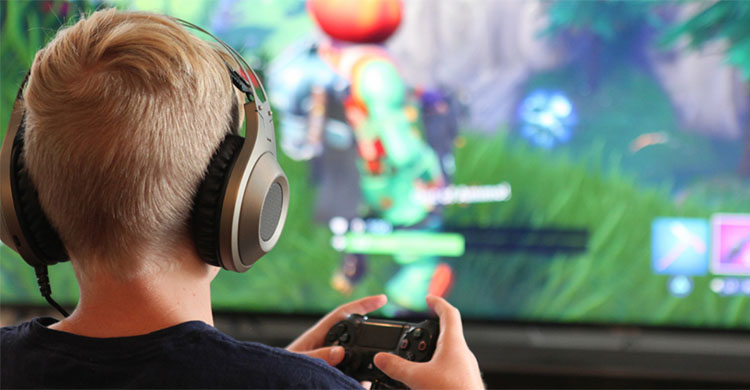
\includegraphics[width=0.48\textwidth,height=\textheight]{media/articulo09_image3.jpeg}}

\End{centerimageenv}

\Begin{smalltextenv}

\textbf{Imagen 2:} Niño jugando Fortnite \textbf{Fuente:} \href{https://neural.es/}{\emph{Clínicas Neural}}

\End{smalltextenv}

\hypertarget{quuxe9-hace-a-la-tecnologuxeda-ser-tan-adictiva}{%
\section{¿Qué hace a la tecnología ser tan adictiva?}\label{quuxe9-hace-a-la-tecnologuxeda-ser-tan-adictiva}}

\hypertarget{articulo09_cross07}{}
\hypertarget{articulo09_cross08}{}

Toda nueva tecnología representa en un adoles-
cente el tener la capacidad de abstraer su realidad a un mundo imaginario de fantasía para ignorar su vida. A través de plataformas como redes sociales, videojuegos e internet, los adolescentes tienden a mostrarse de una forma en la que no son ellos en realidad. Esa imagen ficticia de ellos mismos llega a interpretarse como una ``baja autoestima'' y este puede llegar a ser un problema psicológico en potencia. Toda falta de seguridad que presente una persona en sí mismo y esta sea sustituida por las tecnologías es una clara señal de que la persona se encuentra afectada emocionalmente y eso la vuelve vulnerable ante cualquier tipo de discriminación o cualquier otro factor que afecte su entorno.

\spacetwomilis

La tecnología satisface la necesidad humana natural de estimulación, interacción y cambios en el medio ambiente con gran eficiencia. Cuando los adolescentes experimentan estrés, ya sea el rechazo romántico o una mala calificación en un examen, la tecnología puede convertirse en una forma rápida y fácil de satisfacer las necesidades básicas y, como tal, puede volverse adictiva \protect\hyperlink{articulo09_ref07}{{[}7{]}}. La tecnología impacta los sistemas de placer del cerebro como lo harían otro tipo de adicciones como el alcohol o las drogas. La tecnología se vuelve adictiva cuando alcanza el punto en el que destruye el aburrimiento, funciona como un tipo de bálsamo social y un escape de la realidad.

\Begin{centerimageenv}

\href{https://www.lasdrogas.info/wp-content/uploads/2018/10/adiccio-tecnologia.jpg/}{
\includegraphics[width=0.48\textwidth,height=\textheight]{media/articulo09_image4.jpeg}}

\End{centerimageenv}

\Begin{smalltextenv}

\textbf{Imagen 3:} Persona manifestando un tipo de frustración, el cual es provocado por la saturación de información que encuentra en la red \textbf{Fuente:} \href{https://www.lasdrogas.info/}{\emph{lasdrogas.info}}

\End{smalltextenv}

\hypertarget{tipos-de-adicciones-tecnoluxf3gicas}{%
\section{Tipos de adicciones tecnológicas}\label{tipos-de-adicciones-tecnoluxf3gicas}}

Un periodista de datos británico llamado David McCandless realizó un estudio sobre los tipos de desórdenes de conducta provocados por la tecnología \protect\hyperlink{articulo09_ref08}{{[}8{]}}, entre los cuales se destacan los siguientes:

\begin{itemize}
\item
  \textbf{Smart Tick (Adicción al móvil):} este desorden de conducta se destaca como un problema de salud social. Todos aquellos usuarios que tienen un dispositivo móvil o smartphone tienden a tener un patrón constante de revisión por nuevas notificaciones o simplemente estar conectados todo el tiempo. Esto los hace perder la noción sobre el entorno en el que se encuentran actualmente, como puede ser una reunión, una película, una comida familiar, etc.
\item
  \textbf{Dingeing:} este desorden de conducta recibe su nombre por las palabras en inglés ``digital bingeing'' que se refiere al uso constante del botón de encendido o desbloqueo de un móvil luego de haber pasado un tiempo sin revisarlo \protect\hyperlink{articulo09_ref08}{{[}8{]}}. Se dice que el usuario atesora tanto ese momento de forma implícita que ha llegado a ser comparado como el reencuentro con un viejo amigo.
\item
  \textbf{Backlog depresión:} este desorden de conducta está orientado a todos los usuarios que tienen acceso a teléfonos móviles, tabletas y computadores. Se dice que la persona experimenta lapsos de estrés y depresión al saber que no tiene acceso a revisar sus mensajes o correos acumulados \protect\hyperlink{articulo09_ref08}{{[}8{]}}, lo cual incrementa todos sus niveles de ansiedad y recuperar la calma se le hace una tarea muy difícil.
\item
  \textbf{Divorcio digital:} este, en comparación con los otros desórdenes, es el más común y el que más se ve frecuentemente. Está asociado a toda aquella actividad, ya sea en pareja o en familia, en la que todos los miembros se encuentran revisando sus dispositivos móviles sin cruzar una sola palabra. Este tipo de comportamiento muestra que el revisar un dispositivo llega a ser más importante que una conversación entre personas.
\end{itemize}

\Begin{centerimageenv}

\href{https://okdiario.com/img/tecnologia/2015/03/adictos-2.jpg/}{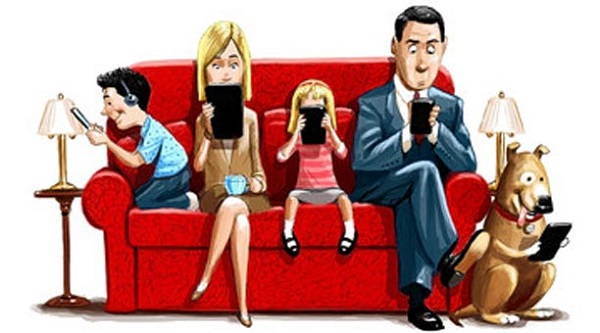
\includegraphics[width=0.48\textwidth,height=\textheight]{media/articulo09_image5.jpeg}}

\End{centerimageenv}

\Begin{smalltextenv}

\textbf{Imagen 4:} Familia, durante un tiempo de convivencia, utilizando dispositivos móviles \textbf{Fuente:} \href{https://okdiario.com/img/tecnologia/2015/03/adictos-2.jpg}{\emph{okdiario}}

\End{smalltextenv}

\hypertarget{cuxf3mo-prevenir-las-adicciones-tecnoluxf3gicas}{%
\section{¿Cómo prevenir las adicciones tecnológicas?}\label{cuxf3mo-prevenir-las-adicciones-tecnoluxf3gicas}}

La tecnología se caracteriza por su inevitable crecimiento. Es difícil pensar en que la tecnología no va a seguir creciendo para el mundo de los adolescentes y por ello es importante prevenir el consumo obsesivo de ella únicamente se puede afrontar encontrando algún tipo de equilibrio. El principal objetivo por atacar, para solucionar este tipo de adicción es evitando que los más jóvenes utilicen la tecnología como un escape de los desafíos, las emociones y la socialización \protect\hyperlink{articulo09_ref07}{{[}7{]}}. Algunas de las formas en las que se puede llegar a tener una relación saludable con la tecnología es aplicando algunas de las siguientes técnicas:

\begin{itemize}
\item
  \textbf{Proveer actividades de plenitud:} esta técnica consiste en incentivar a los jóvenes a preferir actividades recreativas sobre algunas que involucren tecnología. Cada vez que un hijo, amigo, hermano esté a punto de jugar algún videojuego o utilizar un dispositivo electrónico, invitarlo a realizar alguna actividad que involucre su persona como salir a caminar, practicar algún deporte, etc.
\item
  \textbf{Balancear la actividad y productividad con estrés sano:} todo en la vida requiere energía y muy seguido sucede que los adolescentes sienten que tienen muy poca de ella para invertirla en algunas actividades \protect\hyperlink{articulo09_ref07}{{[}7{]}}. Con la tutela de un adulto, los adolescentes pueden llegar a descubrir formas saludables para reponer esa energía. Esto puede ser una solución factible para el fácil alivio de estrés que provoca la adicción a la tecnología.
\item
  \textbf{Fomentar el desarrollo de la identidad en el mundo real:} gran parte de como se comporta un adolescente tiene que ver con la crianza de sus padres. Si estos últimos en vez de utilizar tecnología como herramienta de distracción en sus hijos, los incentivan a encontrar algo en lo que sean buenos y los motiven a que quieran hacerlo van a poder encontrar un escape sano de esta adicción. El mundo necesita cultivar más propósitos e identidades en los jóvenes dentro del círculo familiar e incluso en escuelas y comunidades.
\end{itemize}

\Begin{centerimageenv}

\href{http://www.rethinkya.com/wp-content/uploads/2017/08/no-tenemos-wifi-hablen-entre-ustedes.jpg/}{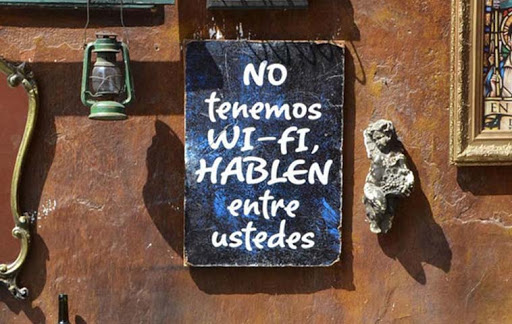
\includegraphics[width=0.45\textwidth,height=\textheight]{media/articulo09_image6.jpeg}}

\End{centerimageenv}

\Begin{smalltextenv}

\textbf{Imagen 4:} Publicidad en un bar que fomenta la comunicación entre personas dejando a un lado los dispositivos que se conectan a internet. El mensaje indica ``No tenemos WiFi, hablen entre ustedes'' \textbf{Fuente:} \href{http://www.rethinkya.com/}{\emph{Rethinkya}}

\End{smalltextenv}

\hypertarget{conclusiones-8}{%
\section*{Conclusiones}\label{conclusiones-8}}
\addcontentsline{toc}{section}{Conclusiones}

\begin{itemize}
\item
  Se determinó que una adicción tecnológica puede ser igual o peor que la adicción a las drogas o al alcohol. La tecnología es una línea que tiende al infinito, nunca se sabe que puede venir después y como esta puede afectar a los que nos rodean. Lo importante de saber que la tecnología crece es que se debe aprovechar dándole un uso sano y controlado, ya sea por iniciativa propia o por el control de los padres (en caso de los adolescentes).
\item
  Se determinó los diferentes tipos de adicciones tecnológicas más comunes que existen. Estas, en su mayoría, se presentan de una forma inesperada entre todos aquellos usuarios que por primera vez experimentan el uso de la tecnología como un medio para satisfacer sus necesidades diarias. Es importante identificar cada una de ellas para poderlas tratar y reconocer que afectan indirectamente tanto nuestra actitud y comportamiento como nuestras relaciones interpersonales.
\item
  Se determinó que existen diferentes formas de tratar las adicciones tecnológicas y que estas no requieren cambios extremadamente pronunciados en nuestras actividades. Estos cambios únicamente dependen del rol que se esté empleando. Para los padres de familia que cuentan con hijos adolescentes, es importante incentivarlos a practicar actividades recreativas que los mantengan un poco alejados de la tecnología. Para los adultos, es necesario identificar los momentos en los que no se debería de hacer uso de tecnología para no afectar las actividades naturales como ser humano.
\end{itemize}

\hypertarget{referencias-8}{%
\section*{Referencias}\label{referencias-8}}
\addcontentsline{toc}{section}{Referencias}

\begin{itemize}
\item
  \hypertarget{articulo09_ref01}{}

  \protect\hyperlink{articulo09_cross01}{{[}1{]}} \href{https://www.healthline.com/}{«Healthline»}, \href{https://www.healthline.com/health/addiction}{What Is Addiction?}, 11 octubre 2019. {[}En línea{]}. Disponible en: \url{https://bit.ly/32ArJPT}. {[}Último acceso: 09 marzo 2020{]}.
\item
  \hypertarget{articulo09_ref02}{}

  \protect\hyperlink{articulo09_cross02}{{[}2{]}} Nick Waddell \href{https://www.cantechletter.com/}{«Cantech Letter»}, \href{https://www.cantechletter.com/2013/01/what-is-technology0103/}{What is technology?}, 29 marzo 2019. {[}En línea{]}. Disponible en: \url{https://bit.ly/2E8yrlV}. {[}Último acceso: 09 marzo 2020{]}.
\item
  \hypertarget{articulo09_ref03}{}

  \protect\hyperlink{articulo09_cross03}{{[}3{]}} Julia Smith \href{https://www.sandstonecare.com/}{«Sandstone Care»}, \href{https://www.sandstonecare.com/resources/substance-abuse/technology-addiction}{Technology Addiction - Teen \& Young Adult \textbar{} Sandstone Care}, 19 septiembre 2018. {[}En línea{]}. Disponible en: \url{https://bit.ly/2CC2X79}. {[}Último acceso: 09 marzo 2020{]}.
\item
  \hypertarget{articulo09_ref04}{}

  \protect\hyperlink{articulo09_cross04}{{[}4{]}} Maite Nicueza Guelbenzu \href{https://www.webconsultas.com/}{«Webconsultas»}, \href{https://www.webconsultas.com/mente-y-emociones/adicciones/por-que-somos-adictos-a-internet}{Adicción a Internet y las tecnologías}, 14 julio 2020. {[}En línea{]}. Disponible en: \url{https://bit.ly/3hmsQGX}. {[}Último acceso: 09 marzo 2020{]}.
\item
  \hypertarget{articulo09_ref05}{}

  \protect\hyperlink{articulo09_cross05}{{[}5{]}} \href{http://www.aprovat.org/}{«Aprovat»}, \href{http://www.aprovat.org/adicciones-tecnologicas/}{ADICCIONES TECNOLÓGICAS - Aprovat Adicciones}, 23 enero 2014. {[}En línea{]}. Disponible en: \url{https://bit.ly/3fUNgGI}. {[}Último acceso: 10 marzo 2020{]}.
\item
  \hypertarget{articulo09_ref06}{}

  \protect\hyperlink{articulo09_cross06}{{[}6{]}} Asmir Pekmic \href{https://www.vgr.com/}{«VGR»}, \href{https://www.vgr.com/fortnite-is-as-addictive-as-heroin-according-to-health-experts/}{Fortnite Is As Addictive As Heroin According To Health Experts}. {[}En línea{]}. Disponible en: \url{https://bit.ly/2ONCYw2}. {[}Último acceso: 09 marzo 2020{]}.
\item
  \hypertarget{articulo09_ref07}{}

  \protect\hyperlink{articulo09_cross07}{{[}7{]}} \href{https://www.hazeldenbettyford.org/}{«Hazeldenbettyford»}, \href{https://www.hazeldenbettyford.org/articles/fcd/teen-technology-addiction/}{Technology Addiction}, 16 marzo 2017. {[}En línea{]}. Disponible en: \url{https://bit.ly/2Cu4FYu}. {[}Último acceso: 09 marzo 2020{]}.
\item
  \hypertarget{articulo09_ref08}{}

  \protect\hyperlink{articulo09_cross08}{{[}8{]}} \href{https://prnoticias.com/}{«Prnoticias»}, \href{https://prnoticias.com/podcast/ondacro/tendencias-tecnologicas/20154619-acciones-tecnologia-internet/}{8 tipos de adicciones a la tecnología e Internet que padeces sin saberlo}, 06 julio 2016. {[}En línea{]}. Disponible en: \url{https://bit.ly/3jt8OML}. {[}Último acceso: 09 marzo 2020{]}.
\end{itemize}

\Begin{centerimageenv}

\href{https://dtt-ecys.org}{
\includegraphics[width=0.3\textwidth,height=\textheight]{media/logo_50.png}}

\End{centerimageenv}

\End{multicols}

\titleformat{\chapter}[block]{\formatchapterEdDQ}{\labelchapterEdDQ}{195pt}{\beforecodechapterEdDQ#1\beforecodechapterparttwoEdDQ}

\titlespacing*{\chapter} {\leftchapterEdDQ}{\beforesepchapterEdDQDobleLine}{\afterchapterEdDQDobleLine}

\titleformat{\section}[block]{\formatsection}{\labelsection}{\sepsection}{\beforecodesection#1}

\titleformat{\subsection}[block]{\formatsubsection}{\labelsubsection}{\sepsubsection}{\beforecodesubsection#1}

\titleformat{\subsubsection}[block]{\formatsubsubsection}{\labelsubsubsection}{\sepsubsubsection}{\beforecodesubsubsection#1}

\hypertarget{article10}{%
\chapter{Cloud computing, modelos de capa gratuita como oportunidad de aprendizaje y capacitación}\label{article10}}

\BeginKnitrBlock{photobiography3}{media/articulo10_image1.png}
\begin{styleAuthorName}

Pablo Andrés Hernández Rivera

\end{styleAuthorName}

\begin{styleAuthormail}

\href{mailto:hpablo677@gmail.com}{\nolinkurl{hpablo677@gmail.com}}

\end{styleAuthormail}

Estudiante de Ingeniería en Ciencias y Sistemas - USAC

\begin{styleKeywords}

\textbf{Palabras Clave:}\\
Cloud Computing, AWS, Google Cloud Computing, Azure, Marketing, capacitación, modelos de negocio.

\end{styleKeywords}
\EndKnitrBlock{photobiography3}

\Begin{multicols}{2}
\hypertarget{articulo10_cross01}{}

\hypertarget{marketing-y-sus-estrategias}{%
\section{Marketing y sus estrategias}\label{marketing-y-sus-estrategias}}

A lo largo de la historia distintas estrategias de marketing han sabido cautivar a potenciales consumidores de un producto o servicio. Estas han ido evolucionando según la necesidad y capacidad del producto para entrar en nuevos mercados, pero ¿cómo se da a conocer un producto nuevo? Las estrategias y técnicas de mercadeo han sido desarrolladas a lo largo del tiempo siendo el conjunto de prácticas y principios que tienen como objetivo aumentar el comercio lo que se denomina Mercadotecnia. Una de las técnicas más comunes de la mercadotecnia es la muestra gratis. Es natural desconfiar de un producto cuando se le desconoce, por ello los comercializadores del producto tienen la obligación de darlo a conocer ante los consumidores para generar demanda. Con este principio, se han diseñado modelos de comercialización de muestra o prueba gratuita de productos y servicios, para atraer a nuevos consumidores quienes al principio se muestran inseguros de la calidad y desempeño de estos. El modelo ha demostrado ser un medio de mercadeo con notables aspectos positivos tales como: preferencia del cliente, retroalimentación y divulgación; interés nuevo por el producto; y generación de necesidad.

\hypertarget{productos-de-software-y-estrategias-de-marketing}{%
\section{Productos de software y estrategias de marketing}\label{productos-de-software-y-estrategias-de-marketing}}

Como modelo de negocios, la muestra gratuita es efectiva para demandas de productos específicos, pero ¿cómo ha resultado con los productos de software? Desde la comercialización de las computadoras, el concepto de licenciamiento y adquisición de nuevo software ha sido el ingreso principal de las compañías desarrolladoras. A lo largo del tiempo, se han adaptado normas y reglas que beneficien de la mejor manera a ambas partes: consumidores y proveedores de productos de software. Existen muchos aspectos a considerar en cuanto a comercialización de software: acuerdos de privacidad; términos y condiciones de uso; tipos de licencia; tipos de cuenta; y distribuciones que limiten las funcionalidades y el soporte. Dado que distintas empresas desarrolladoras se han visto envueltas en conflictos legales se han visto obligadas a tener que especificar hasta el mínimo término, para protegerse de usuarios que hacen un uso indebido de sus aplicaciones al compartir los datos de la aplicación y descifrando los ejecutables para que puedan usarse libremente. En consecuencia de las restricciones legales establecidas, han surgido movimientos sociales y filosofías de trabajo, como ``el movimiento de software libre de los años 80'' \protect\hyperlink{articulo10_ref01}{{[}1{]}}, o las condenas por piratería de software y multas que infringen distintos gobiernos, por ser un daño o perjuicio hacia las empresas y su producto.

El valor de los productos de software está sujeto a las necesidades y preferencias del usuario como en cualquier otro producto. De aquí que las empresas de software se hayan visto en la necesidad de adquirir distintos modelos de negocio y publicidad, que les permitan atraer nuevos usuarios y personas dispuestas a hacer uso de su producto antes que otras, y dado que el software es uno de los mercados más grandes, atractivos y competitivos, no es algo que se tome a la ligera.

\Begin{centerimageenv}

\href{https://www.spotify.com/gt/}{
\includegraphics[width=0.48\textwidth,height=\textheight]{media/articulo10_image4.png}}

\End{centerimageenv}

\Begin{smalltextenv}

\textbf{Imagen 1:} Página principal de Spotify \textbf{Fuente:} \href{https://www.spotify.com/gt/}{\emph{Spotify}}

\End{smalltextenv}

\spaceminusmilis

Eventualmente, se tomó la decisión de adoptar el modelo publicitario de la muestra gratis en los productos de software, sin embargo, se optó por limitar el uso de las herramientas de software de forma tal que brindaran al usuario una experiencia lo suficientemente completa pero sin comprometerlo con eventuales conflictos de piratería.
Muchas versiones de la muestra gratis han sido implementadas en software como por ejemplo:

\spaceminusmilis

\begin{itemize}
\item
  Funciones limitadas, en donde el usuario tiene acceso solo a ciertas funcionalidades, para hacer uso de opciones avanzadas tiene que adquirir licencia.
\item
  Periodo de tiempo, en donde el usuario solo dispone de una cantidad de días para utilizar la aplicación hasta que esta se bloquee.
\item
  Modelo de anuncios publicitarios, donde el usuario puede usar la aplicación de manera gratuita, pero se ve constantemente interrumpido por comerciales.
\item
  Mixtos, entre todos los modelos anteriores.
\end{itemize}

\spaceminusmilis

A pesar de los distintos diseños de publicidad de muestra gratuita implementados en los productos de software, siempre se han presentado inconvenientes para controlar al usuario en los límites que define el concepto de prueba. Las personas han encontrado la manera de evadir los bloqueos de las empresas desarrolladoras para permitirse seguir utilizando la aplicación sin pagar, o han preferido soportar los anuncios antes que desembolsar alguna cantidad monetaria. Esto puede deberse a la cultura de comercio de cada usuario y el valor que tiene para él la aplicación. Recientemente un nuevo modelo de negocios ha acaparado el mercado debido a la tendencia del internet, este nuevo modelo es: la nube.

\Begin{centerimageenv}

\href{https://www.winrar.es/comprar}{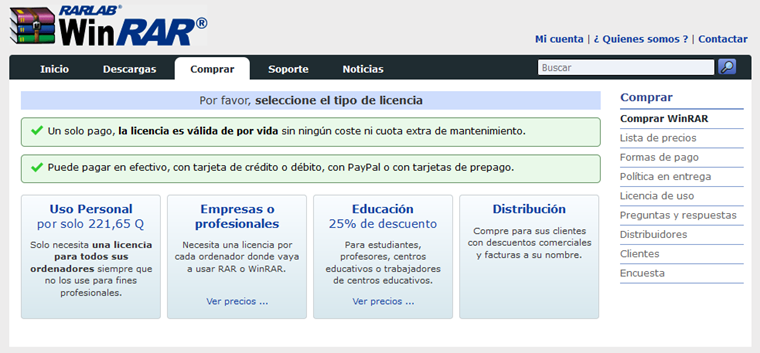
\includegraphics[width=0.48\textwidth,height=\textheight]{media/articulo10_image5.png}}

\End{centerimageenv}

\Begin{smalltextenv}

\textbf{Imagen 2:} Precios de WinRAR \textbf{Fuente:} \href{https://www.winrar.es/comprar}{\emph{Winrar}}

\End{smalltextenv}

\hypertarget{la-nube-y-modelos-de-capa-gratuita-como-estrategia-de-marketing}{%
\section{La nube y modelos de capa gratuita como estrategia de marketing}\label{la-nube-y-modelos-de-capa-gratuita-como-estrategia-de-marketing}}

La nube es el concepto de usar aplicaciones de internet para realizar tareas, en lugar de realizarlas usando el hardware del que se dispone. Estas aplicaciones van desde almacenamiento hasta infraestructuras completas. Esta tecnología habilita el consumo de sus servicios con diversas características mucho más convenientes. Bajo este modelo se paga por lo que se consume, además introduce nuevos conceptos de definición de requerimientos: la escalabilidad, la elasticidad, flexibilidad, y disponibilidad. Todo esto está disponible desde cualquier lugar con acceso a internet, por medio de un portal de auto aprovisionamiento. La nube, como tecnología, tiene un futuro prometedor, mientras que el uso de software para uso personal y empresarial está disminuyendo gracias a las ventajas de los modelos de pago que ofrece y la variedad de los servicios disponibles. La nube tiene una ventaja superior a la hora de ofrecer un sistema de publicidad de prueba gratuita debido a que el usuario no posee lo que está en la nube, únicamente hace uso del servicio. Bajo esta premisa, el usuario no tiene oportunidad de hacer uso indebido de las aplicaciones y se ve envuelto en la dependencia de la herramienta que escoja.

\spacefourmilis

Pero toda tecnología tiene que ser manipulada. Desde el principio de la computación, ha sido labor de gente capacitada el uso de estas herramientas tecnológicas. Las empresas han desarrollado productos de software que requieren de cierto entendimiento único y las personas que se ven necesitadas de usar una aplicación deben pasar por un largo proceso de aprendizaje, tal y como se haría en cualquier otra profesión y con cualquier otra herramienta de trabajo. Conforme la popularidad de las herramientas ha incrementado, y se ha generado dependencia por parte de las empresas con el uso de un sistema, más personas deben pasar por este proceso de aprendizaje. Si las empresas brindan la oportunidad de utilizar sus herramientas como prueba del producto y las personas tienen necesidad de aprender a usar estos productos, ¿qué tanto puede explotarse el modelo de marketing para capacitar a una persona?

\hypertarget{proveedores-de-servicios-en-la-nube-y-sus-modelos-de-capa-gratuita}{%
\section{Proveedores de servicios en la nube y sus modelos de capa gratuita}\label{proveedores-de-servicios-en-la-nube-y-sus-modelos-de-capa-gratuita}}

Evaluando las ventajas y opciones que ofrecen distintos proveedores de servicios en la nube, es notable que las opciones son prácticamente ilimitadas a la hora de introducirse en lo que puede necesitar una empresa de tecnología por parte de un nuevo aspirante. Las opciones de capa gratuita de un modelo de negocios en la nube van desde inteligencia artificial, hasta bases de datos y servidores, con facilidad de disponibilidad y soporte constante. Concretamente, en este artículo se analizarán 3 servicios de tecnología en la nube: Google Cloud Platform (GCP), Amazon AWS, y Microsoft Azure.

\hypertarget{articulo10_cross02}{}

GCP consta de ``un conjunto de recursos físicos, como computadoras y unidades de disco duro, y virtuales, como las máquinas virtuales (VM), que se encuentran en los centros de datos de Google de todo el mundo''. \protect\hyperlink{articulo10_ref02}{{[}2{]}} Cada centro de datos está ubicado en una región global. Estas incluyen el centro de USA, Europa occidental y Asia oriental. Cada región es una colección de zonas aisladas entre sí dentro de cada región.

\Begin{centerimageenv}

\href{https://cloud.google.com/docs/images/overview/regions-zones.svg?hl=es-419/}{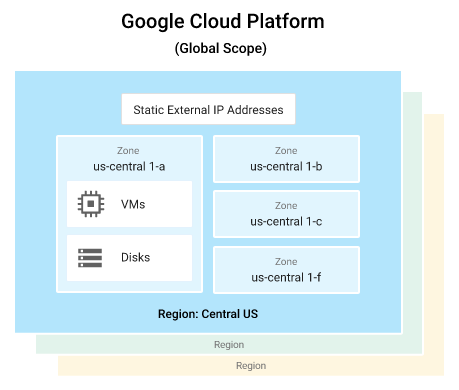
\includegraphics[width=0.48\textwidth,height=\textheight]{media/articulo10_image7.png}}

\End{centerimageenv}

\Begin{smalltextenv}

\textbf{Imagen 3:} Alcance general de GCP \textbf{Fuente:} \href{https://cloud.google.com/}{\emph{Google}}

\End{smalltextenv}

\hypertarget{articulo10_cross03}{}

Amazon Web Services (AWS) es la plataforma en la nube más adoptada y completa en el mundo, que ofrece más de 175 servicios integrales de centros de datos a nivel global. ``Cuenta con millones de clientes, incluyendo las empresas emergentes que crecen más rápido, las compañías más grandes y los organismos gubernamentales líderes, quienes utilizan AWS para reducir los costos, aumentar su agilidad e innovar de forma más rápida''. \protect\hyperlink{articulo10_ref03}{{[}3{]}}

\hypertarget{articulo10_cross04}{}

Azure es un conjunto completo y en expansión constante de servicios de informática en la nube. ``Ofrece flexibilidad de crear, administrar e imple-
mentar aplicaciones en una red mundial enorme con las herramientas y las plataformas que proporciona Microsoft''. \protect\hyperlink{articulo10_ref04}{{[}4{]}}

\hypertarget{articulo10_cross05}{}

Estas herramientas pueden ubicarse como las más populares según ``el cuadrante mágico de Gartner'' \protect\hyperlink{articulo10_ref05}{{[}5{]}}, el cual posiciona tecnologías en mercados específicos según liderazgo y visión:

\Begin{centerimageenv}

\href{https://pages.awscloud.com/rs/112-TZM-766/images/MQ-transparent.png/}{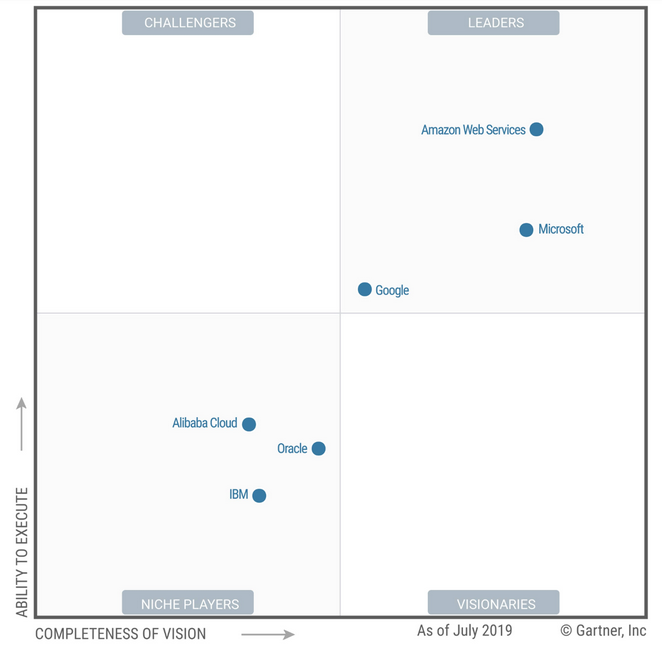
\includegraphics[width=0.48\textwidth,height=\textheight]{media/articulo10_image8.png}}

\End{centerimageenv}

\Begin{smalltextenv}

\textbf{Imagen 4:} Cuadrante mágico de Gartner \textbf{Fuente:} \href{https://pages.awscloud.com/}{\emph{Gartner, Inc.}}

\End{smalltextenv}

A continuación, se describen las opciones que ofrece la capa gratuita de cada plataforma en la nube, hacia marzo del año 2020:

\hypertarget{articulo10_cross06}{}
\hypertarget{articulo10_cross07}{}
\hypertarget{articulo10_cross08}{}

\textbf{GCP:} proporciona todas sus herramientas y funcionalidades, con un límite de inversión de los primeros \$300.00 USD sin costo. Una vez los gastos en las herramientas sobrepasan este valor, se empieza a cobrar. Para hacer uso de la GCP, se requiere una cuenta de Google y una tarjeta de crédito: ``GCP cuenta con más de 100 productos de tecnología en la nube, que se pueden clasificar en: IA, administración de APIs, procesamiento, contenedores, análisis de datos, bases de datos, herramientas de desarrollo, salud y ciencias biológicas, nubes híbridas y múltiples, internet de las cosas, administración, multimedia, videojuegos, migración de datos, redes, seguridad, serverless, y almacenamiento''. \protect\hyperlink{articulo10_ref06}{{[}6{]}} La ventaja de limitar la cantidad de dinero que puede invertirse permite al usuario administrarse de la forma que prefiera, e invertir únicamente en un servicio si lo desea.

\textbf{AWS:} ofrece limitantes en sus funcionalidades según el uso para empezar a cobrar. Todos los servicios de AWS tienen un costo por hora o uso bien definido. La capa gratuita de AWS dura 12 meses, con el concepto de renovación cada 30 días para los límites de las funciones: Si se sobrepasan en uso, pueden empezar a cobrar por el mismo dentro de los 30 días, pero reiniciar a la capa gratuita a los 30 días siguientes. Esto limita al usuario a llevar un control de lo que utiliza cada 30 días, independientemente del servicio y costo individual. ``Ofrece servicios de análisis, integración, RA, RV, productividad empresarial, informática, servicio al cliente, base de datos, herramientas de desarrollo, informática de usuarios finales, videojuegos, internet de las cosas, machine learning, administración, multimedia, aplicaciones móviles, red, robótica, seguridad y almacenamiento''. \protect\hyperlink{articulo10_ref08}{{[}8{]}} Cuenta con muchas más herramientas que ningún otro servicio en la nube, ya que es, en realidad, el primer servicio de tecnologías de este tipo, y, por ende, líder y pionera en el ámbito. Si bien puede ser conocida por tener modelos de costos más elevados que la competencia, tiene mucha demanda en el mercado y confianza por parte de empresas que ya alojan toda su infraestructura en AWS.

\textbf{Azure:} es una plataforma que ha adquirido mucha popularidad en los últimos tiempos, debido a la dependencia a Microsoft que existe por parte de la mayoría de las empresas y desarrolladores, al ser Windows uno de los sistemas operativos preferidos por usuarios finales. Su modelo de capa gratuita es quizá el más completo, al incluir por 12 meses, \$200 USD mensuales en costos para probar las herramientas más populares. Sin embargo, existen 25 herramientas que son gratuitas siempre. Los servicios que ofrecen son: ``Máquinas virtuales, análisis de datos, moderación de servicios, IA, almacenamiento, bases de datos, red, internet de las cosas, serverless, manejo de APIs, contenedores, seguridad, herramientas de desarrollo, aplicaciones móviles, automatización y administración''. \protect\hyperlink{articulo10_ref08}{{[}8{]}}

\spaceminusmilis

Todos los modelos anteriores ofrecen muchos servicios indispensables para cualquier empresa que quiera estar a la vanguardia y brindar un buen servicio, pero es tanta información, que para una persona es muy difícil aprovechar al máximo cada una, y, por ende, representar una pérdida real para los proveedores de tecnologías en la nube. Si bien, una empresa pequeña puede iniciar usando únicamente la capa gratuita, eventualmente se verá limitada por esta. Y si una empresa crece dentro de la capa gratuita, deberá seguir una vez finalizado su plazo si no quiere verse en la tarea de migrar toda su infraestructura. Esto es comparable con una persona que crea una cuenta y adquiere un periodo de prueba en Netflix. Si bien, podrá disfrutar un tiempo del contenido, no le alcanzarían 30 días de prueba para ver todo el contenido del que dispone. \protect\hyperlink{articulo10_ref08}{{[}8{]}}

Sin embargo, una persona con cierta preparación en el mundo de la computación, quien es el usuario objetivo de las tecnologías en la nube, puede registrarse en la plataforma y aprender a usarla en el periodo de tiempo de la capa gratuita. Independientemente de si tiene interés en la tecnología o tiene necesidad de capacitarse por su profesión, la capa gratuita es una oportunidad increíblemente grande de preparación para certifi-
carse como experto en las herramientas que ofrece. Posteriormente, su perfil sería mucho más elevado que el de alguien que no tiene preparación en las herramientas, y tendría mayor oportunidad de desempeñarse como profesional en la nube. Este es un perfil cada vez más cotizado por las empresas. Conociendo los modelos de capa gratuita que ofrecen los proveedores líderes, es razonable buscar una especialización en la mayoría de los servicios.

\hypertarget{conclusiones-9}{%
\section*{Conclusiones}\label{conclusiones-9}}
\addcontentsline{toc}{section}{Conclusiones}

\begin{itemize}
\tightlist
\item
  Los productos de software adoptan modelos de marketing para promoverse entre los potenciales usuarios, quienes gozan de un gran beneficio en probar los mismos productos antes de decidir si es lo que necesitan o no.
\end{itemize}

\spaceonemilis

\begin{itemize}
\tightlist
\item
  La nube es la tendencia más grande en tecnología y por su popularidad, le es oportuno implementar el modelo de prueba gratuita para atraer a nuevos usuarios.
\end{itemize}

\spaceonemilis

\begin{itemize}
\tightlist
\item
  A las empresas les interesa tener gente capacitada para usar sus herramientas y como cada día más empresas trasladan su infraestructura a la nube, estas buscan contratar personas con el perfil para manejo de estas.
\end{itemize}

\spaceonemilis

\begin{itemize}
\tightlist
\item
  Las personas pueden optar a utilizar el modelo de capa gratuita de los proveedores de servicios en la nube, para aprender a usar estas herramientas tan importantes en la actualidad y estar a la vanguardia en su perfil profesional.
\end{itemize}

\hypertarget{referencias-9}{%
\section*{Referencias}\label{referencias-9}}
\addcontentsline{toc}{section}{Referencias}

\begin{itemize}
\item
  \hypertarget{articulo10_ref01}{}

  \protect\hyperlink{articulo10_cross01}{{[}1{]}} \href{https://www.gnu.org/}{«GNU»}, \href{https://www.gnu.org/philosophy/philosophy.html}{Philosophy of the GNU Project}, 15 septiembre 2019. {[}En línea{]}. Disponible en: \url{https://bit.ly/3fT2xrn}. {[}Último acceso: 14 marzo 2020{]}.
\item
  \hypertarget{articulo10_ref02}{}

  \protect\hyperlink{articulo10_cross02}{{[}2{]}} \href{https://cloud.google.com/}{«Google Cloud»}, \href{https://cloud.google.com/docs/overview?hl=es-419/}{Descripción general de Google Cloud Platform}, 10 julio 2020. {[}En línea{]}. Disponible en: \url{https://bit.ly/2D1AaIZ}. {[}Último acceso: 14 marzo 2020{]}.
  \spacefourmilis
\item
  \hypertarget{articulo10_ref03}{}

  \protect\hyperlink{articulo10_cross03}{{[}3{]}} \href{https://azure.microsoft.com/}{«Microsoft»}, \href{https://azure.microsoft.com/es-es/overview/what-is-azure/}{Qué es Azure: Servicios en la nube de Microsoft},. {[}En línea{]}. Disponible en: \url{https://bit.ly/3fTqNKc}. {[}Último acceso: 14 marzo 2020{]}.
  \spacefourmilis
\item
  \hypertarget{articulo10_ref04}{}

  \protect\hyperlink{articulo10_cross04}{{[}4{]}} \href{https://aws.amazon.com/}{«Amazon Web Services»}, \href{https://aws.amazon.com/es/what-is-aws/}{Informática en la nube con AWS}, . {[}En línea{]}. Disponible en:\url{https://amzn.to/3g5JWZD}. {[}Último acceso: 14 marzo 2020{]}.
  \spacefourmilis
\item
  \hypertarget{articulo10_ref05}{}

  \protect\hyperlink{articulo10_cross05}{{[}5{]}} \href{https://pages.awscloud.com/}{«Amazon Web Services»}, \href{https://pages.awscloud.com/Gartner-Magic-Quadrant-for-Infrastructure-as-a-Service-Worldwide.html}{Gartner Report: Magic Quadrant for Cloud Infrastructure as a Service, Worldwide (2019)}, . {[}En línea{]}. Disponible en: \url{https://bit.ly/3jynHgH}. {[}Último acceso: 14 marzo 2020{]}.
  \spacefourmilis
\item
  \hypertarget{articulo10_ref06}{}

  \protect\hyperlink{articulo10_cross06}{{[}6{]}} \href{https://cloud.google.com/}{«Google Cloud»}, \href{https://cloud.google.com/free/}{Nivel gratuito de Google Cloud Platform}, . {[}En línea{]}. Disponible en:\url{https://bit.ly/3hnhTEU}. {[}Último acceso: 14 marzo 2020{]}.
  \spacefourmilis
\item
  \hypertarget{articulo10_ref07}{}

  \protect\hyperlink{articulo10_cross07}{{[}7{]}} \href{https://aws.amazon.com/}{«Amazon Web Services»}, \href{https://aws.amazon.com/es/free/}{Capa gratuita de AWS}, . {[}En línea{]}. Disponible en:\url{https://amzn.to/2Bru9oO}. {[}Último acceso: 14 marzo 2020{]}.
  \spacefourmilis
\item
  \hypertarget{articulo10_ref08}{}

  \protect\hyperlink{articulo10_cross08}{{[}8{]}} \href{https://azure.microsoft.com/}{«Microsoft»}, \href{https://azure.microsoft.com/en-us/free/}{Create your Azure free account today}, . {[}En línea{]}. Disponible en:\url{https://bit.ly/3fNBL3P}. {[}Último acceso: 14 marzo 2020{]}.
\end{itemize}

\End{multicols}

\spaceeightmilis

\Begin{centerimageenv}

\href{http://jardin.usac.edu.gt}{
\includegraphics[width=1\textwidth,height=\textheight]{media/articulo10_image11.png}}

\End{centerimageenv}

\titleformat{\chapter}[block]{\formatchapterEdDQ}{\labelchapterEdDQ}{\sepchapterEdDQ}{\beforecodechapterEdDQ#1\beforecodechapterparttwoEdDQ}

\titlespacing*{\chapter} {\leftchapterEdDQ}{\beforesepchapterEdDQ}{\afterchapterEdDQ}

\titleformat{\section}[block]{\formatsection}{\labelsection}{\sepsection}{\beforecodesection#1}

\titleformat{\subsection}[block]{\formatsubsection}{\labelsubsection}{\sepsubsection}{\beforecodesubsection#1}

\titleformat{\subsubsection}[block]{\formatsubsubsection}{\labelsubsubsection}{\sepsubsubsection}{\beforecodesubsubsection#1}

\hypertarget{article11}{%
\chapter{La web descentralizada, un reto en internet}\label{article11}}

\BeginKnitrBlock{photobiography3}{media/articulo11_image1.png}
\begin{styleAuthorName}

Fernando Hernández Juárez

\end{styleAuthorName}

\begin{styleAuthormail}

\href{mailto:djfer.h.j@gmail.com}{\nolinkurl{djfer.h.j@gmail.com}}

\end{styleAuthormail}

Estudiante de Ingeniería en Ciencias y Sistemas - USAC

\begin{styleKeywords}

\textbf{Palabras Clave:}\\
Distribuido, comunicación, privacidad, abierta, información.

\end{styleKeywords}
\EndKnitrBlock{photobiography3}

\Begin{multicols}{2}

\hypertarget{articulo11_cross01}{}

La internet es la red de comunicación entre computadoras más utilizado actualmente del cual dependen muchos servicios personales, gubernamentales, empresariales y otros. Del uso de estos servicios por parte de los usuarios finales se derivan los datos generados para usos analíticos, marcas de tendencias y estudio de comportamientos. De aquí surgen las siguientes cuestiones: ¿Es necesario que una central de servidores de una compañía gestione completamente los datos de su aplicación? ¿Se pueden gestionar completamente y personalmente los datos propios? Es por ello que se propone la web descentralizada, un tema nuevo para el funcionamiento de la internet de hoy.
\hypertarget{articulo11_cross02}{}

\spacesixmilis

La tecnología utilizada actualmente para la publicación de aplicaciones web se denomina web 2.0. Funciona de tal manera que existe una central de servidores que procesa, transfiere y consulta los datos administrados por la aplicación. De esta forma, la compañía dueña de la aplicación, también es dueña de los datos de forma indirecta pero que puede ser utilizada según los acuerdos aceptados \protect\hyperlink{articulo11_ref01}{{[}1{]}}.

\spacesixmilis

Por otro lado, se encuentra la web 3.0, conocida como la web descentralizada. A diferencia de la web centralizada donde se depende de un servidor que procesa los datos y servicios, en esta se almacenan y procesan los datos en distintos servidores distribuidos globalmente como la interconexión de dispositivos que interactúan entre sí para llevar a cabo este proceso. Debido al uso común de dispositivos en la actualidad, es posible crear una interconexión entre estos que permiten crear una red distribuida capaz de transferir los datos entre estos puntos de acceso \protect\hyperlink{articulo11_ref02}{{[}2{]}}. De esta forma se crea una red de malla donde los datos pasan de nodo en nodo, en este caso los dispositivos, hasta llegar al destino correcto tal como se muestra en la imagen \#1.

\Begin{centerimageenv}

\href{https://www.pabloyglesias.com/wp-content/uploads/2015/03/Democracy-Device.jpg.webp}{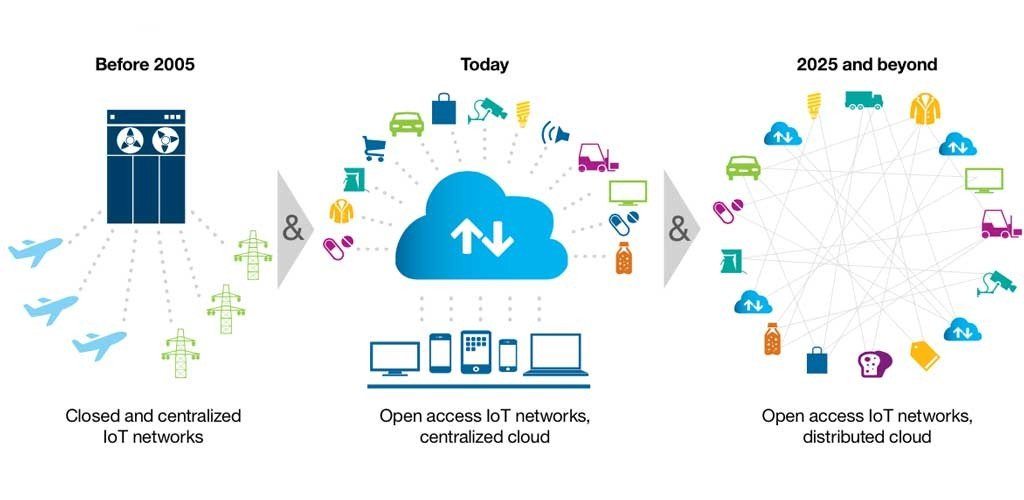
\includegraphics[width=0.48\textwidth,height=\textheight]{media/articulo11_image2.jpeg}}

\End{centerimageenv}

\Begin{smalltextenv}

\textbf{Imagen 1:} Arquitectura centralizada, centralizada en la nube y descentralizada \textbf{Fuente:} \href{https://www.pabloyglesias.com/}{\emph{pabloyglesias}}

\End{smalltextenv}

\hypertarget{articulo11_cross03}{}
\hypertarget{articulo11_cross04}{}
\hypertarget{articulo11_cross05}{}
\hypertarget{articulo11_cross06}{}
\hypertarget{articulo11_cross07}{}
\hypertarget{articulo11_cross08}{}

Utilizar esta distribución en la web ofrece control al usuario para elegir el servidor en el que se alojarán sus datos; estos datos deben ser administrados por varios servidores seleccionados. Implementar esta arquitectura web ofrece una red libre para la comunicación, la privacidad y la seguridad de los datos al proporcionarlos de forma distribuida, es decir que la información puede ser almacenada en distintos lugares a la vez. Al no existir un servidor central para la información, este es administrado por el usuario final, tal como una conexión \emph{peer-to-peer} \protect\hyperlink{articulo11_ref03}{{[}3{]}}. Actualmente existe gran cantidad de aplicaciones que implementan la web 3.0, entre estas la más conocida es Brave \protect\hyperlink{articulo11_ref04}{{[}4{]}}, un navegador web de código abierto que mejora el rendimiento, seguridad y privacidad de los datos de los usuarios.

Esta tecnología tiene beneficios para la seguridad de los datos del usuario final. Sin embargo, supone un desafío para las corporaciones que dominan la internet, ya que los datos están distribuidos de forma libre y no pueden ser usados de tal forma que se puede realizar un análisis empresarial de utilidad, y no pueden tener el control de los datos a los que acceden los usuarios y tampoco es rentable en el ámbito de negocios.

Tim Berners-Lee, creador de la \emph{World Wide Web} está trabajando en el proyecto Solid para potenciar un internet descentralizado. Solid permite crear un entorno distribuido en donde los usuarios pueden elegir el servidor que almacenará sus datos, de esta forma ninguna empresa tendrá acceso a los datos completos \protect\hyperlink{articulo11_ref05}{{[}5{]}}. Gran parte de los dominadores de internet perderían el dominio de los datos por el motivo expuesto. Estos servicios descentralizados presentan un gran reto para toda corporación que depende directamente del dominio en internet, ya que se pierde la apropiación de los datos.

Además de las aplicaciones descentralizadas ya mencionadas, existen otras en fase de implemen-
tación y producción que suponen un cambio en como utilizar la internet \protect\hyperlink{articulo11_ref06}{{[}6{]}}, entre estas figuran las siguientes:

\begin{itemize}
\item
  \textbf{Mastodon:} es una plataforma social que permite configurar la seguridad y la conexión de un servidor creado por este mismo, que se conectarán a una distribución de servidores para permitir la comunicación social de los usuarios.
\item
  \textbf{Diáspora:} es una red social compuesta de servidores distribuidos donde los usuarios eligen el servidor en el que se registrarán y de igual forma se podrán comunicar con cuentas de otros servidores.
\item
  \textbf{Matrix:} es una herramienta que permite comunicarse con otros usuarios por medio de servicios de chat en línea, voz o video ya existentes sin importar el proveedor de este servicio. Este actúa como un intermediario de comunicación entre los servicios de chat.
\item
  \textbf{Solid:} es una iniciativa de internet que permite seleccionar los datos que serán compartidos en las plataformas de internet que deseen de tal forma que se puede tener control de estos datos en internet.
\item
  \textbf{Blockstack:} es una plataforma administradora de identidad de usuarios, que permite gestionar la información que puede ser compartida y definir el acceso para externos.
\end{itemize}

Ante lo expuesto, surge la pregunta sobre si esta implementación puede ser factible debido a los requisitos de comunicación y permisividad que conlleva. Se puede decir que la descentralización de la internet permite que las aplicaciones web ofrezcan un servicio con base en los criterios del usuario final. De esta se necesita implementar la arquitectura de la internet que permita esta funcionalidad, tal como la red de mallas, cuya implementación es factible con la cantidad de dispositivos interconectados que existen actualmente. La imagen \#2 expone el cambio de lo que debe ser modificado e implementado para hacer funcionar esta tendencia de la web. En ésta se especifica la interconexión de dispositivos disponibles y dedicados para el procesamiento de la información de forma distribuida. Debe tenerse presente que se requiere una gran cantidad de dispositivos para permitir una conectividad y rendimiento óptimos.

\Begin{centerimageenv}

\href{https://101blockchains.com/wp-content/uploads/2018/09/Internet_centralizado_vs_descentralizado.jpg}{\includegraphics[width=0.48\textwidth,height=\textheight]{media/articulo11_image3.jpeg}}

\End{centerimageenv}

\Begin{smalltextenv}

\textbf{Imagen 2:} Internet centralizado vs.~Descentralizado \textbf{Fuente:} \href{https://101blockchains.com/}{\emph{101 Blockchains}}

\End{smalltextenv}

\hypertarget{conclusiones-10}{%
\section*{Conclusiones}\label{conclusiones-10}}
\addcontentsline{toc}{section}{Conclusiones}

\begin{itemize}
\item
  La implementación de una red de esta magnitud es factible actualmente por el uso común de los dispositivos con conexión a internet.
\item
  La web descentralizada provee la gestión personalizada de los datos de los usuarios, donde brinda mayor control de lo que puede ser compartido o no.
\item
  Una internet libre y abierta brinda confiabilidad al usuario final, pero afecta a las grandes organizaciones en los temas de análisis de datos.
\end{itemize}

\hypertarget{referencias-10}{%
\section*{Referencias}\label{referencias-10}}
\addcontentsline{toc}{section}{Referencias}

\begin{itemize}
\item
  \hypertarget{articulo11_ref01}{}

  \protect\hyperlink{articulo11_cross01}{{[}1{]}} Lucía Gavilán Rivillas \href{https://blogthinkbig.com/}{«Telefonica Blogthinkbig»}, \href{https://blogthinkbig.com/descentralizacion-de-la-web}{Tim Berners-Lee apuesta por la descentralización}, 09 junio 2017. {[}En línea{]}. Disponible en: \url{https://bit.ly/2D37mji}. {[}Último acceso: 13 marzo 2020{]}.
\item
  \hypertarget{articulo11_ref02}{}

  \protect\hyperlink{articulo11_cross02}{{[}2{]}} Elías Rodríguez García \href{https://www.elespanol.com/}{«El Español»}, \href{https://www.elespanol.com/omicrono/20180127/internet-descentralizado-solucion-fin-neutralidad-red/280472793_0.html/}{El Internet descentralizado, la solución al fin de la neutralidad de la red}, 27 enero 2018. {[}En línea{]}. Disponible en: \url{https://bit.ly/2OU9blj}. {[}Último acceso: 13 marzo 2020{]}.
\item
  \hypertarget{articulo11_ref03}{}

  \protect\hyperlink{articulo11_cross03}{{[}3{]}} Raúl Rustarazo \href{https://www.lainformacion.com/}{«La Información»}, \href{https://www.lainformacion.com/management/asi-es-la-web-3-0-la-red-descentralizada-que-promete-un-internet-libre-de-nuevo/6494658/}{Así es la web 3.0: la red descentralizada que promete un Internet libre de nuevo}, 12 marzo 2019. {[}En línea{]}. Disponible en: \url{https://bit.ly/2D22YkY}. {[}Último acceso: 13 marzo 2020{]}.
  \spaceminusmilis
\item
  \hypertarget{articulo11_ref04}{}

  \protect\hyperlink{articulo11_cross04}{{[}4{]}} \href{https://www.evaluandosoftware.com/}{«EvaluandoSoftware.com»}, \href{https://www.evaluandosoftware.com/dapps-piezas-basicas-la-internet-del-futuro/}{DApps: piezas básicas de la Internet del futuro}, 23 abril 2018. {[}En línea{]}. Disponible en: \url{https://bit.ly/2WLGf3B}. {[}Último acceso: 14 marzo 2020{]}.
  \spaceminusmilis
\item
  \hypertarget{articulo11_ref05}{}

  \protect\hyperlink{articulo11_cross05}{{[}5{]}} Ramón Peco \href{https://www.lavanguardia.com/}{«La Vanguardia»}, \href{https://www.lavanguardia.com/tecnologia/20190724/463676999523/internet-averiado-tim-berners-lee-reparar-dweb-web-descentralizada-internet-descentralizado-p2p-blockchain.html}{¿Internet está averiado? Tim Berners-Lee y otros están intentando repararlo}, 24 julio 2019. {[}En línea{]}. Disponible en: \url{https://bit.ly/2ZPyXO7}. {[}Último acceso: 14 marzo 2020{]}.
  \spaceminusmilis
\item
  \hypertarget{articulo11_ref06}{}

  \protect\hyperlink{articulo11_cross06}{{[}6{]}} Javier Cortés \href{https://www.elpais.com/}{«El País»}, \href{https://retina.elpais.com/retina/2019/12/16/innovacion/1576491940_595225.html/}{Redes abiertas - Cinco iniciativas por un internet descentralizado}, 17 diciembre 2019. {[}En línea{]}. Disponible en: \url{https://bit.ly/30EYtF2}. {[}Último acceso: 14 marzo 2020{]}.
\end{itemize}

\spaceeightmilis
\End{multicols}

\Begin{centerimageenv}

\href{https://jardnbotnicousac.wordpress.com}{\includegraphics[width=0.95\textwidth,height=\textheight]{media/articulo11_image4.jpg}}

\End{centerimageenv}

\Begin{centerimageenv}

\href{https://tecmaya.edu.gt}{\includegraphics[width=0.95\textwidth,height=\textheight]{media/articulo11_image5.jpg}}

\End{centerimageenv}

\titleformat{\chapter}[block]{\formatchapterEdDQ}{\labelchapterEdDQ}{195pt}{\beforecodechapterEdDQ#1\beforecodechapterparttwoEdDQ}

\titlespacing*{\chapter} {\leftchapterEdDQ}{\beforesepchapterEdDQDobleLine}{\afterchapterEdDQDobleLine}

\titleformat{\section}[block]{\formatsection}{\labelsection}{\sepsection}{\beforecodesection#1}

\titleformat{\subsection}[block]{\formatsubsection}{\labelsubsection}{\sepsubsection}{\beforecodesubsection#1}

\titleformat{\subsubsection}[block]{\formatsubsubsection}{\labelsubsubsection}{\sepsubsubsection}{\beforecodesubsubsection#1}

\hypertarget{article12}{%
\chapter{Reconocimiento de patrones e inteligencia artificial}\label{article12}}

\BeginKnitrBlock{photobiography3}{media/articulo12_image1.png}
\begin{styleAuthorName}

Andrés Ricardo Ismael Guzmán

\end{styleAuthorName}

\begin{styleAuthormail}

\href{mailto:a.ricardoguzman@gmail.com}{\nolinkurl{a.ricardoguzman@gmail.com}}

\end{styleAuthormail}

Estudiante de Ingeniería en Ciencias y Sistemas - USAC

\begin{styleKeywords}

\textbf{Palabras Clave:}\\
Patrones, Reconocimiento, Machine Learning, Artificial Intelligence, Modelos.

\end{styleKeywords}
\EndKnitrBlock{photobiography3}

\Begin{multicols}{2}

\hypertarget{articulo12_cross01}{}
\hypertarget{articulo12_cross02}{}

\hypertarget{definiciuxf3n-de-reconocimiento-de-patrones}{%
\section{Definición de reconocimiento de patrones}\label{definiciuxf3n-de-reconocimiento-de-patrones}}

El reconocimiento de patrones (RP) es la disciplina científica cuya meta es la clasificación de objetos en cierto número de categorías o clases. Dependiendo del uso puede tratarse de imágenes, señales electromagnéticas o cualquier otro tipo de medida que requiera clasificación. Antes de los años 60 era puramente teórico, siendo un área de interés para la estadística. \protect\hyperlink{articulo12_ref02}{{[}2{]}}
\hypertarget{articulo12_cross03}{}

\spaceminusmilis

El reconocimiento de patrones trata con problemas de clasificación que se desea sean delegados a una máquina, por ejemplo: visión de computadoras, escaneo de huellas, escaneo de iris, reconocimiento óptico de caracteres, etc. \protect\hyperlink{articulo12_ref04}{{[}4{]}}.

\spaceminusmilis

RP es una forma de Machine Learning (ML), que a su vez es un campo dentro de la inteligencia artificial. ML puede dividirse en dos grandes grupos, aprendizaje supervisado, o RP, donde un sistema es entrenado usando un conjunto de clases predefinidas, y luego usadas para clasificar objetos desconocidos basado en los patrones detectados durante el entrenamiento y aprendizaje no supervisado donde no existe clasificación a priori. \protect\hyperlink{articulo12_ref04}{{[}4{]}}
\hypertarget{articulo12_cross04}{}

\spaceminusmilis

Otro enfoque de RP incluye aprendizaje semi supervisado, que utiliza clases predefinidas para encontrar nuevas relaciones y definir nuevos grupos, y aprendizaje reforzado, en el cual las decisiones mejoran de forma iterativa basado en un mecanismo de retroalimentación y un criterio de recompensa. \protect\hyperlink{articulo12_ref04}{{[}4{]}}

\hypertarget{muxe9todos-en-el-reconocimiento-de-patrones}{%
\section{Métodos en el reconocimiento de patrones}\label{muxe9todos-en-el-reconocimiento-de-patrones}}

\hypertarget{articulo12_cross05}{}
\hypertarget{articulo12_cross06}{}
\hypertarget{articulo12_cross07}{}

RP incluye varios métodos que han impulsado el desarrollo de numerosas aplicaciones en diferentes campos, sin embargo, la practicidad de todos los métodos es emular la inteligencia. \protect\hyperlink{articulo12_ref05}{{[}5{]}}

\hypertarget{comparaciuxf3n-con-un-modelo}{%
\section{Comparación con un modelo}\label{comparaciuxf3n-con-un-modelo}}

\spaceonemilis

Uno de los enfoques más simples y tempranos para RP se basa en una operación genérica utilizada para determinar la similitud entre dos entidades (puntos, curvas, figuras) del mismo tipo. En este método el patrón se transpone a un modelo guardado mientras se toma en cuenta todas las posiciones permitidas y escalas. La medida de similitud, por lo general correlación, puede optimizarse basado en el conjunto de entrenamiento disponible. \protect\hyperlink{articulo12_ref07}{{[}7{]}}

\spacetwomilis

\hypertarget{reconocimiento-de-patrones-estaduxedsticos}{%
\section{Reconocimiento de patrones estadísticos}\label{reconocimiento-de-patrones-estaduxedsticos}}

\spacetwomilis

Las teorías de estimación y decisión estadística han sido utilizadas en esta rama por largo tiempo. Este método se basa en la distribución del vector de características que se obtiene del modelo estadístico y probabilístico. Cada modelo se representa en términos de ``n'' características o medidas y se observa como un punto en un espacio vectorial de n-dimensiones. La meta es elegir las características que permiten a los vectores del patrón que pertenecen a distintas categorías ocupar regiones compactas y disjuntas de dicho espacio vectorial. \protect\hyperlink{articulo12_ref07}{{[}7{]}}

\spacetwomilis

\hypertarget{agrupamiento-de-datos}{%
\section{Agrupamiento de datos}\label{agrupamiento-de-datos}}

\spacetwomilis

El objetivo de éste es encontrar grupos con características similares en un conjunto de datos que no necesitan ninguna información de los grupos conocidos. Es un método sin supervisión. En general, puede dividirse en dos clases: a) agrupación jerárquica b) agrupación por densidad c) agrupación por distribución. \protect\hyperlink{articulo12_ref07}{{[}7{]}}

\hypertarget{aplicaciuxf3n-de-conjuntos-difusos}{%
\section{Aplicación de conjuntos difusos}\label{aplicaciuxf3n-de-conjuntos-difusos}}

La aplicación de los conjuntos difusos busca simular ciertas facetas del pensamiento humano. Inició en 1966 con dos operaciones básicas: abstracción y generalización; la construcción de modelos difusos permite obtener solución a problemas que necesitan más de una variable en su entrada. \protect\hyperlink{articulo12_ref07}{{[}7{]}}

\hypertarget{redes-neuronales}{%
\section{Redes Neuronales}\label{redes-neuronales}}

Este método aplica conceptos biológicos a máquinas para reconocer patrones. Las redes neuronales están compuestas por una serie de unidades independientes pero asociadas. Estos modelos intentan usar principios de organización tales como: aprendizaje, generalización, adaptabilidad, tolerancia a fallos y representación distribuida y procesamiento, esto mediante un grafo pesado y dirigido, donde los nodos son las neuronas artificiales y los lazos dirigidos (con su peso específico) son conexiones entre entradas y salidas de las neuronas. Sus principales características son:

\begin{enumerate}
\def\labelenumi{\arabic{enumi}.}
\item
  Habilidad para aprender relaciones no lineales de entrada y salida,
\item
  Uso de procedimientos secuenciales de entrenamiento
\item
  Adaptación por sí misma a la información. \protect\hyperlink{articulo12_ref07}{{[}7{]}}
\end{enumerate}

\hypertarget{enfoque-sintuxe1ctico}{%
\section{Enfoque sintáctico}\label{enfoque-sintuxe1ctico}}

En algunos problemas es más sencillo adoptar una perspectiva jerárquica donde el patrón se observa compuesto por sub patrones simples que a su vez están compuestos de sub patrones más sencillos. Los sub patrones más elementales son llamados primitivos y la complejidad del patrón se representa en términos de las interrelaciones entre los primitivos. El aspecto atractivo de estos métodos es la capacidad de utilizar recursividad. Al definir la serie de reglas que pueden describir la relación entre las partes del objeto pueden utilizarse los métodos bajo este enfoque. \protect\hyperlink{articulo12_ref07}{{[}7{]}}

\hypertarget{cifrado-de-datos-como-serie-de-fourier-y-espacio-de-fourier}{%
\section{Cifrado de datos como serie de Fourier y espacio de Fourier}\label{cifrado-de-datos-como-serie-de-fourier-y-espacio-de-fourier}}

Fue presentado por Randell Mills en 2006. Este método anticipa la señal de procesamiento de un conjunto de neuronas como una unidad e intenta brindar las capacidades de razonamiento y RP que no pueden producirse con una red neuronal normal. \protect\hyperlink{articulo12_ref07}{{[}7{]}}

\hypertarget{uxe1reas-de-aplicaciuxf3n-de-reconocimiento-de-patrones}{%
\section{Áreas de aplicación de reconocimiento de patrones}\label{uxe1reas-de-aplicaciuxf3n-de-reconocimiento-de-patrones}}

\hypertarget{visiuxf3n-de-muxe1quina}{%
\section{Visión de máquina}\label{visiuxf3n-de-muxe1quina}}

Un sistema de este tipo captura imágenes a través de una cámara y las analiza para producir una descripción de lo que fue captado. Una forma de aplicación de este sistema se da en la manufactura, ya sea para inspección visual o para automatizar la línea de ensamblaje. En medicina por ejemplo, se busca generar diagnósticos a partir de imágenes médicas pre procesadas y validadas mediante un conjunto de datos reales. \protect\hyperlink{articulo12_ref07}{{[}7{]}}

\Begin{centerimageenv}

\href{https://www.ncbi.nlm.nih.gov/pmc/articles/PMC2991255/figure/pcbi-1000974-g001/}{\includegraphics[width=0.2\textwidth,height=\textheight]{media/articulo12_image3.png}}

\End{centerimageenv}

\Begin{smalltextenv}

\textbf{Imagen 1:} Arquitectura a alto nivel de sistemas de análisis de bio imágenes \textbf{Fuente:} \href{https://www.ncbi.nlm.nih.gov/}{\emph{ncbi}}

\End{smalltextenv}

\hypertarget{reconocimiento-uxf3ptico-de-caracteres}{%
\section{Reconocimiento óptico de caracteres}\label{reconocimiento-uxf3ptico-de-caracteres}}

Se encuentran en el mercado y nos son familiares a la mayoría de nosotros. Consisten en un dispositivo ``front end'' que tiene una fuente de luz, un lente para escanear, el contenedor del documento y el detector. La variación de la intensidad de la luz se traduce a números a partir de los cuales un arreglo de imágenes es formado. En la secuencia, una serie de técnicas de procesamiento de imágenes son aplicadas que lleva a la segmentación de caracteres. \protect\hyperlink{articulo12_ref02}{{[}2{]}}

\hypertarget{diagnuxf3stico-asistido-por-computadoras}{%
\section{Diagnóstico asistido por computadoras}\label{diagnuxf3stico-asistido-por-computadoras}}

Este fue desarrollado buscando apoyar a los doctores en tomar decisiones diagnósticas. El diagnóstico final, evidentemente, es realizado por el médico. El diagnóstico asistido es de interés en un rango de sub especialidades médicas como rayos-X, tomografía computarizada, ultrasonidos, electrocardiogramas y electroencefalogramas. Ha sido utilizado, por ejemplo, para descartar los falsos negativos que aparecen entre un 10\% y 30\% en las mamografías realizadas a mujeres con cáncer de mama. \protect\hyperlink{articulo12_ref02}{{[}2{]}}

\hypertarget{reconocimiento-de-voz}{%
\section{Reconocimiento de voz}\label{reconocimiento-de-voz}}

Es otra área en la que se han invertido recursos y tiempo de desarrollo. Interacción entre el humano y computadora, acceso universal, señales acústicas y grabaciones de micrófono son algunas de sus características. \protect\hyperlink{articulo12_ref07}{{[}7{]}}

\hypertarget{descubrimiento-de-conocimiento-y-procesamiento-de-datos}{%
\section{Descubrimiento de conocimiento y procesamiento de datos}\label{descubrimiento-de-conocimiento-y-procesamiento-de-datos}}

\spacetwomilis

El procesamiento de datos es de interés en un gran rango de aplicaciones como en: medicina, biología, mercado financiero y económico, análisis financiero, investigación, imágenes y música. Su popularidad proviene del hecho que en la era de la información y conocimiento hay un aumento en la demanda de información para convertirla en conocimiento.

El procesamiento para análisis biomédico y de ADN ha experimentado un crecimiento exponencial desde los 90s. Todas las secuencias de ADN consisten de 4 bloques básicos, y la combinación de estos en una secuencia larga determinan el aparecimiento de ciertas características en los tejidos. Identificar las secuencias que dan origen a tejidos enfermos o curas ha jugado un papel importante en la medicina. \protect\hyperlink{articulo12_ref07}{{[}7{]}}

\hypertarget{conclusiones-11}{%
\section*{Conclusiones}\label{conclusiones-11}}
\addcontentsline{toc}{section}{Conclusiones}

\begin{enumerate}
\def\labelenumi{\arabic{enumi}.}
\item
  El reconocimiento de patrones es la disciplina científica que trata de emular el proceso cognitivo que el ser humano emplea para clasificar objetos.
\item
  El desarrollo de reconocimiento de patrones está aumentando rápidamente; y los campos relacionados y las aplicaciones desarrolladas cada vez son más amplias.
\item
  Los patrones varían según el estímulo que reconocen pudiendo ser: visuales, sonidos, señales, clima, etc. Los modelos para detectarlos pueden desarrollarse para entender los patrones generando conocimiento a partir de datos sin sentido.
\item
  El reconocimiento de patrones incluye varios métodos, cada uno aplicable a una amplia variedad de campos, cuyo fin en común es emular la inteligencia humana para delegar a máquinas tareas sencillas pero costosas para el ser humano.
\end{enumerate}

\hypertarget{referencias-11}{%
\section*{Referencias}\label{referencias-11}}
\addcontentsline{toc}{section}{Referencias}

\begin{itemize}
\item
  \hypertarget{articulo12_ref01}{}

  \protect\hyperlink{articulo12_cross01}{{[}1{]}} Christopher M. Bishop (2006). \emph{Pattern Recognition and Machine Learning}, Reino Unido: Springer.
\item
  \hypertarget{articulo12_ref02}{}

  \protect\hyperlink{articulo12_cross02}{{[}2{]}} Sergio Theodoridis Konstantinos (2009). \emph{Pattern Recognition}, Reino Unido: Elsevier.
\item
  \hypertarget{articulo12_ref03}{}

  \protect\hyperlink{articulo12_cross03}{{[}3{]}} Ludmila I. Kuncheva and Christopher J. Whitaker \href{https://www.researchgate.net/}{«Researchgate»}, \href{https://www.researchgate.net/publication/300808572_Pattern_Recognition_and_Classification/}{Pattern recognition and classification}, 01 marzo 2015. {[}En línea{]}. Disponible en: \url{https://bit.ly/3g0QPLs}. {[}Último acceso: 12 marzo 2020{]}.
\item
  \hypertarget{articulo12_ref04}{}

  \protect\hyperlink{articulo12_cross04}{{[}4{]}} Lior Shamir et. al \href{https://www.ncbi.nlm.nih.gov/}{«NCBI»}, \href{https://www.ncbi.nlm.nih.gov/pmc/articles/PMC2991255/}{Pattern Recognition Software and Techniques for Biological Image Analysis}, 04 enero 2018. {[}En línea{]}. Disponible en: \url{https://bit.ly/32Pbz5f}. {[}Último acceso: 12 marzo 2020{]}.
\item
  \hypertarget{articulo12_ref05}{}

  \protect\hyperlink{articulo12_cross05}{{[}5{]}} Sayantini Deb \href{https://medium.com}{«Medium»}, \href{https://medium.com/edureka/pattern-recognition-5e2d30ab68b9}{Pattern Recognition: How is it different from Machine Learning}, 26 agosto 2019. {[}En línea{]}. Disponible en: \url{https://bit.ly/3hzcniD}. {[}Último acceso: 12 marzo 2020{]}.
\item
  \hypertarget{articulo12_ref07}{}

  \protect\hyperlink{articulo12_cross06}{{[}6{]}} Vinita Dutt, Vikas Chaudhry, Imran Khan \href{http://article.sapub.org}{«Sapub»}, \href{http://article.sapub.org/pdf/10.5923.j.ajis.20120201.04.pdf}{Pattern Recognition: an Overview}, 01 febrero 2012. {[}En línea{]}. Disponible en: \url{https://bit.ly/30IYebT}. {[}Último acceso: 12 marzo 2020{]}.
\end{itemize}

\spaceminusmilis

\begin{itemize}
\item
  \hypertarget{articulo12_ref07}{}

  \protect\hyperlink{articulo12_cross07}{{[}7{]}} Robert Duin et al \href{https://www.researchgate.net/}{«Researchgate»}, \href{https://www.researchgate.net/publication/220181138/}{Pattern recognition and classification}, 01 febrero 2012. {[}En línea{]}. Disponible en: \url{https://bit.ly/3hyHvPl}. {[}Último acceso: 12 marzo 2020{]}.
\end{itemize}

\End{multicols}

\Begin{centerimageenv}

\href{https://dtt-ecys.org}{\includegraphics[width=0.35\textwidth,height=\textheight]{media/logo_50.png}}

\End{centerimageenv}

\Begin{centerimageenv}

\href{http://ipn.usac.edu.gt/?page_id=12088}{\includegraphics[width=1\textwidth,height=\textheight]{media/articulo12_image6.jpg}}

\End{centerimageenv}

\titleformat{\chapter}[block]{\formatchapterEdDQ}{\labelchapterEdDQ}{\sepchapterEdDQ}{\beforecodechapterEdDQ#1\beforecodechapterparttwoEdDQ}

\titlespacing*{\chapter} {\leftchapterEdDQ}{\beforesepchapterEdDQ}{\afterchapterEdDQ}

\titleformat{\section}[block]{\formatsection}{\labelsection}{\sepsection}{\beforecodesection#1}

\titleformat{\subsection}[block]{\formatsubsection}{\labelsubsection}{\sepsubsection}{\beforecodesubsection#1}

\titleformat{\subsubsection}[block]{\formatsubsubsection}{\labelsubsubsection}{\sepsubsubsection}{\beforecodesubsubsection#1}

\hypertarget{article13}{%
\chapter{La batalla de las API: Rest, GraphQL y gRPC}\label{article13}}

\BeginKnitrBlock{photobiography3}{media/articulo13_image1.png}
\begin{styleAuthorName}

Pavel Alexander Vásquez Flores

\end{styleAuthorName}

\begin{styleAuthormail}

\href{mailto:alexanderpavelv32@gmail.com}{\nolinkurl{alexanderpavelv32@gmail.com}}

\end{styleAuthormail}

Estudiante de Ingeniería en Ciencias y Sistemas - USAC

\begin{styleKeywords}

\textbf{Palabras Clave:}\\
API, RPC, rest, Query language, protocolo, verbo.

\end{styleKeywords}
\EndKnitrBlock{photobiography3}

\Begin{multicols}{2}

\hypertarget{articulo13_cross01}{}
\hypertarget{articulo13_cross02}{}

En la actualidad el uso de \emph{apis} es muy común, la mayoría de las aplicaciones las utiliza. Pero ¿para qué? o mejor dicho, ¿Qué es una interfaz de programación de aplicaciones (\emph{API})?

Api es un conjunto de funciones que cumplen con un objetivo, como por ejemplo: la obtención de información o la inserción de información a una base de datos. Un beneficio directo de utilizar \emph{apis} es la flexibilidad que ofrecen, ya que puede utilizarse desde una aplicación móvil o desde una aplicación de escritorio.

Actualmente el mundo de las \emph{apis} es dominado por \emph{Rest}, aunque las nuevas tecnologías como GraphQL y gRPC cada vez ganan más espacio. A continuación se da una breve explicación de cada una de estas:

\textbf{Rest:} es un estilo de arquitectura de software utilizado para describir cualquier interfaz entre diferentes sistemas que utilicen HTTP para comuni-
carse. El término significa \emph{transferencia de estado representacional}, lo que quiere decir que entre dos llamadas cualquiera, el servicio no guarda los datos \protect\hyperlink{articulo13_ref01}{{[}1{]}}.

\textbf{GraphQL:} es relativamente nuevo. Fue desarrollado por Facebook y lanzado en 2015. Es un lenguaje de consultas en el cual basta definir un modelo, y basándose en una consulta se obtiene la información requerida.

\End{multicols}

\Begin{centerimageenv}

\href{}{\includegraphics[width=0.75\textwidth,height=\textheight]{media/articulo13_image5.PNG}}

\End{centerimageenv}

\Begin{smalltextenv}

\textbf{Imagen 1:} Características de rest, graphql y grpc. \textbf{Fuente:} \href{}{Elaboración Propia}

\End{smalltextenv}

\Begin{multicols}{2}

\textbf{gRPC:} está basado en la tecnología \emph{remote procedure call}. Google presenta gRPC una tecnología enfocada en la rápida transferencia de información especialmente utilizada para realizar \emph{streaming}. El funcionamiento básico de esta tecnología es el envío de mensajes a través de métodos, los mensajes se envían como binarios por lo que son más sencillos y ligeros de enviar.

Sabidos de la existencia de varias tecnologías para implementar \emph{apis}, surge la pregunta:

\textbf{¿Cuál es mejor?}

Luego de observar las características mostradas en la tabla anterior se puede notar que el protocolo http está presente en todas. Algo muy importante acerca de esto, es que la versión http/2 es la más reciente y a su vez la más rápida, que gRPC la utilice por defecto puede ser un aliciente para elegirla como la mejor.

A continuación se analizan las características de cada una de estas tecnologías:

\textbf{Rest} utiliza los verbos que proporciona http desde su versión 1.1, por lo tanto durante su implementación se deben controlar las acciones que se permitirán a \emph{api}, que pueden ser: obtener, insertar, actualizar o eliminar información, otro punto importante es que \emph{rest} normalmente maneja sus peticiones enviando en el cuerpo de la petición texto en formato json, esto hace que el \emph{payload} del servicio sea mayor, por lo tanto consume más ancho de banda y además es muy posible que se necesiten múltiples peticiones para formar una vista, lo que se verá reflejado en la aplicación en términos de rendimiento.

\spacetwomilis

Pero no todo es tan malo como parece, la implementación de un servicio utilizando rest es tan sencilla por lo cual es el más utilizado actualmente. La documentación que existe es tan amplia que pareciera que no existiese otra tecnología para generar \emph{apis}, esto se debe a que los \emph{frameworks} de los distintos lenguajes han evolucionado para hacer las cosas más sencillas y \emph{rest} se ha beneficiado con estos cambios.

\spacefourmilis

\textbf{GraphQL} esta tecnología puede asociarse con \emph{sql} por su lenguaje de consultas, pero debe mencionarse que son cosas distintas. GraphQL es una solución que a diferencia de \emph{rest} busca obtener la información exactamente como la necesitamos, pero ¿a qué se refiere esto? Véase el siguiente ejemplo:

\End{multicols}

\Begin{centerimageenv}

\href{}{\includegraphics[width=0.68\textwidth,height=\textheight]{media/articulo13_image6.PNG}}

\End{centerimageenv}

\Begin{smalltextenv}

\textbf{Imagen 2:} Ejemplo de request en rest. \textbf{Fuente:} \href{}{Elaboración Propia}

\End{smalltextenv}

\Begin{multicols}{2}

Puede apreciarse toda la información devuelta para hacer un simple inicio de sesión, pero ¿en realidad se necesita toda esa información? Claro que no, como mucho se necesita el id de usuario, token, nombres y demás campos que si sean importantes, pero no todos. Con graphQL esto cambia como se muestra en el siguiente ejemplo:

\End{multicols}

\Begin{centerimageenv}

\href{}{\includegraphics[width=0.75\textwidth,height=\textheight]{media/articulo13_image7.PNG}}

\End{centerimageenv}

\Begin{smalltextenv}

\textbf{Imagen 3:} Ejemplo de petición en graphql. \textbf{Fuente:} \href{}{Elaboración Propia}

\End{smalltextenv}

\Begin{multicols}{2}

La diferencia es notable; se obtiene exactamente lo que se solicita y en eso es que se basa graphQL, en retornar exactamente lo que se solicita reduciendo considerablemente el \emph{payload} permitiendo ahorrar ancho de banda, con lo cual es evidente que graphQL tiene ventajas respecto a \emph{rest}.

\textbf{gRPC} esta tecnología no es tan conocida como las anteriores, pero tiene mucho que ofrecer, inicialmente debe observarse que trabaja con la versión http/2.0 y \emph{protobufs}. http/2.0 es menos detallado en comparación con http/1.1 gracias a la alta compresión de los encabezados y es compatible con la multiplexación de múltiples solicitudes en una sola conexión.

Los \emph{protobufs}, a diferencia de JSON, fueron diseñados para ser compactos y eficientes para que las computadoras los analicen.

El resultado es que gRPC puede reducir el uso de recursos, lo que resulta en tiempos de respuesta más bajos en comparación con el uso de \emph{REST} y JSON. Esto también significa uso reducido de la red y mayor duración de la batería para los clientes que los ejecutan en dispositivos móviles.

Una de las "características principales" de gRPC es el \emph{streaming} bidireccional \emph{full-duplex}. Si bien la gran mayoría de las llamadas a procedimientos remotos (RPC) serán operaciones simples "unarias" (solicitud simple y respuesta única), a menudo hay casos en los que se requiere algo más sofisticado. Ya sea por su afinidad, las facilidades de inserción del servidor para enviar notificaciones, o algo más complicado, se puede hacer usando secuencias de gRPC.\protect\hyperlink{articulo13_ref02}{{[}2{]}}

\spacetwomilis

Véase un ejemplo de gRPC para un login:

\End{multicols}

\Begin{centerimageenv}

\href{}{\includegraphics[width=0.85\textwidth,height=\textheight]{media/articulo13_image8.png}}

\End{centerimageenv}

\Begin{smalltextenv}

\textbf{Imagen 4:} Ejemplo de request en grpc. \textbf{Fuente:} \href{}{Elaboración Propia}

\End{smalltextenv}

\Begin{multicols}{2}

Se observa la facilidad de gRCP, pero toda lógica se encuentra dentro de los \emph{protobufs}, por lo que solo se necesita invocarlos para obtener una respuesta en base a los parámetros enviados.

A diferencia de \emph{rest} y graphQL, gRPC les lleva mucha ventaja, ya que envía un binario y la transferencia es considerablemente más rápida.

Donde podemos utilizar gRPC?

\begin{itemize}
\tightlist
\item
  Microservicios
\item
  Aplicaciones cliente servidor
\item
  Integraciones y \emph{apis}
\item
  Aplicaciones web basadas en el navegador
\end{itemize}

¿Por lo tanto, cual es mejor?

Esta pregunta depende de las necesidades del negocio, pero en términos generales gRPC aunque en este momento aún no pueda afirmarse que sea no sea la mejor, pues aún necesita mejorar ciertos aspectos que las otras tecnologías ya han consolidado, en el futuro va a superar a \emph{rest} y graphQL.

\hypertarget{conclusiones-12}{%
\section*{Conclusiones}\label{conclusiones-12}}
\addcontentsline{toc}{section}{Conclusiones}

\begin{enumerate}
\def\labelenumi{\arabic{enumi}.}
\item
  El desarrollo de reconocimiento de patrones está aumentando rápidamente; y los campos relacionados y las aplicaciones desarrolladas cada vez son más amplias.
\item
  Los patrones varían según el estímulo que reconocen pudiendo ser: visuales, sonidos, señales, clima, etc. Los modelos para detectarlos pueden desarrollarse para entender los patrones generando conocimiento a partir de datos sin sentido.
\item
  El reconocimiento de patrones incluye varios métodos, cada uno aplicable a una amplia variedad de campos, cuyo fin en común es emular la inteligencia humana para delegar a máquinas tareas sencillas pero costosas para el ser humano.
\end{enumerate}

\hypertarget{referencias-12}{%
\section*{Referencias}\label{referencias-12}}
\addcontentsline{toc}{section}{Referencias}

\begin{itemize}
\item
  \hypertarget{articulo13_ref01}{}

  \protect\hyperlink{articulo13_cross01}{{[}1{]}} \href{https://geekytheory.com/}{«Geek Theory»}, \href{https://geekytheory.com/que-es-una-api-rest-y-para-que-se-utiliza}{Qué es una \emph{API REST} y para qué se utiliza}, 10 marzo 2020. {[}En línea{]}. Disponible en: \url{https://bit.ly/3jHtjFt}. {[}Último acceso: 11 marzo 2020{]}.
  \spacetwomilis
\item
  \hypertarget{articulo13_ref02}{}

  \protect\hyperlink{articulo13_cross02}{{[}2{]}} Carles Sistare, Robert Ross; David Muto; David Konsumer; Joshua Humphries. (2018) \emph{Practical gRPC}, Santa Rosa, California, EUA: Bleeding Edge Press.
\end{itemize}

\End{multicols}

\Begin{centerimageenv}

\href{http://caminante.usac.edu.gt/index.php/2019/07/08/un-vistazo-a-los-servicios-publicos/}{\includegraphics[width=1\textwidth,height=\textheight]{media/articulo13_image9.jpg}}

\End{centerimageenv}

\titleformat{\chapter}[block]{\formatchapterEdDQ}{\labelchapterEdDQ}{195pt}{\beforecodechapterEdDQ#1\beforecodechapterparttwoEdDQ}

\titlespacing*{\chapter} {\leftchapterEdDQ}{\beforesepchapterEdDQDobleLine}{\afterchapterEdDQDobleLine}

\titleformat{\section}[block]{\formatsection}{\labelsection}{\sepsection}{\beforecodesection#1}

\titleformat{\subsection}[block]{\formatsubsection}{\labelsubsection}{\sepsubsection}{\beforecodesubsection#1}

\titleformat{\subsubsection}[block]{\formatsubsubsection}{\labelsubsubsection}{\sepsubsubsection}{\beforecodesubsubsection#1}

\hypertarget{article14}{%
\chapter{Multi-cloud una estrategia para la reducción de costos}\label{article14}}

\BeginKnitrBlock{photobiography3}{media/articulo14_image1.png}
\begin{styleAuthorName}

Huriel Uvaldo Gómez Gómez

\end{styleAuthorName}

\begin{styleAuthormail}

\href{mailto:hurieluv2g2d93@gmail.com}{\nolinkurl{hurieluv2g2d93@gmail.com}}

\end{styleAuthormail}

Estudiante de Ingeniería en Ciencias y Sistemas - USAC

\begin{styleKeywords}

\textbf{Palabras Clave:}\\
Cloud computing, servicios, gestión, decisiones, optimizar.

\end{styleKeywords}
\EndKnitrBlock{photobiography3}

\Begin{multicols}{2}

\hypertarget{articulo14_cross01}{}
\hypertarget{articulo14_cross02}{}

En la actualidad la tecnología de Cloud Computing ha avanzado de manera acelerada, por lo que mudarse a la nube es ahora una práctica común. Numerosas empresas han optado por adquirir este tipo de tecnología para ofrecer servicios más eficientes.

\textbf{¿Qué es Cloud Computing?}

La definición de cloud computing es ofrecer servicios a través de la conectividad y gran escala de Internet. Básicamente se puede decir que esta tecnología permite el acceso remoto a software, almacenamiento de archivos y procesamiento de datos por medio de internet, como una alternativa a la ejecución en recursos locales \protect\hyperlink{articulo14_ref01}{{[}1{]}}.

Cloud Computing posee las siguientes caracte-
rísticas: es multiplataforma, multiusuario, tiene un servicio medido o monitoreado, es muy flexible permitiendo dimensionar el servicio basándose en la demanda. Además, se divide en 3 categorías según se indica a continuación:

\textbf{SaaS(Software as a service):} Son aplicaciones completas ofrecidas como un servicio, por ejemplo: servicios de email provisto por Google Apps.
\textbf{PaaS(Platform as a service):} Permite tener ambientes de desarrollo mediante herramientas, por ejemplo: Windows Azure de Microsoft que permite el desarrollo y ejecución de aplicaciones en varios lenguajes como Java y PHP.
\textbf{IaaS (Infraestructure as a service):} Son servicios de infraestructura en la nube, por ejemplo: el uso de servidores, conexiones de red, etc. AWS ofrece servicios como EC2 que es el uso de una computadora en la nube la cual permite ejecutar aplicaciones.

Sin embargo, ¿hay algo más allá de simplemente contratar un servicio de Cloud Computing?

Actualmente existen 3 tipos principales de nube: híbrida, pública y privada; pero en los últimos años ha habido una nueva tendencia: la Multi-cloud.

\End{multicols}

\Begin{centerimageenv}

\href{https://avinetworks.com/wp-content/uploads/2018/04/Multi-cloud-diagram-2018.png}{\includegraphics[width=0.5\textwidth,height=\textheight]{media/articulo14_image2.png}}

\End{centerimageenv}

\Begin{smalltextenv}

\textbf{Imagen 1:} Concepto de multicloud. \textbf{Fuente:} \href{https://avinetworks.com/}{AVInetwors}

\End{smalltextenv}

\Begin{multicols}{2}

Puede confundirse Multi-cloud con la nube híbrida, sin embargo, son cosas distintas. La nube híbrida es la combinación de servicios de cloud privados y públicos, pero Multi-cloud es la combinación de servicios cloud de diferentes proveedores, los cuales pueden o no estar conectados entre ellos. Multi-cloud permite gestionar más de un entorno como si se tratara de una sola arquitectura.

Por lo tanto, se puede decir que Multi-cloud no es un servicio, sino la combinación y gestión de varios servicios, convirtiéndola así en una estrategia cuyo fin es aprovechar los recursos de manera eficaz y eficiente.

\textbf{¿Como reducimos costos con Multi-cloud?}

La reducción de costos por medio de Multi-cloud se logra gracias a que puede obtenerse más de una opción de proveedor de servicios, acomodándose a las conveniencias de los clientes. Esto se logra mediante la generación de estrategias basadas en estudios de precios ofertados por los diversos proveedores de servicios.

La estrategia Multi-cloud está en auge debido a que es un modelo mediante el cual pueden moverse las cargas de trabajo dependiendo de las necesidades definidas de: costo, riesgo y rendimiento, permitiendo optimizar recursos de manera versátil, obteniendo el máximo beneficio en cada una de las decisiones. Por ejemplo, en un tema de visibilidad, ¿cuánto es el costo de un servicio en una nube pública versus lo que cuesta en una privada?, considerando además el rendimiento generado por cada uno de los tipos de nubes.

Si bien se busca optimizar los recursos, debe cuidarse la eficiencia brindada a los clientes, ya que de nada serviría solamente tener costos menores. Se puede mencionar que una Multi-cloud ahorra hasta cierto punto un gasto de seguridad, debido a que, al tener la información más modular, no queda expuesta la totalidad de los datos.

\textbf{Ventajas de utilizar Multi-cloud}

Es cuestión de tiempo para que los servicios Multi-cloud se empiecen a implementar en más empresas por lo cual es necesario conocer algunas ventajas que este tipo de estrategia nos ofrece:

\begin{itemize}
\tightlist
\item
  Brindar un servicio eficiente a los clientes, por el hecho de combinar los mejores servicios de cada proveedor.
\item
  Evitar tiempo de inactividad y disponibilidad de datos al tener distintos servicios y proveedores en la nube, aún a pesar de errores humanos o de cualquier otra naturaleza.
\item
  Elimina la dependencia de un único proveedor de servicio cloud.
\end{itemize}

\spacefourmilis

\textbf{Desventajas o riesgos de utilizar Multi-cloud}

\spacefourmilis

Las desventajas de uso del Multi-cloud más visibles son:

\spacefourmilis

\begin{itemize}
\tightlist
\item
  Mayor esfuerzo y complejidad en cuanto a la gestión y entrega de los servicios, debido a que está conformado por servicios provistos por distintos proveedores.
\item
  Eventuales dificultades en la adaptación al ser una estrategia de cierta complejidad por el hecho de tratar con más de un proveedor de servicios cloud.
\item
  La eficiencia de uso depende de que la estrategia vincule a los proveedores adecuados para cada servicio.
\end{itemize}

\spacefourmilis

Telefónica es un claro ejemplo de la aplicación de una Multi-cloud en las grandes empresas, pues además de ofrecer su servicio cloud VDC, ofrece servicios con AWS, Azure y Google, y también brinda herramientas o servicios para la comunicación entre estas, facilitando la gestión de una Multi-cloud.

\Begin{centerimageenv}

\href{https://comunidad.movistar.es/t5/image/serverpage/image-id/165407i629DEA8DA4E62FB9/image-size/large?v=1.0\&px=999}{\includegraphics[width=0.48\textwidth,height=\textheight]{media/articulo14_image3.png}}

\End{centerimageenv}

\Begin{smalltextenv}

\textbf{Imagen 2:} Telefónica Multi-cloud. \textbf{Fuente:} \href{https://comunidad.movistar.es/}{Telefónica}

\End{smalltextenv}

\hypertarget{conclusiones-13}{%
\section*{Conclusiones}\label{conclusiones-13}}
\addcontentsline{toc}{section}{Conclusiones}

\begin{enumerate}
\def\labelenumi{\arabic{enumi}.}
\item
  El reducir o no los costos y recursos depende de un análisis minucioso de los pros y contras de cada distinto proveedor de Cloud Computing.
\item
  Solo será eficiente si el análisis previamente realizado a su implementación fue correcto.
\item
  Se obtienen mejores resultados mientras más proveedores de Cloud Computing sean tomados en cuenta.
\item
  La diversidad de proveedores de servicios, exige un mayor esfuerzo y representan mayor complejidad en cuanto a la implementación y gestión de servicios mediante el uso de esta metodología.
\end{enumerate}

\spaceminusmilis

\hypertarget{referencias-13}{%
\section*{Referencias}\label{referencias-13}}
\addcontentsline{toc}{section}{Referencias}

\begin{itemize}
\item
  \hypertarget{articulo14_ref01}{}

  \protect\hyperlink{articulo14_cross01}{{[}1{]}} \href{https://www.salesforce.com/}{«Salesforce»}, \href{https://www.salesforce.com/mx/cloud-computing/}{Cloud Computing - Aplicaciones en un solo tacto}. {[}En línea{]}. Disponible en: \url{https://sforce.co/32RgiDv}. {[}Último acceso: 11 marzo 2020{]}.
\item
  \hypertarget{articulo14_ref02}{}

  \protect\hyperlink{articulo14_cross02}{{[}2{]}} \href{https://www.redhat.com/}{«RedHat»}, \href{https://www.redhat.com/es/topics/cloud-computing/what-is-multicloud}{¿Qué es una multicloud?}. {[}En línea{]}. Disponible en: \url{https://red.ht/3g44FwH}. {[}Último acceso: 07 marzo 2020{]}.
\item
  \hypertarget{articulo14_ref03}{}

  \protect\hyperlink{articulo14_cross03}{{[}3{]}} \href{https://www.bmc.com/}{«BMC»}, \href{https://www.bmc.com/blogs/hybrid-cloud-vs-Multi-cloud-whats-the-difference/}{Hybrid Cloud vs.~Multi-cloud: What's the Difference?}, 21 diciembre 2017. {[}En línea{]}. Disponible en: \url{https://bit.ly/2WYEOi6}. {[}Último acceso: 07 marzo 2020{]}.
\item
  \hypertarget{articulo14_ref04}{}

  \protect\hyperlink{articulo14_cross04}{{[}4{]}} \href{http://www.interempresas.net/}{«Interempresas»}, \href{http://www.interempresas.net/TIC/Articulos/244270-El-40-por-ciento-del-gasto-IT-mundial-estara-relacionado-con-Cloud-en-2020.html}{El 40\% del gasto IT mundial estará relacionado con Cloud en 2020}, 24 abril 2019. {[}En línea{]}. Disponible en: \url{https://bit.ly/30HeL04}. {[}Último acceso: 07 marzo 2020{]}.
\item
  \hypertarget{articulo14_ref05}{}

  \protect\hyperlink{articulo14_cross05}{{[}5{]}} \href{https://comunidad.movistar.es/}{«Movistar»}, \href{https://comunidad.movistar.es/t5/Te-interesa/Estrategia-Multicloud-Empresas-Telef\%C3\%B3nica-galardonada-en-la-AWS/ba-p/3980098}{AWS Partner Summit: Telefónica Empresas premiada como consulting partner of the year}, 13 noviembre 2019. {[}En línea{]}. Disponible en: \url{https://bit.ly/2OYg59e}. {[}Último acceso: 07 marzo 2020{]}.
\item
  \hypertarget{articulo14_ref06}{}

  \protect\hyperlink{articulo14_cross06}{{[}6{]}} \href{http://www.movistar.es/}{«Movistar»}, \href{http://www.movistar.es/grandes-empresas/soluciones/fichas/multicloud/}{Multicloud}. {[}En línea{]}. Disponible en: \url{https://bit.ly/2CH3BAC}. {[}Último acceso: 07 marzo 2020{]}.
\end{itemize}

\End{multicols}

\Begin{centerimageenv}

\href{https://dtt-ecys.org}{\includegraphics[width=0.4\textwidth,height=\textheight]{media/logo_50.png}}

\End{centerimageenv}

%%%%%%%%%%%%%%%%%%%%%%%%%%%%%%%%%%%%%%%%%%%%%%%INIT BACKCOVER%%%%%%%%%%%%%%%%%%%%%%%%%%%%%%%%%%%%%%%%%%%%%%%
%% Archivo que agrega contraporta a revista al finalizar el contenido

%% Manual: http://mirrors.ucr.ac.cr/CTAN/macros/latex/contrib/pdfpages/pdfpages.pdf
%
%% \includepdf[(key=val)]{(filename)}
%%% Inserta páginas de un documento PDF externo.
%
%% Comando que agrega la contraportada (archivo con extension .pdf) al finalizar
%%% el contenido de la revista
\includepdf{01-componentsPDF/contraportada.pdf}

%%%%%%%%%%%%%%%%%%%%%%%%%%%%%%%%%%%%%%%%%%%%%%%END BACKCOVER%%%%%%%%%%%%%%%%%%%%%%%%%%%%%%%%%%%%%%%%%%%%%%%


\end{document}
